% Copyright (c) 2016 The ALF project.
% This is the ALF project documentation.
% The ALF project documentation by the ALF contributors is licensed
% under a Creative Commons Attribution-ShareAlike 4.0 International License.
% For the licensing details of the documentation see license.CCBYSA.


\documentclass[10pt,Arial]{scrartcl}
\usepackage{graphicx}
\usepackage[margin=2.5cm]{geometry}
\usepackage[utf8]{inputenc}
\usepackage{bbm}            
\usepackage[fleqn]{amsmath} 
\usepackage{amssymb}
\usepackage{wasysym}
\usepackage{color}
\usepackage{soul}
\usepackage{xspace}
\usepackage{bm}
\usepackage{subfigure}
\usepackage{tcolorbox}
\usepackage{dsfont}
\usepackage{footnote}
\usepackage{alltt}
\usepackage{xcolor}
\usepackage{lmodern}
\usepackage{listings}
\usepackage{url}
\usepackage{booktabs}
\usepackage{hyperref} 
\usepackage{float} 

\usepackage[framemethod=default]{mdframed}
\usepackage{showexpl}

\makeatletter
\renewcommand\paragraph{\@startsection{paragraph}{4}{\z@}%
            {-2.5ex\@plus -1ex \@minus -.25ex}%
            {1.25ex \@plus .25ex}%
            {\normalfont\normalsize\bfseries}}
\makeatother
\setcounter{secnumdepth}{4} 
\setcounter{tocdepth}{4}
\definecolor{light-gray}{gray}{0.95}

\lstdefinestyle{fortran}{
  language=Fortran,
  basicstyle=\ttfamily,
  keywordstyle=\color{red},
  commentstyle=\color{blue},
  morecomment=[l]{!\ }% Comment only with space after !
  breakatwhitespace=false,
  keepspaces=true,
  showstringspaces=false,
  columns=flexible,
  backgroundcolor=\color{light-gray},
  frame=single
}

\lstdefinestyle{fortran_pseudo_code}{
  language=Fortran,
  basicstyle=\ttfamily,
  keywordstyle=\color{red},
  commentstyle=\normalfont\color{black},
  morecomment=[l]{!\ }% Comment only with space after !
  breakatwhitespace=false,
  keepspaces=true,
  showstringspaces=false,
  columns=flexible,
  backgroundcolor=\color{white},
  frame=single,
  escapeinside={\!*}{*)},
}

\lstdefinestyle{bash}{
  language=bash,
  basicstyle=\ttfamily,
  keywordstyle=\color{red},
  commentstyle=\color{blue},
  morecomment=[l]{\#\ }% Comment only with space after #
  breakatwhitespace=false,
  keepspaces=true,
  showstringspaces=false,
  columns=flexible
}

\def\Tr{\mathop{\mathrm{Tr}}}
\def\Trf{\mathop{\mathrm{Tr}_{\mathrm{F}}}}
\makesavenoteenv{tabular}
\makesavenoteenv{table}

% % only for the scrartcl class:
\setkomafont{author}{\large}
\setkomafont{date}{\large}
% \RedeclareSectionCommand[style=section,indent=0pt]{part}
% \renewcommand*\partformat{\thepart\autodot\enskip}

\newcommand{\mycomment}[1]{{\color{red} #1}}
\newcommand{\FAcomment}[1]{{\color{red} #1}}

\makeindex
\begin{document}
%---------------------------------------------------------------------------------------------------------
\title{The \emph{ALF} (\emph{A}lgorithms for \emph{L}attice \emph{F}ermions) project release 0.5}

\subtitle{Documentation for the  auxiliary field quantum Monte Carlo  code.}
\author{Martin Bercx,  Florian Goth,  Johannes S. Hofmann, Fakher F. Assaad }
%---------------------------------------------------------------------------------------------------------
\maketitle

Copyright \textcopyright ~2016, 2017 The \textit{ALF} Project.\\
This is the ALF Project Documentation by the ALF contributors.
It is licensed under a Creative Commons Attribution-ShareAlike 4.0 International License.
You are free to share and benefit from this documentation as long as this license is preserved
and proper attribution to the authors is given. For details see the ALF project
homepage \url{alf.physik.uni-wuerzburg.de}.
\tableofcontents
\clearpage
\section{Introduction}\label{sec:intro}
% !TEX root = doc.tex
\section{Introduction}\label{sec:intro}

The auxiliary field quantum Monte Carlo approach is the algorithm of choice to simulate a variety of correlated electron systems in the solid state and beyond.  The phenomena  one can investigate in detail include correlation effects in in the bulk and surfaces of topological insulators, quantum phase transitions between semimetals (Dirac fermions)  and insulators,  deconfined quantum critical points, topologically ordered phases, heavy fermion systems, nematic and magnetic quantum phase transitions in metals,   superconductivity in spin orbit split bands, SU(N) symmetric models,  etc.  This ever growing list of phenomena,  is based on  recent symmetry based insights that allow one to  find  sign free formulations of the  problem thus allowing solutions in polynomial time.    The aim of this project is to introduce a general formulation of the finite temperature  auxiliary field method  so as to quickly be able to play with different model Hamiltonians  at  minimal programming cost.  
	
		The first and most important  part is to define a general Hamiltonian  that  can  accommodate a large class of models  (see Sec.~\ref{sec:def}). Our approach is to express the model as a sum of one-body terms, a sum of two-body terms each written as a perfect square of a one one body term, as well as one-body  term  coupled to an Ising field with  dynamics to be specified by the user.   
The form of the interaction in terms of sums of perfect squares allows us to use generic forms of  discrete  approximations to the  Hubbard-Stratonovitch (HS)  transformation. 	 Symmetry considerations  are  imperative to enhance the speed of the code.   We thereby include a {\it color} index  reflecting  an underlying  SU(N) color symmetry as  well as a flavour index  reflecting  the fact that  after  the HS  transformation,  the  fermionic determinant is block diagonal in this index.    To use the code, one will require a minimal understanding of the algorithm.  In Section~\ref{sec:def}, we very briefly show how to go through  the steps required  to formulated the many body imaginary time propagation in terms of a sum  over HS and Ising fields  of one body  imaginary time propagator.   The user will have to provide this one body imaginary time propagator for a given configuration of   HS and  Ising fields.   
	  
	   Section \ref{sec:imp} is devoted to the data structures which  need to implement the model.  This includes  an \texttt{Operator} type to  optimally work with sparse Hermitian matrices, a \texttt{Lattice} type  to define one and two dimensional Bravais lattices, and   two   \texttt{Observable} types to handle equal time, time displaced and scalar observables. 
	   
	   In Sections \ref{sec:walk1}  to \ref{sec:walk2}  we give explicit examples of how to use the code for  Hubbard type models and fermions coupled to a transverse Ising field. We will show that it is very simple  to switch from HS transformations that couple the magnetization and to the density.  We will equally discuss Kondo lattice models,  thereby demonstrating that the auxiliary field QMC is  not a {\it weak } coupling approach. 
	   
	   Finally in Section \ref{sec:io} we give details of how to compile, and the code.   The Monte Carlo run and the  data analyses are separate: the QMC run  dumps the results of {\it bins}  sequentially into files  which are then analyzed by  analysis programs. This has the advantage of allowing   for rebinning  in the case of long autocorrelation times. 
		
				
%               To define the action and thereby the model,  we will need a lattice, operators, as well as  observables  which we  wish to compute. The structures we have opted for are describes in Sec..~\ref{sec:def}	 The general Hamiltonian operator is written down in Sec.~\ref{sec:def}, followed by  a brief outline  of the quantum Monte Carlo algorithm.  In Sec.~\ref{sec:imp}, we discuss the implementation of a model, introducing the \texttt{Operator} data structure which is the building block of the Hamiltonian. And we disuss the implementation of the lattice and the observables. Section ~\ref{sec:io} is about actually running the code. We describe input and output files, the analysis protocoll and the compilation procedure.  In Sec.~\ref{sec:walk1} and \ref{sec:walk2} two detailed walkthroughs are performed: the $SU(2)$-symmetric Hubbard  on a square lattice (Sec.~\ref{sec:walk1}) and the same model, but additionally coupled to a transverse field Ising model (Sec.~\ref{sec:walk2}).



\section{Auxiliary Field Quantum Monte Carlo}\label{sec:def}
% Copyright (c) 2016, 2017 The ALF project.
% This is a part of the ALF project documentation.
% The ALF project documentation by the ALF contributors is licensed
% under a Creative Commons Attribution-ShareAlike 4.0 International License.
% For the licensing details of the documentation see license.CCBYSA.

% !TEX root = doc.tex

\red{To be summarized and slightly changed -- or even completely omitted -- in order to reduce overlap with ALF 1.0 paper.}//

%------------------------------------------------------------
\subsection{Formulation of the method}  \label{sec:method}
%------------------------------------------------------------
Our aim is to compute observables  for the general Hamiltonian  (\ref{eqn:general_ham}) in
 thermodynamic equilibrium as described by the grand-canonical ensemble.
We show below  how the grand-canonical partition function can be rewritten as 
\begin{equation}
Z = \Tr{\left(e^{-\beta \hat{\mathcal{H}} }\right)}
= \sum_{C} e^{-S(C) } + \mathcal{O}(\Delta\tau^{2})
\end{equation}
and define the space of configurations  $C$.
Note that the chemical potential term is already included in the definition of the one-body term ${\mathcal{\hat{H}}_{T}}$, see Eq. \eqref{eqn:general_ham_t}, of the general Hamiltonian.  

The outline of this section is as follows. First, we derive the detailed form of the partition function and outline the computation of observables (Sec.~\ref{sec:part} - \ref{sec:reweight}). 
Next, we present a number of update strategies, namely local updates, global updates, and parallel tempering (Sec.~\ref{sec:updating}). 
We also describe the measures we have implemented to make the code numerically stable (Sec.~\ref{sec:stable}). Finally, we discuss the autocorrelations and associated time scales during the 
Monte Carlo sampling process (Sec.~\ref{sec:sampling}). 

The essential ingredients of the auxiliary-field quantum Monte Carlo implementation in the ALF package are the following:
\begin{itemize}
\item  We discretize the imaginary time propagation: $\beta = \Delta \tau L_{\text{Trotter}} $. Generically this introduces a systematic Trotter error of $\mathcal{O}(\Delta \tau)^2$  \cite{Fye86}. 
We note that there has been considerable effort at getting rid of the Trotter systematic error and to formulate a genuine continuous-time BSS  algorithm \cite{Iazzi15}.   To date, efforts in this direction are based on a CT-AUX type formulation \cite{Rombouts99,Gull08} and   face  two issues. The first issue is that they are restricted to a class of models with Hubbard-type interactions
\begin{equation}
        \left(  \hat{n}_{i}- 1\right)^{2}  = \left(  \hat{n}_{i}- 1\right)^{4} ,
\end{equation}
such that  the  basic CT-AUX equation \cite{Rombouts98}
\begin{equation}
          1   + \frac{U}{K} \left(  \hat{n}_{i}- 1\right)^{2}    = \frac{1}{2}\sum_{s=\pm 1}   e^{ \alpha s \left(  \hat{n}_{i}- 1\right) }  \; \text{ with  }  \;  \frac{U}{K} = \cosh(\alpha) -1 \; \text{ and  }  \; K\in\mathbb{R}
\end{equation}
holds.
The second issue is that in the continuous-time  approach it is hard to formulate a  computationally efficient algorithm.  Given this situation it turns out that the multi-grid method \cite{Rost12,Rost13,Bluemer08}  is an efficient  scheme to   extrapolate to  small imaginary-time steps so as to  eliminate the Trotter systematic error if required.
\item  Having isolated the two-body term,  we use  the   discrete HS transformation \cite{Motome97,Assaad97}:
\begin{equation}
\label{HS_squares}
        e^{\Delta \tau  \lambda  \hat{A}^2 } =
        \sum_{ l = \pm 1, \pm 2}  \gamma(l)
e^{ \sqrt{\Delta \tau \lambda }
       \eta(l)  \hat{A} }
                + \mathcal{O} (\Delta \tau ^4)\;,
\end{equation}
where the fields $\eta$ and $\gamma$ take the values:
\begin{equation} \label{eta_gamma_fields}
\begin{aligned}
\gamma(\pm 1) &= 1 + \sqrt{6}/3, \quad & \eta(\pm 1 ) &= \pm \sqrt{2 \left(3 - \sqrt{6} \right)},\\
\gamma(\pm 2) &= 1 - \sqrt{6}/3, \quad & \eta(\pm 2 ) &= \pm \sqrt{2 \left(3 + \sqrt{6} \right)}.
\end{aligned}
\end{equation}
Since the Trotter error is already of order $(\Delta \tau ^2) $ per time slice, this transformation is next to exact.
\item $\hat{Z}_k$ can stand for a variety of operators, such as the Pauli matrix $\hat{\sigma}_{z}$, in which case the Ising spins take the values $s_{k} = \pm 1$, or the position operator -- such that $ \hat{Z}_k | \phi\rangle = \phi|\phi\rangle $, with $\phi$ a real number.
\item From the above it follows that the  Monte Carlo configuration space $C$  
is given by the combined spaces of Ising spin configurations  and of HS discrete field configurations:
\begin{equation}
	C = \left\{   s_{i,\tau} ,  l_{j,\tau}  \text{ with }  i=1\cdots M_I,\;  j = 1\cdots M_V,\; \tau=1\cdots L_{\mathrm{Trotter}}  \right\}.
\end{equation}
Here, the HS fields take the values $l_{j,\tau} = \pm 2, \pm 1 $ and the Ising spins $s_{i,\tau}$ may, for instance, be a continuous real field or, if $\hat{Z}_k = \hat{\sigma}_{z}$, be restricted to $\pm 1$.
\end{itemize}

%------------------------------------------------------------
\subsubsection{The partition function}\label{sec:part}
%------------------------------------------------------------

With the above, the partition function of the model (\ref{eqn:general_ham}) can be written as follows.
\begin{align}\label{eqn:partition_1}
Z &= \Tr{\left(e^{-\beta \hat{\mathcal{H}} }\right)}\nonumber\\
  &=   \Tr{  \left[ e^{-\Delta \tau \hat{\mathcal{H}}_{0,I}}  
    \prod_{k=1}^{M_V}   e^{ - \Delta \tau  U_k \left(  \hat{V}^{(k)} \right)^2}   \prod_{k=1}^{M_I}   e^{  -\Delta \tau  \hat{\sigma}_{k}  \hat{I}^{(k)}} 
     \prod_{k=1}^{M_T}   e^{-\Delta \tau \hat{T}^{(k)}}  
   \right]^{L_{\text{Trotter}}}}  + \mathcal{O}(\Delta\tau^{2})\nonumber \\
   &=
   \sum_{C} \left( \prod_{k=1}^{M_V} \prod_{\tau=1}^{L_{\mathrm{Trotter}}} \gamma_{k,\tau} \right) e^{-S_{0,I} \left( \left\{ s_{i,\tau} \right\}  \right) }\times \nonumber\\
   &\quad
    \Trf{ \left\{  \prod_{\tau=1}^{L_{\mathrm{Trotter}}} \left[  
    \prod_{k=1}^{M_V}   e^{  \sqrt{ -\Delta \tau  U_k} \eta_{k,\tau} \hat{V}^{(k)} }   \prod_{k=1}^{M_I}   e^{  -\Delta \tau s_{k,\tau}  \hat{I}^{(k)}}  
      \prod_{k=1}^{M_T}   e^{-\Delta \tau \hat{T}^{(k)}}    \right]\right\} }+ \mathcal{O}(\Delta\tau^{2})\;.
\end{align}
In the above,  the trace $\mathrm{Tr} $  runs over the Ising spins as well as over the fermionic degrees of freedom, and $ \mathrm{Tr}_{\mathrm{F}}  $ only over the  fermionic Fock space. 
$S_{0,I} \left( \left\{ s_{i,\tau} \right\}  \right)  $ is the action  corresponding to the Ising Hamiltonian,  and is only dependent on the Ising spins so that  it can be pulled out of the fermionic trace.  We have adopted the short hand notation $\eta_{k,\tau}  = \eta(l_{k,\tau})$   and $\gamma_{k,\tau}  = \gamma(l_{k,\tau})$.
At this point,  and  since for a given configuration $C$  we are dealing with a free propagation, we can integrate out the fermions to obtain a determinant: 
\begin{align}
 &\Trf{ \left\{  \prod_{\tau=1}^{L_{\mathrm{Trotter}}} \left[    
    \prod_{k=1}^{M_V}   e^{  \sqrt{ - \Delta \tau  U_k} \eta_{k,\tau} \hat{V}^{(k)} }   \prod_{k=1}^{M_I}   e^{  -\Delta \tau s_{k,\tau}  \hat{I}^{(k)}} 
    \prod_{k=1}^{M_T}   e^{-\Delta \tau \hat{T}^{(k)}}   \right] \right\}} = \nonumber\\
& \quad\prod\limits_{s=1}^{N_{\mathrm{fl}}} \left[  e^{\sum\limits_{k=1}^{M_V} \sum\limits_{\tau = 1}^{L_{\mathrm{Trotter}}}\sqrt{-\Delta \tau U_k}  \alpha_{k,s} \eta_{k,\tau} }
   \right]^{N_{\mathrm{col}}}\times
\nonumber\\
&\quad   \prod\limits_{s=1}^{N_{\mathrm{fl}}} 
   \left[
    \det\left(  \mathds{1} + 
     \prod_{\tau=1}^{L_{\mathrm{Trotter}}}   
    \prod_{k=1}^{M_V}   e^{  \sqrt{ -\Delta \tau  U_k} \eta_{k,\tau} {\bm V}^{(ks)} }   \prod_{k=1}^{M_I}   e^{  -\Delta \tau s_{k,\tau}  {\bm I}^{(ks)}}  
      \prod_{k=1}^{M_T}   e^{-\Delta \tau \bm{T}^{(ks)}}   \right) \right]^{N_{\mathrm{col}}}\;,
\end{align}
where the matrices $\bm{T}^{(ks)}$,  $\bm{V}^{(ks)}$, and  $\bm{I}^{(ks)}$ define the Hamiltonian [Eq.~(\ref{eqn:general_ham}) - (\ref{eqn:general_ham_i})].
All in all, the partition function is given by:
\begin{align}\label{eqn:partition_2}
    Z  &=   \sum_{C}   e^{-S_{0,I} \left( \left\{ s_{i,\tau} \right\}  \right) }     \left( \prod_{k=1}^{M_V} \prod_{\tau=1}^{L_{\mathrm{Trotter}}} \gamma_{k,\tau} \right)
    e^{ N_{\mathrm{col}}\sum\limits_{s=1}^{N_{\mathrm{fl}}} \sum\limits_{k=1}^{M_V} \sum\limits_{\tau = 1}^{L_{\mathrm{Trotter}}}\sqrt{-\Delta \tau U_k}  \alpha_{k,s} \eta_{k,\tau} } 
  \times   \nonumber \\
  &\quad
      \prod_{s=1}^{N_{\mathrm{fl}}}\left[\det\left(  \mathds{1} + 
     \prod_{\tau=1}^{L_{\mathrm{Trotter}}}   
    \prod_{k=1}^{M_V}   e^{  \sqrt{ -\Delta \tau  U_k} \eta_{k,\tau} {\bm V}^{(ks)} }   \prod_{k=1}^{M_I}   e^{  -\Delta \tau s_{k,\tau}  {\bm I}^{(ks)}}  
     \prod_{k=1}^{M_T}   e^{-\Delta \tau {\bm T}^{(ks)}} 
     \right) \right]^{N_{\mathrm{col}}} + \mathcal{O}(\Delta\tau^{2}) \nonumber \\ 
     & \equiv  \sum_{C} e^{-S(C) } + \mathcal{O}(\Delta\tau^{2})\;.
\end{align}
In the above, one notices that the weight factorizes in  the flavor index. The color index raises the determinant to the power $N_{\mathrm{col}}$. 
This corresponds to  an explicit $SU(N_{\mathrm{col}})$ symmetry   for each  configuration. This symmetry is manifest in the fact that the single particle  Green functions are color independent, again for each given  configuration $C$.

%------------------------------------------------------------
\subsubsection{Observables}\label{Observables.General}
%------------------------------------------------------------

In the auxiliary-field QMC approach, the single-particle Green function plays a crucial role.  It determines the Monte Carlo dynamics and is used to compute  observables:
\begin{equation}\label{eqn:obs}
\langle \hat{O}  \rangle  = \frac{ \text{Tr}   \left[ e^{- \beta \hat{H}}  \hat{O}  \right] }{ \text{Tr}   \left[ e^{- \beta \hat{H}}  \right] } =   \sum_{C}   P(C) 
   \langle \langle \hat{O}  \rangle \rangle_{(C)} , \text{   with   } 
  P(C)   = \frac{ e^{-S(C)}}{\sum_C e^{-S(C)}}\;,
\end{equation}
and $\langle \langle \hat{O}  \rangle \rangle_{(C)} $ denotes the observed value of $\hat{O}$ for a given configuration $C$.
For a given configuration $C$  one can use Wick's theorem to compute $O (C) $   from the knowledge of the single-particle Green function: 
\begin{equation}
       G( x,\sigma,s, \tau |    x',\sigma',s', \tau')   =       \langle \langle \mathcal{T} \hat{c}^{\phantom\dagger}_{x \sigma s} (\tau)  \hat{c}^{\dagger}_{x' \sigma' s'} (\tau') \rangle \rangle_{C}
\end{equation}
where $ \mathcal{T} $ corresponds to the imaginary-time ordering operator.   The  corresponding equal-time quantity reads, 
\begin{equation}
       G( x,\sigma,s, \tau |    x',\sigma',s', \tau)   =       \langle \langle  \hat{c}^{\phantom\dagger}_{x \sigma s} (\tau)  \hat{c}^{\dagger}_{x' \sigma' s'} (\tau) \rangle \rangle_{C}.
\end{equation}
Since, for a given HS field, translation invariance in imaginary-time is broken, the Green function has an explicit $\tau$ and $\tau'$ dependence.   On the other hand it is diagonal in the flavor index, and independent of the color index. The latter reflects the  explicit $SU(N)$   color symmetry present at the level of individual HS configurations.   As an example,  one can show that the equal-time Green function at $\tau = 0$ reads \cite{Assaad08_rev}:
\begin{equation}\label{eqn:Green_eq}
G(x,\sigma,s,0| x',\sigma,s,0 )  =   \left(  \mathds{1}  +  \prod_{\tau = 1}^{L_{\text{Trotter}}}  \bm{B}_{\tau}^{(s)}   \right)^{-1}_{x,x'}
\end{equation}
with
\begin{equation}
\label{Btau.eq}
	\bm{B}_{\tau}^{(s)} =   
    \prod_{k=1}^{M_V}   e^{  \sqrt{ -\Delta \tau  U_k} \eta_{k,\tau} {\bm V}^{(ks)} }   \prod_{k=1}^{M_I}   e^{  -\Delta \tau s_{k,\tau}  {\bm I}^{(ks)}}
    \prod_{k=1}^{M_T}   e^{-\Delta \tau {\bm T}^{(ks)}} .
\end{equation}


To compute equal-time, as well as time-displaced observables, one can make use of Wick's theorem. A convenient formulation of this theorem for QMC simulations reads: 
\begin{align}
&\langle \langle 	\mathcal{T}   c^{\dagger}_{\underline x_{1}}(\tau_{1}) c^{\phantom\dagger}_{{\underline x}'_{1}}(\tau'_{1})  
\cdots c^{\dagger}_{\underline x_{n}}(\tau_{n}) c^{\phantom\dagger}_{{\underline x}'_{n}}(\tau'_{n}) 
\rangle \rangle_{C} =
\nonumber \\
&\qquad\det  
\begin{bmatrix}
   \langle \langle   \mathcal{T}   c^{\dagger}_{\underline x_{1}}(\tau_{1}) c^{\phantom\dagger}_{{\underline x}'_{1}}(\tau'_{1})  \rangle \rangle_{C} & 
    \langle \langle  \mathcal{T}   c^{\dagger}_{\underline x_{1}}(\tau_{1}) c^{\phantom\dagger}_{{\underline x}'_{2}}(\tau'_{2})  \rangle \rangle_{C}  & \dots   &   
    \langle \langle   \mathcal{T}   c^{\dagger}_{\underline x_{1}}(\tau_{1}) c^{\phantom\dagger}_{{\underline x}'_{n}}(\tau'_{n})  \rangle \rangle_{C}  \\
    \langle \langle   \mathcal{T}   c^{\dagger}_{\underline x_{2}}(\tau_{2}) c^{\phantom\dagger}_{{\underline x}'_{1}}(\tau'_{1})  \rangle \rangle_{C}  & 
      \langle \langle   \mathcal{T}   c^{\dagger}_{\underline x_{2}}(\tau_{2}) c^{\phantom\dagger}_{{\underline x}'_{2}}(\tau'_{2})  \rangle \rangle_{C}  & \dots  &
       \langle \langle   \mathcal{T}   c^{\dagger}_{\underline x_{2}}(\tau_{2}) c^{\phantom\dagger}_{{\underline x}'_{n}}(\tau'_{n})  \rangle \rangle_{C}   \\
    \vdots & \vdots &  \ddots & \vdots \\
    \langle \langle   \mathcal{T}   c^{\dagger}_{\underline x_{n}}(\tau_{n}) c^{\phantom\dagger}_{{\underline x}'_{1}}(\tau'_{1})  \rangle \rangle_{C}   & 
     \langle \langle   \mathcal{T}   c^{\dagger}_{\underline x_{n}}(\tau_{n}) c^{\phantom\dagger}_{{\underline x}'_{2}}(\tau'_{2})  \rangle \rangle_{C}   & \dots  & 
     \langle \langle   \mathcal{T}   c^{\dagger}_{\underline x_{n}}(\tau_{n}) c^{\phantom\dagger}_{{\underline x}'_{n}}(\tau'_{n})  \rangle \rangle_{C}
 \end{bmatrix}.
\end{align}
Here, we have defined the super-index $\underline{ x} = \left\{   x,\sigma,s \right\}$.
In the subroutines   \path{Obser}  and \path{ObserT} of  the module \path{Hamiltonian_Examples_mod.F90} (see Sec.~\ref{sec:obs})   the user is provided with the equal-time and time-displaced correlation functions. Using the  above  formulation  of  Wick's theorem, arbitrary  correlation functions can be computed. We note, however, that the program is limited to the calculation of observables that contain only two different imaginary times.  

%------------------------------------------------------------
\subsubsection{Reweighting and the sign problem}\label{sec:reweight}
%------------------------------------------------------------

In general, the action  $S(C) $ will be complex, thereby inhibiting a direct Monte Carlo sampling of $P(C)$.   This leads to the infamous sign problem.     The sign problem is formulation dependent and as noted above, much progress has been made at understanding the class of models that  can be formulated without encountering this problem 
\cite{Wu04,Huffman14,Yao14a,Wei16}.  When the average sign is not too small, we can nevertheless  compute observables within a reweighting scheme.   Here we adopt the following scheme. First  note  that the partition function is real such that: 
\begin{equation}
	Z =   \sum_{C}  e^{-S(C)}    =  \sum_{C}  \overline{e^{-S(C)}} = \sum_{C}  \Re \left[e^{-S(C)} \right]. 
\end{equation}
Thereby\footnote{The attentive reader will have noticed that   for arbitrary Trotter decompositions,  the  imaginary time propagator is not necessarily Hermitian. Thereby, the above equation is correct only up to corrections stemming from the  controlled Trotter systematic error. }
and with the definition
\begin{equation}
\label{Sign.eq}
	 \text{ sign }(C)   =  \frac{   \Re \left[e^{-S(C)} \right]  } {\left| \Re \left[e^{-S(C)} \right]  \right|  }\;,
\end{equation}
the computation of the observable [Eq.~(\ref{eqn:obs})] is re-expressed as follows:
\begin{align}\label{eqn:obs_rw}
\langle \hat{O}  \rangle  &=  \frac{\sum_{C}  e^{-S(C)} \langle \langle \hat{O}  \rangle \rangle_{(C)} }{\sum_{C}  e^{-S(C)}}       \nonumber \\ 
                          &=  \frac{\sum_{C}   \Re \left[e^{-S(C)} \right]    \frac{e^{-S(C)}} {\Re \left[e^{-S(C)} \right]}  \langle \langle \hat{O}  \rangle \rangle_{(C)} }{\sum_{C}   \Re \left[e^{-S(C)} \right]}    \nonumber \\ 
          &=
   \frac{
     \left\{
      \sum_{C}  \left| \Re \left[e^{-S(C)} \right]  \right|   \text{ sign }(C)   \frac{e^{-S(C)}} {\Re \left[e^{-S(C)} \right]}  \langle \langle \hat{O}  \rangle \rangle_{(C)}  \right\}/
            \sum_{C}  \left| \Re \left[ e^{-S(C)} \right] \right|  
          }  
          { 
          \left\{ \sum_{C}  \left|  \Re \left[ e^{-S(C)} \right]   \right|   \text{ sign }(C) \right\}/
            \sum_{C}   \left| \Re \left[ e^{-S(C)} \right] \right|  
          } \nonumber\\
          &=
  	 \frac{  \left\langle  \text{ sign }   \frac{e^{-S}} {\Re \left[e^{-S} \right]}  \langle \langle \hat{O}  \rangle \rangle  \right\rangle_{\overline{P}} } { \langle \text{sign}   \rangle_{\overline{P}}}  \;.      
\end{align} 
The average sign is 
\begin{equation}\label{eqn:sign_rw}
	 \langle \text{sign} \rangle_{\overline{P}} =    \frac { \sum_{C}  \left|  \Re \left[ e^{-S(C)} \right]   \right|   \text{ sign }(C) }  {  \sum_{C}   \left| \Re \left[ e^{-S(C)} \right] \right|  } \;,
\end{equation}
and we have  $\langle \text{sign} \rangle_{\overline{P}} \in \mathbb{R}$ per definition.
The Monte Carlo simulation samples the probability distribution 
\begin{equation}  
	 \overline{P}(C) = \frac{ \left|  \Re \left[ e^{-S(C)} \right] \right| }{\sum_C \left|  \Re \left[ e^{-S(C)} \right]  \right| }\;.
\end{equation}
such that the nominator and denominator of  Eq.~(\ref{eqn:obs_rw})  can be computed.   

The negative sign problem is still an issue because the average sign is a ratio of two partition functions and one can argue that 
\begin{equation}
 \langle \text{sign} \rangle_{\overline{P}}   \propto e^{-  \Delta N \beta},
\end{equation}
where $\Delta $ is intensive positive quantity and $N \beta$ denotes the  Euclidean volume.    In a Monte Carlo simulation the  error scales as $ 1/\sqrt{T_{CPU}} $   where $T_{CPU}$ corresponds to the computational  time.  Since the error on the  average sign has to be much smaller than the average sign itself,   one sees that:
\begin{equation}
	T_{CPU}  \gg e^{2 \Delta N \beta}.
\end{equation}   
Two comments are in order. First, the presence of a sign problem invariably leads to an exponential increase of CPU time as a function of the Euclidean volume. And second,  $\Delta$ is formulation dependent.  
For instance, at finite doping, the SU(2) invariant formulation of the Hubbard model presented in Sec.~\ref{sec:walk1}   has a much more severe sign problem than the formulation presented in Sec.~\ref{sec:walk1.1} where the HS field couples to the z-component of the magnetization. 




 

% Copyright (c) 2016 The ALF project.
% This is a part of the ALF project documentation.
% The ALF project documentation by the ALF contributors is licensed
% under a Creative Commons Attribution-ShareAlike 4.0 International License.
% For the licensing details of the documentation see license.CCBYSA.

% !TEX root = Doc.tex
%------------------------------------------------------------
\subsection{Updating schemes}\label{sec:updating}
%------------------------------------------------------------
%
The program allows for different types of updating schemes.    Given a configuration $C$ we propose a new one, $C'$, with probability $T_0(C \rightarrow C')$  and accept it according to   the  Metropolis-Hastings   acceptance-rejection probability, 
\begin{equation}
	P(C \rightarrow C') =  \text{min}  \left( 1, \frac{T_0(C' \rightarrow C) W(C')}{T_0(C \rightarrow C') W(C)} \right),
\end{equation}
so as to guarantee the stationarity condition.  Here, $ W(C) = \left| \Re \left[ e^{-S(C)} \right] \right|   $.

\begin{table}[h]
   \begin{tabular}{@{} l l l @{}}\toprule
        Variable  &  Type                  &  Description   \\
         \\\midrule
       \texttt{Propose\_S0}   &    Logical       &  If true, proposes local moves according to the probability $e^{-S_0}$ \\
       \texttt{Global\_moves} & Logical       & If true, allows for global moves. \\
        \texttt{N\_Global }       & Integer        &   Number of global moves per sweep of single spin flips. \\
        \texttt{TEMPERING}   & Compiling option &    Requires MPI and  runs the code in a parallel tempering mode. 
         \\\bottomrule
   \end{tabular}
   \caption{   Variables  required to control the updating scheme    \label{table:Updating_schemes}}
\end{table}
% 
%------------------------------------------------------------
\subsubsection{The Default: sequential  single spin flips}
%------------------------------------------------------------
%
The default updating scheme is a  sequential single  spin flip algorithm.   Consider   the Ising spin $s_{i,\tau}$, we will flip it with probability one such that for  this local move  the  proposal matrix is symmetric.  If we are considering the Hubbard-Stratonovich field $l_{i,\tau}$  we will propose with probability $1/3$ one  of the other three  possible fields.   Again, for this local move, the proposal matrix is symmetric.  Hence in both cases we will accept or reject the move according to 
 \begin{equation}
 	P(C \rightarrow C') =  \text{min}  \left( 1, \frac{ W(C')}{W(C)} \right)
 \end{equation}
 It is worth noting that this type of sequential spin flip updating does not satisfy detailed balance but the more fundamental stationarity condition. 
% 
%------------------------------------------------------------
\subsubsection{Sampling of $e^{-S_0}$}
%------------------------------------------------------------
% 
Consider an Ising spin at space time $i,\tau$ and the configuration $C$. Flipping this spin will generate the configuration $C'$ and we will propose the move according to 
  \begin{equation}
 T_0(C \rightarrow C')  =  \frac{e^{-S_0(C')}}{ e^{-S_0(C')} + e^{-S_0(C)} }   = 1 - \frac{1}{1 +  e^{-S_0(C')} /e^{-S_0(C)}}
  \end{equation}
 Note that the function $\texttt{S0}$ in the  \texttt{Hamitonian\_example.f90}  module  computes precisely the ratio $e^{-S_0(C')} /e^{-S_0(C)} $ so that  $T_0(C \rightarrow C') $ does not require any further programming. 
 Thereby one will accept  the proposed move with the probability: 
 \begin{equation}
 P(C \rightarrow C') =  \text{min}  \left( 1,  \frac{e^{-S_0(C)}   W(C')}{ e^{-S_0(C)'} W(C)} \right).
 \end{equation}
 With Eq.~\ref{eqn:partition_2}  one sees that the bare action $S_0(C)$  determining the  dynamics of the Ising spin  in the absence of coupling to the fermions  does not enter the Metropolis acceptance rejection step.  This sampling scheme is used  if the logical variable \texttt{Propose\_S0}   is switched on. 
% 
%------------------------------------------------------------
\subsubsection{Global updates}
%------------------------------------------------------------
%  
The code equally allows for global updates.  The user will have to provide two other functions in the module \texttt{Hamiltonian\_Examples.f90}.   

The subroutine  \texttt{Global\_move(T0\_Proposal\_ratio,nsigma\_old)}  proposes  a global move. \\
\texttt{nsigma\_old(M\_V+ M\_I, Ltrot)} is a two dimensional  array containing  the full  configuration $C$.  On output, the new configuration, C',-- determined by the user -- is to be stored in the 
array  \texttt{nsigma(M\_V+ M\_I, Ltrot)}.    \texttt{nsigma(M\_V+ M\_I, Ltrot)} is a global variable declared in the module, \texttt{Hamiltonian}.  Equally, on output, the variable 
\texttt{T0\_Proposal\_ratio} contains the proposal ratio 
\begin{equation}
	 \frac{T_0(C' \rightarrow C)}{T_0(C \rightarrow C') }  
\end{equation}
Since we allow for a stochastic  generation of  the global move, it may very well be that no change is proposed. In this case, \texttt{T0\_Proposal\_ratio}   takes the value 0 upon exit, and  
\texttt{nsigma=nsigma\_old}.   

To compute the acceptance rejection ratio,  the user  will equally have to provide the function \\
\texttt{Delta\_S0\_global(Nsigma\_old)} that computes the ratio $e^{-S_0(C')}/e^{-S_0(C)}$. Again the configuration $C'$ is   given by the array \texttt{nsigma(M\_V+ M\_I, Ltrot)}  which is 
a global variable declared in the module, \texttt{Hamiltonian}.

Note that global updates are expensive since they require a complete recalculation of the weight. We thereby  allow the user to set a variable \texttt{N\_Global} that allows to  determine how many global updates per sweeps will be carried out. 
% 
%------------------------------------------------------------
\subsubsection{Parallel Tempering } 
%------------------------------------------------------------
% 
Exchange Monte Carlo \cite{Hukushima96}  or parallel tempering \cite{Greyer91}   is a possible route  overcome  sampling issues in part of  parameter space.  Let $h$ be a parameter which one can vary without  altering the configuration space $ \{C  \}  $ and let us assume that for some values of $h$ one encounters sampling problems.   For example, in the realm of spin glasses, $h$, could correspond to the  inverse temperature.  Here at high temperatures,  phase space is easily sampled   but at low temperatures  simulations get stuck in local minima. For quantum systems, $h$ could   trigger a quantum phase transition where  sampling issues are encountered, for example, in the ordered phase and not in the disordered one.   As its name suggests, parallel tempering  carries out in parallel simulations at consecutive  values of  $h$:  $h_1, h_2, h_3   \cdots h_n$, with  $h_{1} < h_2 < \cdots < h_n$.  One will sample the extended ensemble: \begin{equation}
	P(\left[h_1,C_1\right], \left[h_2,C_2\right], \cdots, \left[h_n,C_n\right] ) =  \frac{W(h_1,C_1) W(h_2,C_2) \cdots   W(h_n,C_n) } {\sum_{C_1, C_2, \cdots, C_n} W( h_1,C_1) W( h_2,C_2) \cdots   W(h_n,C_n)}
\end{equation}
where $W(h,C)$ corresponds   to the weight  for  for a given value of $h$ and configuration C.     Clearly, one can sample  $P( \left[h_1,C_1\right], \left[h_2,C_2\right], \cdots, \left[h_n,C_n\right])$ by carrying out $n$-independent runs.  However, parallel tempering  includes the following   exchange step:
\begin{equation}
	\left[h_1,C_1\right], \cdots, \left[h_i,C_i\right],\left[h_{i+1},C_{i+1}\right] \cdots, \left[h_n,C_n\right]   \rightarrow 
	\left[h_1,C_1\right], \cdots, \left[h_i,C_{i+1}\right],\left[h_{i+1},C_{i}\right] \cdots, \left[h_n,C_n\right] 
\end{equation}
which, for a symmetric proposal matrix, will  be accepted with probability: 
\begin{equation}
	\text{ min} \left( 1,   \frac{ W(h_i,C_{i+1}) W(h_{i+1},C_{i})}{W(h_i,C_{i}) W(h_{i+1},C_{i+1})} \right).
\end{equation}
 Thereby,  a configuration can meander in parameter space $h$ and  explore regions where ergodicity  is not an issue.     In the context of spin-glasses,  a low temperature  configuration, stuck in a local minima, can heat up, overcome the potential  barrier and then cool down again. 
 
The choice of the   $h_i$'s  is important  to  obtain a good acceptance rate for the exchange step.  With  $W(h,C)  = e^{- S(h,C) }$, the  distribution of the action $S$  reads:
\begin{equation}
	 {\cal P}( h, S ) =   \sum_{C}     P( h,C )   \delta ( S(h,C) -  S ). 
\end{equation} 
Acceptance of the exchange  step requires the distributions  ${ \cal P}( h, S )  $ and       ${ \cal P}( h  + \Delta h , S )  $ to overlap. For 
$\langle S \rangle_{h}  < \langle S \rangle_{h +  \Delta h} $   one can formulate this  requirement as:
\begin{equation}
	\langle S \rangle_{h}  +\langle \Delta S \rangle_{h}   \simeq \langle S \rangle_{h +  \Delta h}  - \langle \Delta S \rangle_{h + \Delta h} ,  \text{    with   }   
\langle \Delta S \rangle_{h}   =  \sqrt{ \langle \left(    S -  \langle S   \rangle_h  	\right)^2 \rangle_h} .
\end{equation}
Assuming  $ \langle \Delta S \rangle_{h + \Delta h}  \simeq \langle \Delta S \rangle_{h} $  and expanding in $\Delta h$ one obtains: 
\begin{equation}
	\Delta h \simeq \frac{ 2  \langle \Delta S \rangle_{h}    }{ \partial \langle S \rangle_{h} / \partial h}.  
\end{equation} 
The above equation becomes transparent  for  classical systems  with $ S(h,C) =  h H(C) $.  In this case, the above equation reads: 
\begin{equation}
	\Delta h       \simeq  2 h \frac{  \sqrt{C} } { C    + h \langle H \rangle_h},  \text{   with  } C = h^2    \langle \left(  H -  \langle H   \rangle_h \right)^2 \rangle_h
\end{equation} 
Several comments are in order. i)    Let us identify $h$ to the inverse temperature  such that $C$ corresponds to the specific heat. This quantity is extensive,  as well as the energy, such that $ \Delta h \simeq 1/{\sqrt{N}} $ where $N$ is the system size.   ii) In the proximity of a phase transition,   the specific heat can diverge such that   care has to be taken in the choices of  h.  iii)  Since the action is formulation dependent,   one expects the acceptance of the  exchange move to equally depend  upon the fomulation. 

 ALF  comes with a parallel tempering  compiler option which we will discuss  in section \ref{Parallel.Sec}. 

% !TEX root = doc.tex
% Copyright (c) 2017 The ALF project.
% This is a part of the ALF project documentation.
% The ALF project documentation by the ALF contributors is licensed
% under a Creative Commons Attribution-ShareAlike 4.0 International License.
% For the licensing details of the documentation see license.CCBYSA.
%



%-----------------------------------------------------------------------------------
\subsection{The Trotter error and  checkerboard  decomposition }\label{sec:trotter}
%-----------------------------------------------------------------------------------
%

\subsubsection{ Asymmetric  Trotter decomposition }
In practice, many applications are carried out at finite  imaginary time steps,  and it is important to  understand the consequences of the Trotter error.   How does it scales with system size and  what  symmetries  does it  breaks?   In particular, if  one is investigating a critical  point, then one should understand  if the potential symmetry breaking  associated  with the Trotter decomposition   generates  relevant operators. 

To at best describe the workings of the ALF  code,  we divide the Hamiltonian into  hopping terms  $\hat{\mathcal{H}}_{T}$  and interaction terms  
$\hat{\mathcal{H}}_{V} +  \hat{\mathcal{H}}_{I}   +   \hat{\mathcal{H}}_{0,I} $.       Let 
\begin{equation}
\label{Checkerboard.Eq}
	\hat{\mathcal{H}}_{T}     = \sum_{i=1}^{N_T} \sum_{k \in \mathcal{S}^{T}_i} \hat{T}^{(k)}  \equiv \sum_{i=1}^{N_T} \hat{T}_{i} 
\end{equation}
Here the decomposition follows the rule  that if $k$ and $k'$  belong to the same set $\mathcal{S}^{T}_i $ then   $ \left[ \hat{T}^{(k)} , \hat{T}^{(k')} \right] = 0 $.  As an 
example, we can mention the checkerboard decomposition.   For the square lattice we can decouple the nearest neighbor hopping  into $N_T=4$ groups,  each group consisting of two site hopping processes.    This type of checkerboard decomposition is activated for a set  of predefined lattices by setting the flag \index{\texttt{Checkerboard}} \texttt{Checkerboard} to \texttt{.true.}     
We will carry out the same decomposition for the interaction: 
\begin{equation}
	\hat{\mathcal{H}}_{V}  +  \hat{\mathcal{H}}_{I}   +   \hat{\mathcal{H}}_{0,I}   = \sum_{i=1}^{N_I}  \hat{O}_{i}
\end{equation}
where each $\hat{O}_{i}$  contains a set of commuting terms.  For instance, for the Hubbard model,   the  above reduces to 
$U \sum_{\vec{i}}  \hat{n}_{\vec{i},\uparrow } \hat{n}_{\vec{i},\downarrow }  $    such the $N_T = 1$ and   $ \hat{O}_{1} = U \sum_{\vec{i}}  \hat{n}_{\vec{i},\uparrow } \hat{n}_{\vec{i},\downarrow }   $. 

The default   Trotter decomposition in the ALF code is  based on the equation: 
\begin{equation}
	e^{ -\Delta \tau \left( \hat{A} + \hat{B} \right)  }  =  e^{ -\Delta \tau \hat{A}}  e^{ -\Delta \tau  \hat{B}  }   +  \frac{\Delta  \tau^2}{2} \left[ \hat{B}, \hat{A} \right] + \mathcal{O} \left (\Delta \tau ^3 \right) 
\end{equation}
Using   iteratively the above  the single time step is given by: 
\begin{equation}
    e^{-\Delta \tau \mathcal{H}}    =   \prod_{i=1}^{N_O} e^{-\Delta \tau \hat{O}_i} \prod_{j=1}^{N_T} e^{-\Delta \tau \hat{T}_j}  +  \underbrace{ \frac{\Delta \tau^2}{2}  
   \left(    \sum_{i=1}^{N_O}  \sum_{j=1}^{N_T} \left[ \hat{T}_j, \hat{O}_i \right]  +   \sum_{j'}^{N_T -1}  \left[ \hat{T}_{j'},   \hat{T}_{j'}^{>}\right] 
   +   \sum_{i'=1}^{N_O-1}  \left[ \hat{O}_{i'}, \hat{O}^{>}_{i'} \right]  \right)  }_{\equiv \Delta \tau \hat{\lambda}_1}   
   + \mathcal{O} \left( \Delta \tau^3 \right).
\end{equation}
In the above, we have introduced the short hand notation 
\begin{equation}
\hat{T}_{n}^{>} = \sum_{j=n+1}^{N_T}  \hat{T}_{j}, \, \, \text{and} \, \, \hat{O}_{n}^{>} = \sum_{j=n+1}^{N_O}  \hat{O}_{j}.
\end{equation} 
The full propagation   then reads
\begin{equation}
  \hat{U}_{\text{Approx}} =  \left(\prod_{i=1}^{N_O} e^{-\Delta \tau \hat{O}_i} \prod_{j=1}^{N_T} e^{-\Delta \tau \hat{T}_j}  \right)   = e^{-\beta \left(  \hat{H} + \hat{\lambda}_1 \right)} 
  + \mathcal{O} \left( \Delta \tau^2 \right)
  =  e^{-\beta  \hat{H}  }  - 
	 \int_0^{\beta}  d \tau  e^{-(\beta-\tau )\hat{H}} \hat{\lambda}_1  e^{-\tau \hat{H}}   +  \mathcal{O} (\Delta \tau^2 ).
\end{equation}
The last step follows from time-dependent perturbation theory. 
The following comments are in order:
\begin{itemize}
\item    The error is anti-Hermitian  since $\hat{\lambda}_1^{\dagger} = - \hat{\lambda}_1 $.  This has for consequence that if all the operators as well as  the quantity being measured are all  simultaneously real representable,  then   the prefactor of the linear in $\Delta  \tau$ error vanishes since it ultimately corresponds to computing the trace of a  anti-symmetric matrix. This \textit{lucky}   cancellation was put forward in  Ref.~\cite{Fye86}.   Hence, under this assumption -- which is certainly valid for the Hubbard model considered in Fig.~\ref{Trotter.fig} -- the systematic error is of order $\Delta \tau^2$. 
\item  The biggest drawback  of the above decomposition is that  the imaginary-time propagation is not Hermitian.   This can lead to acausal  features in imaginary-time correlation functions \cite{Beyl_thesis}. To be more precise, the eigenvalues of  
$  H_{\text{Approx}} = - \frac{1}{\beta} \log  U_{\text{Approx}}$   need not be real such that imaginary-time displaced correlation functions can  have oscillatory behavior as a function of imaginary time.   
This is shown in  Fig.~\ref{Trotter.fig} (a)  that plots the  absolute value of local time-displaced Green function for  the Honeycomb lattice at $U/t=2$.  Sign changes of this quantity   involve zeros  that, on the considered log-scale,  correspond to negative divergences.     As we will see now,  this issue can be solved by considering a symmetric  Trotter decomposition. 
 % One  should also note that  the  prefactor of the $\Delta \tau^2$ error is rather big (see Fig.~\ref{Trotter.fig})(b)  in comparison to higher order approximations that we  will %discuss below. 
\end{itemize}


\subsubsection{ Symmetric Trotter decomposition } 

To address the issue described above, the ALF library provides the possibility of using a symmetric Trotter decomposition, 
\begin{equation}
	e^{ -\Delta \tau \left( \hat{A} + \hat{B} \right)  }  =  e^{ -\Delta \tau \hat{A/2}}  e^{ -\Delta \tau  \hat{B}  }   e^{ -\Delta \tau \hat{A/2}}  +  \frac{\Delta  \tau^3}{12} \left[ 2\hat{A} + \hat{B}, \left[\hat{B}, \hat{A} \right]\right] + \mathcal{O} \left (\Delta \tau ^5 \right)  ,
\end{equation}
which is activated with the \texttt{Symm} \index{\texttt{Symm}} flag.
In order to apply the expression above to our time step, we first write
\begin{equation}
	e^{-\Delta \tau \mathcal{H}}    =       e^{-\frac{\Delta \tau}{2} \sum_{j=1}^{N_T} \hat{T}_j } e^{-\Delta \tau \sum_{i=1}^{N_I} \hat{O}_i } e^{-\frac{\Delta \tau}{2} \sum_{j=1}^{N_T} \hat{T}_j }   
	 +  \underbrace{\frac{\Delta \tau ^3}{12}   \left[ 2\hat{T}^{>}_0 + \hat{O}^{>}_0, \left[\hat{O}^{>}_{0}, \hat{T}^{>}_0 \right]\right] }_{\equiv \Delta \tau \hat{\lambda}_{TO}}   + \mathcal{O}\left(  \Delta \tau^5 \right).
\end{equation}
Then, using,
\begin{equation}
 e^{-\Delta \tau \sum_{i}^{N_I} \hat{O}_i }  =  \left(\prod_{i=1}^{N_O-1} e^{-\frac{\Delta \tau}{2} \hat{O}_i } \right)    e^{-\Delta \tau \hat{O}_{N_O} }    
   \left(  \prod_{i=N_O-1}^{1} e^{-\frac{\Delta \tau}{2} \hat{O}_i } \right)   + 
  \underbrace{\frac{\Delta \tau ^3}{12}  \sum_{i=1}^{N_0-1} \left[ 2\hat{O}_i + \hat{O}^{>}_i, \left[\hat{O}^{>}_{i}, \hat{O}_i \right]\right] }_{\equiv \Delta \tau \hat{\lambda}_{O}}    + \mathcal{O}\left(  \Delta  \tau^5 \right) 
\end{equation}
and 
\begin{equation}
 e^{- \frac{\Delta \tau}{2} \sum_{j}^{N_T} \hat{T}_j }  =  \left(\prod_{j=1}^{N_T-1} e^{-\frac{\Delta \tau}{4} \hat{T}_j } \right)    e^{-\frac{\Delta \tau}{2} \hat{T}_{N_T} }    
   \left(  \prod_{j=N_T-1}^{1} e^{-\frac{\Delta \tau}{4} \hat{T}_j } \right)   + 
  \underbrace{\frac{\Delta \tau ^3}{96}  \sum_{j=1}^{N_T-1} \left[ 2\hat{T}_j + \hat{T}^{>}_j, \left[\hat{T}^{>}_{j}, \hat{T}_j \right]\right] }_{\equiv \Delta \tau \hat{\lambda}_{T}}    + \mathcal{O}\left(  \Delta  \tau^5 \right) 
\end{equation}
we can derive  a  closed equation  for  the free energy density:
\begin{align}
f_{\text{Approx} }  &=  
\begin{aligned}[t]
   -\frac{1}{\beta V } \log \Tr &\left[ \left(\prod_{j=1}^{N_T-1} e^{-\frac{\Delta \tau}{4} \hat{T}_j } \right)    e^{-\frac{\Delta \tau}{2} \hat{T}_{N_T} }    
   \left(  \prod_{j=N_T-1}^{1} e^{-\frac{\Delta \tau}{4} \hat{T}_j } \right)     \right. \nonumber \\   
   &\left(\prod_{i=1}^{N_O-1} e^{-\frac{\Delta \tau}{2} \hat{O}_i } \right)    e^{-\Delta \tau \hat{O}_{N_O} }    
     \left( \prod_{i=N_O-1}^{1} e^{-\frac{\Delta \tau}{2} \hat{O}_i } \right)   \nonumber  \\
   &\left.   \left(\prod_{j=1}^{N_T-1} e^{-\frac{\Delta \tau}{4} \hat{T}_j } \right)    e^{-\frac{\Delta \tau}{2} \hat{T}_{N_T} }    
   \left(  \prod_{j=N_T-1}^{1} e^{-\frac{\Delta \tau}{4} \hat{T}_j } \right)   
   \right]^{L_{\text{Trotter}}}  \nonumber 
\end{aligned}\\
   &= f    - \frac{1}{V}   \langle \hat{\lambda}_{TO} + \hat{\lambda}_{O} + 2 \hat{\lambda}_{T} \rangle  + \mathcal{O}( \Delta \tau ^5).
\end{align}

The following comments are in order:
\begin{itemize}
\item   The approximate imaginary-time propagation from which the $f_{\text{Approx} } $ is derived is Hermitian.  Hence no spurious effects in imaginary-time correlation functions are to be expected.  This is explicitly shown in Fig.~\ref{Trotter.fig}(a).
\item  In Fig.~\ref{Trotter.fig}(b) we  have used the ALF-library with   \texttt{Symm=.true.} \index{\texttt{Symm}} with and without checkerboard decomposition.  We still expect the systematic error to be of order $\Delta \tau ^2 $.  However its prefactor is much smaller than that of the aforementioned  anti-symmetric decomposition.    
\item   We have taken the burden to evaluate explicitly the prefactor of the $\Delta \tau ^2$ error on the free energy density.  One can  see that for Hamiltonians  that are sums of local  operators, $ \langle \hat{\lambda}_{TO} + \hat{\lambda}_{O} + 2 \hat{\lambda}_{T} \rangle  $   will scale as the volume $V$  of the system, such that the systematic error on the free energy density (and on correlations functions that can be computed  by adding source terms)  will be  volume  independent. For model  Hamiltonians that are not sums of local terms, care must be taken.  A conservative upper bound on the  error is $ \langle \hat{\lambda}_{TO} + \hat{\lambda}_{O} + 2 \hat{\lambda}_{T} \rangle    \propto \Delta \tau^2 V^3 $, which means that, in order to maintain a constant systematic error for the free energy density, we have to keep $ \Delta \tau V $ constant. Such a situation has been observed in Ref.~\cite{WangZ20}.
\end{itemize}


\begin{figure}
\center
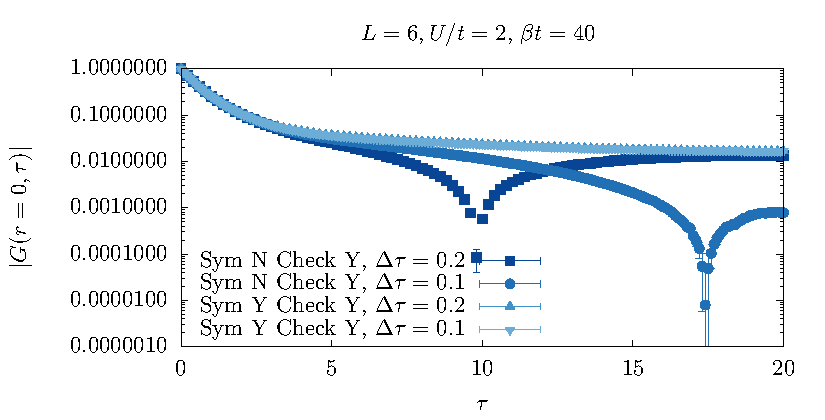
\includegraphics[width=0.49\textwidth]{Figures/Dtau_1/Dtau_1.pdf}
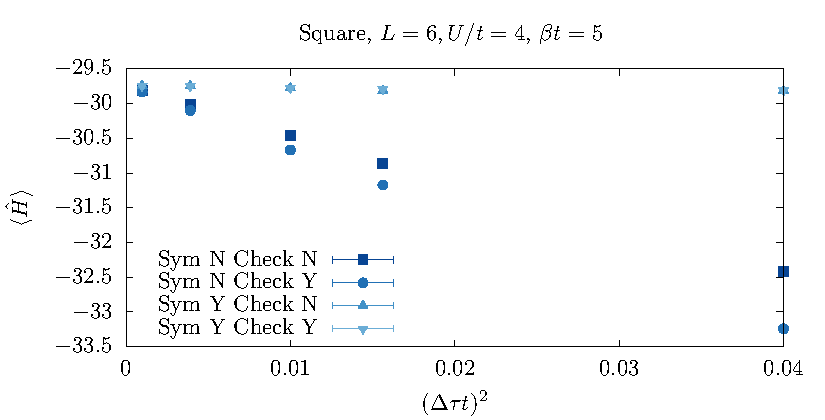
\includegraphics[width=0.49\textwidth]{Figures/Dtau/Dtau.pdf}

\caption{Analysis of  Trotter systematic error.   
        Left:    We consider a $6 \times 6$ Hubbard model on the Honeycomb lattice, $U/t=2$, half-band filling,  inverse temperature $\beta t =40$,  and we have used Hubbard-Stratonovich transformation that couples to  the density.    The figure plots the  local-time displaced Green function.
        Right: Here we consider the $6\times 6$ Hubbard model at $U/t=4$, half-band filling,  inverse temperature $\beta t =5$, and we have used the Hubbard Stratonovich transformation that couples to the z-component of spin.  We provide data for the four combinations of  the logical variables \texttt{Symm}  and \texttt{Checkerboard}, where  \texttt{Symm=.true.}  (\texttt{.false.})  indicates a symmetric  (asymmetric) Trotter decomposition has been used, and  \texttt{Checkerboard=.true.}  (\texttt{.false.})   that the  checkerboard   decomposition  for the hopping  matrix has (not) been used. 
  }
        \label{Trotter.fig}
\end{figure}


\subsubsection{ The \texttt{Symm} flag } 


If the  \texttt{Symm}   \index{\texttt{Symm}} flag is set to true,  then the program will automatically --  for the set of predefined lattices  and models -- use the symmetric   $\Delta \tau$ time step  of the interaction and 
hopping terms.   

To save CPU time  when the \texttt{Symm}  flag is on  we  carry out the following   approximation:
\begin{equation}
	\left[  
	  \left(\prod_{j=1}^{N_T-1} e^{-\frac{\Delta \tau}{4} \hat{T}_j } \right)    e^{-\frac{\Delta \tau}{2} \hat{T}_{N_T} }    
   \left(  \prod_{j=N_T-1}^{1} e^{-\frac{\Delta \tau}{4} \hat{T}_j } \right)      \right]^2   \simeq
	  \left(\prod_{j=1}^{N_T-1} e^{-\frac{\Delta \tau}{2} \hat{T}_j } \right)    e^{-\Delta \tau\hat{T}_{N_T} }    
   \left(  \prod_{j=N_T-1}^{1} e^{-\frac{\Delta \tau}{2} \hat{T}_j } \right).   
\end{equation}
The above  is consistent with the overall precision of the Trotter decomposition and more importantly  conserves the Hermiticity of the propagation. 

%-----------------------------------------------------------------------------------
\subsection{Stabilization - a peculiarity of the BSS algorithm}\label{sec:stable}
%-----------------------------------------------------------------------------------
%
From the partition function in Eq.~\eqref{eqn:partition_2} it can be seen that, for the calculation of the Monte Carlo weight and of the observables, a long product of matrix exponentials has to be formed.
In addition to that, we need to be able to extract the single-particle Green function  for a given flavor index at, say, time slice $\tau = 0$.  As  mentioned above (cf. Eq.~\eqref{eqn:Green_eq}), this quantity is given by: 
\begin{equation}
\bm{G}= \left( \mathds{1} + \prod_{ \tau= 1}^{L_{\text{Trotter}}} \bm{B}_\tau \right)^{-1},
\end{equation}
which can be recast as the more familiar linear algebra problem of finding a solution for the linear system
\begin{equation}
\left(\mathds{1} + \prod_\tau \bm{B}_\tau\right) x = b.
\end{equation}
The matrices $\bm{B}_\tau \in \mathbb{C}^{n\times n}$ depend on the lattice size as well as other physical parameters that can be chosen such that a matrix norm of $\bm{B}_\tau$ can be unbound in size.
From standard perturbation theory for linear systems, the computed solution $\tilde{x}$ would 
contain a relative error
\begin{equation}
\frac{|\tilde{x} - x|}{|x|} = \mathcal{O}\left(\epsilon \kappa_p\left(\mathds{1} + \prod_\tau \bm{B}_\tau\right)\right),
\end{equation}
where $\epsilon$ denotes the machine precision, which is $2^{-53}$ for IEEE double-precision numbers, and $\kappa_p(\bm{M})$ is the condition number of the matrix $\bm{M}$ with respect to the matrix $p$-norm. Due to $\prod_ \tau \bm{B}_\tau$ containing exponentially large and small scales, as can be seen in Eq.~\eqref{eqn:partition_2}, a straightforward inversion turns out to be completely ill-suited. That would lead the condition number, as a function of increasing inverse temperature, to grow exponentially, rendering the computed solution $\tilde{x}$ meaningless.

In order to circumvent this, more sophisticated methods have to be employed. As a first step, assuming that the multiplication of \texttt{NWrap} $\bm{B}$ matrices has an acceptable condition number and, for simplicity, that \texttt{NWrap} is a divisor of $L_{\text{Trotter}}$, we can write:
%\begin{equation}
%\bm{G} = \left( \mathds{1} + \prod\limits_{ i = 0}^{\frac{L_{\text{Trotter}}} {\texttt{NWrap} -1}}       \underbrace{\prod_{\tau=1}^{\texttt{NWrap}} \bm{B}_{i  \cdot  \texttt{NWrap}+ \tau} }_{ \equiv \mathcal{\bm{B}}_i}\right)^{-1}.
%\end{equation}
\begin{equation}
\bm{G} = \left( \mathds{1} + \prod\limits_{ i = 1}^{\frac{L_{\text{Trotter}}} {\texttt{NWrap}}}       \underbrace{\prod_{\tau=1}^{\texttt{NWrap}} \bm{B}_{(i-1)  \cdot  \texttt{NWrap}+ \tau} }_{ \equiv \mathcal{\bm{B}}_i}\right)^{-1}.
\end{equation}
The default stabilization strategy in the auxiliary-field QMC implementation of the ALF project, is then to form a product of QR-decompositions, which was proven to be weakly backwards stable in \cite{Bai2011}.
The key idea is to efficiently separate the scales of a matrix from the orthogonal part of a matrix.
This can be achieved using a QR decomposition of a matrix $\bm{A}$ in the form $\bm{A}_i = \bm{Q}_i \bm{R}_i$. The matrix $\bm{Q}_i$ is unitary and hence in the usual $2$-norm it holds that $\kappa_2(\bm{Q}_i) = 1$.
To get a handle on the condition number of $\bm{R}_i$ we will form the
diagonal matrix
\begin{equation}
(\bm{D}_i)_{n,n} = |(\bm{R}_i)_{n,n}|
\label{eq:diagnorm}
\end{equation}
and set $\tilde{\bm{R}}_i = \bm{D}_i^{-1} \bm{R}_i$
This gives the decomposition
\begin{equation}
\bm{A}_i = \bm{Q}_i \bm{D}_i \tilde{\bm{R}}_i.
\end{equation}
The matrix $\bm{D}_i$ now contains the row norms of the original $\bm{R}_i$ matrix and hence attempts to separate off the total scales of the problem from $\bm{R}_i$.
This is similar in spirit to the so-called matrix equilibration which tries to improve the condition number of a matrix through suitably chosen column and row scalings.
Due to a theorem by van der Sluis \cite{vanderSluis1969} we know that the choice in Eq.~\eqref{eq:diagnorm} is almost optimal among all diagonal matrices $\bm{D}$ from the space of diagonal matrices $\mathcal{D}$, in the sense that
\begin{equation*}
\kappa_p((\bm{D}_i)^{-1} \bm{R}_i ) \leq n^{1/p} \min_{\bm{D} \in \mathcal{D}} \kappa_p(\bm{D}^{-1} \bm{R}_i).
\end{equation*}
Now, given an initial decomposition of $\bm{A}_{j-1} = \prod_i \mathcal{\bm{B}}_i = \bm{Q}_{j-1} \bm{D}_{j-1} \bm{T}_{j-1}$ an update
$\mathcal{\bm{B}}_j \bm{A}_{j-1}$ is formed in the following three steps:
\begin{enumerate}
\item Form $ \bm{M}_j = (\mathcal{\bm{B}}_j \bm{Q}_{j-1}) \bm{D}_{j-1}$. Note the parentheses.
\item Do a QR decomposition of $\bm{M}_j = \bm{Q}_j \bm{D}_j \bm{R}_j$. This gives the final $\bm{Q}_j$ and $\bm{D}_j$.
\item Form the updated $\bm{T}$ matrices $\bm{T}_j = \bm{R}_j \bm{T}_{j-1}$.
\end{enumerate}
%While this provides provides a stable method to calculate the involved matrix product
%it can be pretty expensive. Therefore the user can specify to skip a certain number of 
%QR Decompositions and perform plain multiplications instead. This is specified in the parameters file by the \path{NWrap} parameter.
%\path{NWrap}~=~1 corresponds to always performing QR decompositions whereas larger integers give longer intervals where no QR decomposition will be performed.
The effectiveness of the stabilization \emph{has} to be judged for every simulation from the output file \path{info} (Sec.~\ref{sec:output_obs}). For most simulations there are two values to look out for:
\begin{itemize}
\item \texttt{Precision Green} \index{\texttt{Precision Green} }
\item \texttt{Precision Phase} \index{\texttt{Precision Phase}}
\end{itemize}
The Green function, as well as the average phase, are usually numbers with a magnitude of $\mathcal{O} (1)$. 
For that reason we recommend that \path{NWrap} \index{\path{NWrap}} is chosen such that the mean precision is of the order of $10^{-8}$ or better (or further recommendations see Sec.~\ref{sec:optimize}).
We include typical values of \texttt{Precision Phase} and of the mean and the maximal values of \texttt{Precision Green} in the example simulations discussed in Sec.~\ref{sec:prec_spin}.

% !TEX root = doc.tex
% Copyright (c) 2016 The ALF project.
% This is a part of the ALF project documentation.
% The ALF project documentation by the ALF contributors is licensed
% under a Creative Commons Attribution-ShareAlike 4.0 International License.
% For the licensing details of the documentation see license.CCBYSA.
%
%------------------------------------------------------------
\subsection{Monte Carlo sampling}\label{sec:sampling}
%------------------------------------------------------------
%
Error estimates  in Monte Carlo simulations  can be  delicate and are based on the central limit theorem \cite{Negele}. This theorem requires independent 
measurements and  a finite variance.
In this subsection we will give examples of the issues that a user will have to look out for while 
using a Monte Carlo code. Those effects are part of the common lore of the field
and we can only touch on them briefly  in this text.
For a deeper understanding of the inherent issues of Markov chain Monte Carlo methods 
we refer the reader to the pedagogical introduction in chapter 1.3.5 of Krauth\cite{Krauth2006}, the overview article of Sokal~\cite{Sokal89},  the more specialized literature by Geyer~\cite{Geyer1992} and chapter 6.3 of Neal~\cite{neal1993}. 

In general, one distinguishes local from global updates. As the name suggest, the local update corresponds to a small change of the configuration, e.g. a single spin flip of one of the $L_{\mathrm{Trotter}}(M_I+M_V)$ field entries (see Sec.~\ref{sec:updating}), whereas a global update changes a significant part of the configuration. The default update scheme of the implementation at hand are local updates such that a minimum amount of moves is required to generate a independent configuration. The associated time scale is called  the autocorrelation time, $T_\mathrm{auto}$, and is generically dependent upon the choice of the observables. 

 Our unit of \textit{sweeps} is defined such that each field is visited twice in a sequential propagation from $\tau = 0$ to $\tau = L_{\text{ Trotter}}$  and back.  A single sweep will  generically not  suffice to produce an independent  configuration.
In fact, the autocorrelation time $T_\mathrm{auto}$ characterizes the required time scale to generate an independent  values of $\langle\langle\hat{O}\rangle\rangle_C$ for the observable $O$. This has several consequences for the Monte Carlo simulation:
\begin{itemize}
	\item First of all, we start from a randomly chosen field configuration such that one has to invest \textit{at least}  one, but generically much more, $T_\mathrm{auto}$ to generate relevant, equilibrated configurations before reliable measurements are possible. This phase of the simulation is known as the warm-up or burn-in phase. In order to keep the code as flexible as possible (different simulations might have different autocorrelation times), measurements are taken from the very beginning. Instead, we provide the parameter \path{n_skip} for the analysis to ignore the first \path{n_skip} bins.
	\item Secondly, our implementation averages over a given amount of measurements   set by the variable \texttt{NSWEEPS}  before storing the results, known as one bin, on the disk.  A bin corresponds to \texttt{NSWEEPS}  sweeps. The  error analysis requires statistically  independent bins to generate reliable confidence estimates. If bins are to small (averaged over a period shorter then $T_\mathrm{auto}$), the error bars are then typically underestimated. Most of the time, the autocorrelation time is unknown before the simulation is started.  Sometimes the used compute cluster does not allow single runs long enough to generate appropriately sized bins. Therefore, we provide the \path{N_rebin} parameter that specifies how many bins are combined into a new bin during the error analysis. In general, one should check that a further increase of the bin size does not change the error estimate   (For an explicit example, the reader is referred to Sec.~\ref{sec:autocorr} and the appendix of Ref.~\cite{Assaad02}).

The \path{N_rebin} variable can be used to control a second issue. The distribution of the Monte Carlo estimates $\langle\langle\hat{O}\rangle\rangle_C$ is unknown. The result in the form $(\mathrm{mean}\pm \mathrm{error})$ assumes a Gaussian distribution. Every original distribution with a finite variance turns into a Gaussian one, once it is folded often enough (central limit theorem). Due to the internal averaging (folding) within one bin, many observables are already quite Gaussian. Otherwise one can increase \path{N_rebin} further, even if the bins are already independent~\cite{Bercx17}.
	\item The third issue concerns time displaced correlation functions. Even if the configurations are independent, the fields within the configuration are still correlated. Hence, the data for $S_{\alpha,\beta}(\vec{k},\tau)$ (see Sec.~\ref{sec:obs}; Eqn.~\ref{eqn:s}) and $S_{\alpha,\beta}(\vec{k},\tau+\Delta\tau)$ are also correlated. Setting the switch \path{N_Cov = 1} triggers the calculation of the covariance matrix in addition to the usual error analysis. The covariance is defined by
	\begin{equation}
		COV_{\tau \tau'}=\frac{1}{N_{\text{Bin}}}\left\langle\left(S_{\alpha,\beta}(\vec{k},\tau)-\langle S_{\alpha,\beta}(\vec{k},\tau)\rangle\right)\left(S_{\alpha,\beta}(\vec{k},\tau')-\langle S_{\alpha,\beta}(\vec{k},\tau')\rangle\right)\right\rangle\,.
	\end{equation}
An example where this information is necessary is the  calculation of mass gaps extracted by fitting the  tail  of the time displaced correlation function.  Omitting  the covariance matrix will  underestimate the  error.
\end{itemize}


%
%--------------------------------------------------------------
\subsubsection{The Jackknife resampling method}\label{sec:jack}
%--------------------------------------------------------------
%
For each observable $\hat{A}, \hat{B},\hat{C} \cdots$ the Monte Carlo program computes a data set of $N_{\text{Bin}}$ (ideally) independent values where for each observable the measurements belong to the same  statistical distribution.  In the general case, we would like to evaluate a function of expectation values, $f(\langle \hat{A} \rangle, \langle \hat{B} \rangle, \langle \hat{C} \rangle  \cdots)$ --
see for example the expression (\ref{eqn:obs_rw}) for the observable including reweighting --
and are interested in the statistical estimates of its mean value  and the standard error of the mean.
A numerical method for the statistical analysis of a given function $f$ which properly handles error propagation and correlations among the observables is the Jackknife method, which is, like the related Bootstrap method, a resampling scheme \cite{efron1981}.
Here we briefly review the \textit{delete-1 Jackknife} scheme which is based on the idea to generate $N_{\text{bin}}$ new data sets of size $N_{\text{bin}}-1$ by consecutively removing one data value from the original set. By $A_{(i)}$ we denote the arithmetic mean for the observable $\hat{A}$, without the $i$-th data value $A_{i}$, namely
\begin{equation}
A_{(i)} \equiv \frac{1}{N_{\text{Bin}}-1} \sum\limits_{k=1,\,k\neq i}^{N_{\text{Bin}}} A_{k}\;.
\end{equation}
As the corresponding quantity for  the function $f(\langle \hat{A} \rangle, \langle \hat{B} \rangle, \langle \hat{C} \rangle  \cdots)$, we define 
\begin{equation}
f_{(i)}(\langle \hat{A} \rangle, \langle \hat{B} \rangle, \langle \hat{C} \rangle  \cdots) \equiv
f( A_{(i)}, B_{(i)},C_{(i)}\cdots)\;.
\end{equation}
Following the convention in the literature, we will denote the final Jackknife estimate of the mean by $f_{(\cdot)}$ and its standard error by $\Delta f$. The Jackknife mean is  given by
\begin{equation}
\label{eqn:jack_mean}
f_{(\cdot)}(\langle \hat{A} \rangle, \langle \hat{B} \rangle, \langle \hat{C} \rangle  \cdots) =
\frac{1}{N_{\text{Bin}}}\sum\limits_{i=1}^{N_{\text{Bin}}} f_{(i)}(\langle \hat{A} \rangle, \langle \hat{B} \rangle, \langle \hat{C} \rangle  \cdots)\;,
\end{equation}
and the standard error, including bias correction, is given by
\begin{equation}
\label{eqn:jack_error}
(\Delta f)^{2} = 
\frac{N_{\text{Bin}}-1}{N_{\text{Bin}}} \sum\limits_{i=1}^{N_{\text{Bin}}}
\left[f_{(i)}(\langle \hat{A} \rangle, \langle \hat{B} \rangle, \langle \hat{C} \rangle  \cdots)
- f_{(\cdot)}(\langle \hat{A} \rangle, \langle \hat{B} \rangle, \langle \hat{C} \rangle  \cdots)\right]^{2}\;.
\end{equation}
In case of $f=\langle\hat A\rangle$, the results (\ref{eqn:jack_mean}) and (\ref{eqn:jack_error}) reduce to the plain sample average and the standard, bias corrected, estimate of the error.

%
%--------------------------------------------------------------------------
\subsubsection{An explicit example of error estimation}\label{sec:autocorr}
%---------------------------------------------------------------------------
%
In the following we use one of our examples, the Hubbard model on a square lattice in the $M_z$ Hubbard-Stratonovich decoupling (see Sec.~\ref{sec:walk1.1}), to show explicitly how to estimate errors.  We will equally show that the  autocorrelation time is dependent upon the  choice of the observable.  In fact, different observables within the same run can have different autocorrelation times  and of course, this time scale depends on the  parameter choice.  Hence, the user has to check  autocorrelations of individual observables for each simulation!  Typical regions of the phase diagram that require special attention are critical points  where length scales diverge.  

To determine the autocorrelation time, we calculate the correlation function
\begin{equation}
\label{eqn:autocorrel}
	Auto_{\hat{O}}(t_{\textrm{QMC}})=\sum_{i=0}^{N_{\textrm{Bin}}-t_{\textrm{QMC}}}\frac{\left(O_i-\left\langle \hat{O}\right\rangle \right)\left(O_{i+t_{\textrm{QMC}}}-\left\langle \hat{O}\right\rangle \right)}{\left(O_i-\left\langle \hat{O}\right\rangle \right)\left(O_{i}-\left\langle \hat{O}\right\rangle \right)}\, ,
\end{equation}
where $O_i$ refers to the Monte Carlo estimate of the observable $\hat{O}$ in the $i^{\text{th}}$ bin. This function typically shows an exponential decay and the decay rate defines the autocorrelation time.
%
\begin{figure}
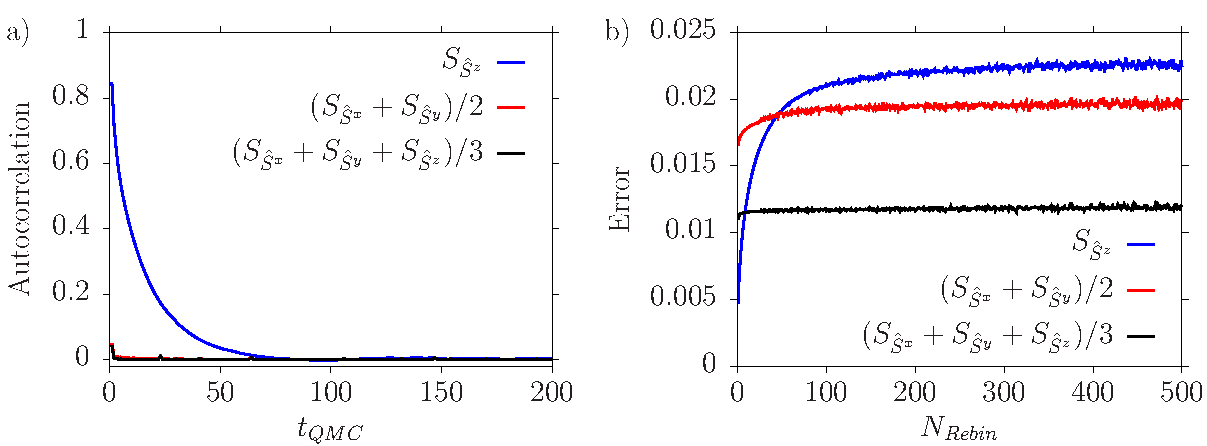
\includegraphics[width=1.0\textwidth]{Figures/fig1.pdf}
	\caption{\label{fig_autocorr}
	        The autocorrelation function $Auto_{\hat{O}}(t_{\textrm{QMC}})$ (a) and the scaling of the error with effective bin size (b) of three equal time spin-spin correlation functions $\hat{O}$ of the Hubbard model in the $M_z$ decoupling (see Sec.~\ref{sec:walk1.1}). Simulations were done on a $ 6 \times 6$ square lattice, with  $U/t=4$ and $\beta t = 6$.  The original bin contained only one sweep and we calculated around one million bins on a single core. The different  autocorrelation times for the $xy$-plane compared to the $z$-direction can be detected from the decay rate of the autocorrelation function (a) and from the point where saturation of the error sets in (b), which defines the required effective bin size for independent measurements. Apparently and as argued in the text, the  improved estimator $(S_{\hat{S}^{x}} + S_{\hat{S}^{y}}+ S_{\hat{S}^{z}})/3$  has the smallest autocorrelation time.
 }
\end{figure}
%
Figure~\ref{fig_autocorr} (a) shows the autocorrelation functions $Auto_{\hat{O}}(t_{\textrm{QMC}})$ for three spin-spin-correlation functions [Eq.~(\ref{eqn:s})] at momentum $\vec{k}=(\pi,\pi)$ and at $\tau=0$: 

$\hat{O} = S_{\hat{S}^{z}}$ for the $z$ spin direction, 
$\hat{O} =(S_{\hat{S}^{x}} + S_{\hat{S}^{y}})/2$ for the $xy$ plane, and
$\hat{O} =(S_{\hat{S}^{x}} + S_{\hat{S}^{y}}+ S_{\hat{S}^{z}})/3$ for the total spin.
 The Hubbard model  has a $SU(2)$ spin symmetry. However, we chose a HS field which couples to the $z$-component of the magnetization,  $M_z$,  such that each configuration breaks this symmetry. Of course, after Monte Carlo averaging one expects restoration of the symmetry. The model, on bipartite  lattices,  shows spontaneous spin-symmetry breaking at $T=0$ and in the thermodynamic limit.  At finite temperatures, and within the so-called renormalized classical regime,  quantum antiferromagnets have a length scale  that  diverges  exponentially  with decreasing temperatures \cite{Chakravarty88}.     
The parameter set chosen for Fig.~\ref{fig_autocorr}  is non-trivial in the sense that it places the Hubbard model in this renormalized classical regime where the correlation length is substantial.  Figure~\ref{fig_autocorr}  clearly shows a very short autocorrelation time for the $xy$-plane whereas we detect a considerably longer  autocorrelation time  for the $z$-direction.  This is a direct consequence of the {\it long} magnetic length scale and the chosen decoupling.
The physical reason for the long autocorrelation time  corresponds to  the restoration of the $SU(2)$ spin symmetry.    This insight can be used to define an improved, $SU(2)$ symmetric estimator for the spin-spin correlation function, namely
$(S_{\hat{S}^{x}} + S_{\hat{S}^{y}} + S_{\hat{S}^{z}})/3$. 
 Thereby, global spin rotations are no longer an issue and this improved estimator  shows the shortest autocorrelation time as seen clearly in Fig.~\ref{fig_autocorr} (b). Other ways to tackle large autocorrelation can be global updates or parallel tempering.

Using the time series of Monte Carlo samples we would like to obtain estimates of the mean and the standard error of the mean.
A simple method which we will describe in this tutorial is the rebinning method, also known in the literature as rebatching, where a fixed number (denoted by \path{N_rebin}) of adjacent original bins are aggregated to form a new effective bin.
In addition to measuring the decay rate of the autocorrelation function (\ref{eqn:autocorrel}), a measure for the autocorrelation time  can be also obtained by the rebinning method. 
For a comparison to other methods of estimating the autocorrelation time we refer the reader to the literature \cite{Thompson2010, Geyer1992, neal1993}.
A reliable error analysis requires independent bins, otherwise the error is typically underestimated. This behavior is observed in Fig.~\ref{fig_autocorr} (b), where the effective bin size has been systematically increased by rebinning. If the effective bin size is smaller than the autocorrelation time the error will be underestimated. When the effective bin size becomes  larger than the autocorrelation time converging behavior sets in and in this region the error estimate will be correct.

For the analysis of the Monte Carlo data (see Sec.~\ref{sec:analysis}), the user can provide a finite value for \path{N_auto} to trigger the computation of  autocorrelation functions $Auto_{\hat{O}}(t_{\textrm{QMC}})$ in the range $t_{\text{QMC}}=[0,\textrm{\path{N_auto}}]$. 
Since these computations are quite time consuming and require many Monte Carlo bins the default value is  \path{N_auto=0} if unspecified. To produce Fig.~\ref{fig_autocorr}, we set $\textrm{\path{N_auto}}=500$ and used a total of approximately one million bins.


% !TEX root = doc.tex
% Copyright (c) 2017 The ALF project.
% This is a part of the ALF project documentation.
% The ALF project documentation by the ALF contributors is licensed
% under a Creative Commons Attribution-ShareAlike 4.0 International License.
% For the licensing details of the documentation see license.CCBYSA.
%
%------------------------------------------------------------
\subsection{Pseudocode description}\label{sec:pseudocode}
%------------------------------------------------------------
%

The Monte Carlo algorithm as implemented in ALF can be summarized as follows:

\begin{mdframed}[frametitle={Basic structure of the auxiliary-field QMC implementation (\path{Prog/main.F90}):}]
{\setlength{\parindent}{0pt}
Set the Hamiltonian and the lattice:\\
\textbf{Call} ham\_set\\
Read in an auxiliary-field configuration or generate it randomly:\\
\textbf{Call} field\%in\\

This loop fills the storage needed for the first actual Monte Carlo sweep:\\
\textbf{Do} \texttt{ntau} from  \texttt{ltrot} to \texttt{1}\\
\hspace*{1em} Compute propagation matrices and store them at the stabilization points:\\
\hspace*{1em} \textbf{Call} wrapul\\
\textbf{Enddo}\\
 
Loop over bins: \\
\textbf{Do} \texttt{nbc} from  \texttt{1} to \texttt{nbin} \\
\hspace*{1em} Loop over sweeps. Each sweep updates twice (upward and downward in time) the whole\\
\hspace*{1em} space-time lattice of auxiliary fields. The sweep defines the unit of Monte Carlo time:\\
%\hspace*{1em} The sweep defines the unit of Monte Carlo time:\\
\hspace*{1em} \textbf{Do} \texttt{nsw} from  \texttt{1} to \texttt{nsweep}  \\
\hspace*{2em} Upward sweep:\\
\hspace*{2em} \textbf{Do} \texttt{ntau} from \texttt{1} to \texttt{ltrot}\\      
\hspace*{3em} Propagate the Green function from time \texttt{ntau$-$1} to \texttt{ntau}, and compute a new\\
\hspace*{3em} estimate (using sequential update scheme) of the Green function at \texttt{ntau}: \\
\hspace*{3em} \textbf{Call} wrapgrup\\
         
\hspace*{3em}  Stabilization: \\     
\hspace*{3em} \textbf{If} \texttt{ntau} equals stabilization point in imaginary time \textbf{then}\\
\hspace*{4em} Compute propagation matrix from previous stabilization point to \texttt{ntau}: \\
\hspace*{4em} \textbf{Call} wrapur\\
\hspace*{4em} Read from storage: propagation from \texttt{ltrot} to \texttt{ntau}\\
\hspace*{4em} Write to storage: the just-computed propagation \\
\hspace*{4em} Recalculate the Green function at time \texttt{ntau} in a stable way:\\
\hspace*{4em} \textbf{Call} cgr\\            
\hspace*{4em} Check the precision between propagated and recalculated Green functions:\\
\hspace*{4em} \textbf{Call} control\_precisionG\\
\hspace*{3em} \textbf{Endif}\\
    
\hspace*{3em} Measure the equal-time observables: \\
\hspace*{3em} \textbf{If} \texttt{ntau} is in the intervall \texttt{[LOBS\_ST, LOBS\_EN]} \textbf{then}\\
\hspace*{4em} \textbf{Call} obser\\
\hspace*{3em} \textbf{Endif}\\
\hspace*{2em} \textbf{Enddo}\\

\hspace*{2em} Downward sweep:\\
\hspace*{2em} \textbf{Do} \texttt{ntau} from \texttt{ltrot} to \texttt{1}\\
\hspace*{3em} Repeat the above steps (update, propagation, stabilization, equal-time measurements) \\
\hspace*{3em} for the downward direction in imaginary time\\
\hspace*{2em} \textbf{Enddo}\\

\hspace*{2em} Measure the time-displaced observables: \\
\hspace*{2em} \textbf{Call} tau\_m\\
\hspace*{1em} \textbf{Enddo} (loop over sweeps)\\
    
\hspace*{1em} Calculate measurement averages for current bin and write them to disk:\\
\hspace*{1em} \textbf{Call} pr\_obs\\
\hspace*{1em} Write auxiliary-field configuration to disk: \\
\hspace*{1em} \textbf{Call} field\%out\\
\textbf{Enddo} (loop over bins)\\
% 
% Write the \texttt{info} file to disk:\\
% \textbf{call} control\_print
}
\end{mdframed}
% 
% 
% \lstset{style=fortran_pseudo_code}
% \begin{lstlisting}
% 
% ! Set the Hamiltonian and the lattice:
% call ham_set
% 
% ! Read in an auxiliary-field configuration or generate it randomly:
% call confin
% 
% ! This loop fills the storage, needed for the first actual Monte Carlo sweep:
% do ntau = ltrot, 1, -1 
%    ! Compute propagation matrices and store them at the stabilization points:
%    call wrapul 
% enddo
% 
% ! Loop over bins. The bin defines the unit of Monte Carlo time:
% do nbc = 1, nbin 
% 
%    ! Loop over sweeps. Each sweep updates twice (sweeping upward and downward in time)
%    ! the whole space-time lattice of auxiliary fields:
%    do nsw = 1, nsweep 
%    
%       ! Upward sweep:
%       do ntau = 1, ltrot
%       
%          ! Propagate the Green function from time ntau -1 to ntau, 
%          ! and compute new estimate (using sequential update scheme) of Green at ntau: 
%          call wrapgrup
%          
%          ! Stabilization:      
%          if (ntau == stabilization point)
%             ! Compute propagation matrix from previous stabilization point to ntau: 
%             call wrapur
%             ! Read from storage: propagation from ltrot to ntau
%             ! Write to storage : the just computed propagation 
%                         
%             ! Recalculate Green function at time ntau in a stable way:
%             call cgr
%             
%             ! Check the precision between propagated and recalculated Green function
%          endif
%         
%          ! Measure the equal time observables, 
%          ! if ntau is in the measuring range [LOBS_ST, LOBS_EN]:
%          call obser
%       enddo
%       
%       ! Downward sweep:
%       do ntau = ltrot, 1, -1
%          ! Repeat the above steps (update, propagation, stabilization, measurements) 
%          ! for the downward direction in imaginary time
%       enddo
%       
%    enddo ! Loop over sweeps
%     
%    ! Calculate averages of the measurements of the previous bin and write to disk
%    ! Write auxiliary-field configuration to disk
%    
% enddo ! Loop over bins        
% 
% \end{lstlisting}

\section{Data Structures and Input/Output}\label{sec:imp}
% Copyright (c) 2016 The ALF project.
% This is a part of the ALF project documentation.
% The ALF project documentation by the ALF contributors is licensed
% under a Creative Commons Attribution-ShareAlike 4.0 International License.
% For the licensing details of the documentation see license.CCBYSA.

% !TEX root = Doc.tex
%------------------------------------------------------------
\subsection{Implementation of the Hamiltonian \& the lattice} 
%------------------------------------------------------------

In general, the module \path{Hamiltonian} defines the model Hamiltonian, the lattice under consideration and the desired observables (Table~\ref{table:hamiltonian}). 
We have collected a number of example Hamiltonians, lattices and observables in the file  \path{Hamiltonian_Examples.f90}.  They are described in the Sec.~\ref{sec:walk1} - \ref{sec:walk2}.
To implement a user-defined model, only the module \path{Hamiltonian} has to be set up. Accordingly, this documentation focusses almost entirely  on this module and the subprograms it includes. 
The remaining parts of the code may be treated as as a black box.  

To specify the Hamiltonian, one needs  an  \path{Operator} and \path{Lattice} type as well as a type for the observables. These three data structures will be described in the following. 

%
\begin{table}[h]
    \begin{tabular}{@{} l l l @{}}\toprule
    Subprogram & Description & Section \\\midrule
    \hl{\texttt{Ham\_Set}}  & Reads in model and lattice parameters from the file \texttt{parameters}. \\
                       & And it sets the Hamiltonian by calling \texttt{Ham\_latt}, \texttt{Ham\_hop}, and \texttt{Ham\_V}. & \\
    \hl{\texttt{Ham\_hop}}  & Sets the hopping term  $\hat{\mathcal{H}}_{T}$ by calling \texttt{Op\_make} and \texttt{Op\_set}. & \ref{sec:op}, \ref{sec:specific}\\
    \hl{\texttt{Ham\_V}}    & Sets the interaction terms  $\hat{\mathcal{H}}_{V}$ and $\hat{\mathcal{H}}_{I}$ 
                         by calling \texttt{Op\_make} and \texttt{Op\_set}.& \ref{sec:op}, \ref{sec:specific}\\  
    \hl{\texttt{Ham\_Latt}} & Sets the lattice by calling \texttt{Make\_Lattice}.& \ref{sec:latt}\\
    \hl{\texttt{S0}}        & A function which returns an update ratio for the Ising term $\hat{\mathcal{H}}_{I,0}$. 
    & \ref{sec:s0} \\
    \hl{\texttt{Alloc\_obs}} & Asigns memory storage to the observables & \\
    \hl{\texttt{Obser}}      & Computes the scalar observables and equal-time correlation functions. & \ref{sec:obs} \\
    \hl{\texttt{ObserT}}     & Computes time-displaced correlation functions. & \ref{sec:obs}\\
    \texttt{Init\_obs}  & Initializes the observables to zero. & \\    
    \texttt{Pr\_obs}    & Writes the observables to the disk by calling \texttt{Print\_bin}. \\\bottomrule    
   \end{tabular}
   \caption{Overview of the subprograms of the  module \texttt{Hamiltonian} to define the Hamiltonian, the lattice and the observables. 
   The highlighted subroutines have to be modified by the user.
    \label{table:hamiltonian}}
\end{table}
%

%------------------------------------------------------------
\subsubsection{The \texttt{Operator} type}\label{sec:op}
%------------------------------------------------------------

The fundamental data structure in the code is the derived data type \path{Operator}. 
This type is used to define the Hamiltonian (\ref{eqn:general_ham}).
In general, the matrices $\textbf{T}^{(ks)}$, $\text{V}^{(ks)}$ and $\textbf{I}^{(ks)}$ are sparse Hermitian matrices.
Consider the  matrix   ${\bm X}$ of dimension  $N_{\mathrm{dim}} \times N_{\mathrm{dim}}$, as an representative of each of the above three matrices.  Let us  denote  with  $ \left\{z_{1},\cdots,  z_{N}  \right\}$  a subset  of $N$ indices,  
for which
\begin{equation}
X_{x,y}  =
\left\{\begin{matrix}  X_{x,y}  &  \text{ if }   x,  y  \in \left\{ z_1, \cdots z_N \right\}\\ 
                                  0         &  \text{ otherwise } 
      \end{matrix}\right.
\end{equation}
 We define the $N \times N_{\mathrm{dim}}$ matrices $\mathbf{P}$  as
\begin{equation}
P_{i,x}=\delta_{z_{i},x}\;,
\end{equation}
where $i \in [1,\cdots, N ]$ and $ x  \in [1,\cdots, N_{\mathrm{dim}}]$. The matrix  $\bm{P}$ picks out the non-vanishing entries of $\bm{X}$, 
which are contained in the rank-$N$  matrix $\bm{O}$.  Thereby: 
\begin{equation}\label{eqn:xeqpdop}
\bm{X} =\bm{P}^{T} \bm{O} \bm{P}\;,
\end{equation}
such that:
\begin{equation}
X_{x,y} = \sum\limits_{i,j}^{N}  P_{i,x}  O_{i,j} P_{j,y}=\sum\limits_{i,j}^{N} \delta_{z_{i},x}  O_{ij} \delta_{z_{j},y} \;.
\end{equation}
Since  the  $\bm{P}$ matrices have only one non-vanishing entry per column,  they can be stored as a vector $\vec{P}$:
\begin{equation}
     P_i = z_i.
\end{equation}  
There are  many useful  identities which emerge from this  structure. For example: 
\begin{equation}
	e^{\bm{X}} =  e^{\bm{P}^{T} \bm{O} \bm{P}}   = \sum_{n=0}^{\infty}  \frac{\left( \bm{P}^{T} \bm{O} \bm{P} \right)^n}{n!} = \mathds{1}+ \bm{P}^{T} \left(e^{ \bm{O} }-\mathds{1} \right) \bm{P}
\end{equation}
since 
\begin{equation} 
	 \bm{P} \bm{P}^{T}= \mathds{1}_{N\times N}.
\end{equation}

In the code, we define a structure called \path{Operator} to capture the above. 
This type \path{Operator} bundles several components that are needed to define and use an operator matrix in the program.  

%------------------------------------------------------------
\subsubsection{Specification of the model}\label{sec:specific}
%------------------------------------------------------------
%
\begin{table}[h]
    \begin{tabular}{@{} l l l @{}}\toprule
    Variable & Type & Description \\\midrule
    \hl{\texttt{Op\_X\%N}}       & Integer     &  effective dimension $N$ \\
    \hl{\texttt{Op\_X\%O}}       & Complex    &  matrix  $\mathbf{O}$  of dimension $N \times N$\\
    \hl{\texttt{Op\_X\%P}}       & Integer   &  projection matrix $\mathbf{P}$  encoded as a vector of dimension $N$.\\
    \hl{\texttt{Op\_X\%g}}       & Complex    &  coupling strength $g$ \\  
    \hl{\texttt{Op\_X\%alpha}}   & Complex  &  constant $\alpha$ \\
    \hl{\texttt{Op\_X\%type}}    & Integer   &  parameter to set the type of 
                                             HS transformation\\
                             &   &  (1 = Ising, 2 = Discrete HS, for perfect square)  \\ 
    \texttt{Op\_X\%U}            & Complex &  matrix containing the eigenvectors of $\mathbf{O}$  \\
    \texttt{Op\_X\%E}            & Real &  eigenvalues of $\mathbf{O}$ \\
    \texttt{Op\_X\%N\_non\_zero} & Integer &  number of non-vanishing eigenvalues of $\mathbf{O}$ \\\bottomrule
   \end{tabular}
   \caption{Member Variables of the \texttt{Operator}  type. 
   In the left column, the letter \texttt{X} is a placeholder for the letters \texttt{T} and \texttt{V}, 
   indicating hopping and interaction operators, respectively.
   The highlighted variables have to be specified by the user.
  %  One will have to specify $N$, $O$, $P$, $g$, $\alpha$ and the type.  The other variables will be automatically generated in the routine \texttt{Op\_Set}.  
    \label{table:operator}}
\end{table}
%
In this section we show how to specify the  Hamiltonian (\ref{eqn:general_ham}) in the code. 
More precisely, we specify the Hamiltonian by setting  the matrices 
$ e^{-\Delta \tau {\bm T}^{(ks)}}$, $e^{  \sqrt{ \Delta \tau  U_k} \eta_{k\tau} {\bm V}^{(ks)} }$, and $e^{  -\Delta \tau s_{k\tau}  {\bm I}^{(ks)}}$ that appear in the 
partition function (\ref{eqn:partition_2}). 
To do so, we consider the general expression
\begin{equation}\label{eqn:exponent_mat}
e^{g \,\phi_{k\tau}(\texttt{type})\,\left(\mathbf{X} + \alpha\right)}\;,
\end{equation}
and store the following quantities in a variable of type \path{Operator} (see Table \ref{table:operator}):
the matrix $\mathbf{X}$ [see Eq.~(\ref{eqn:xeqpdop})], the constants $g$ and $\alpha$, and, optionally, also 
the type of the fields $\phi_{k\tau}(\text{type})$.  Either the fields
stem from the Ising term (\path{type=1}: $\phi_{k\tau}=s_{k\tau}$), or they result from the discrete Hubbard-Stratonovich transformation (\texttt{type=2}: $\phi_{k\tau}=\eta_{k\tau}$)).
 In general, we need  several arrays of variables of type \path{Operator}.
Since the implementation exploits the $SU(N_{\mathrm{col}})$ invariance of the Hamiltonian, we have dropped the color index $\sigma$ in the following.
\begin{itemize}
\item For the hopping Hamiltonian (\ref{eqn:general_ham_t}), we have to set the exponentiated hopping matrices $ e^{-\Delta \tau {\bm T}^{(ks)}}$: 

In this case $\mathbf{X}^{(ks)}=\mathbf{T}^{(ks)}$. Precisely, a single variable  \texttt{Op\_T}  describes the operator matrix
\begin{equation}
            \left( \sum_{x,y}^{N_{\mathrm{dim}}} \hat{c}^{\dagger}_x T_{xy}^{(ks)} \hat{c}^{\phantom{\dagger}}_{y}  \right)  \;,
\end{equation} 
where $k=[1, M_{T}]$ and $s=[1, N_{\mathrm{fl}}]$.  
To make contact with the general expression (\ref{eqn:exponent_mat}) we set $g=-\Delta \tau$, $\alpha = 0$. 
In case of the hopping matrix, the type variable $\texttt{Op\_T\%type}$  is neglected by the code. 
All in all, the corresponding array of structure variables is  \texttt{Op\_T(M$_T$,N$_{fl}$)}.

\item For the interaction Hamiltonian (\ref{eqn:general_ham_v}), which is of perfect-square type, we have to set the exponentiated matrices $e^{  \sqrt{ -  \Delta \tau  U_k} \eta_{k\tau} {\bm V}^{(ks)} }$:

In this case, ${\mathbf X}  = \mathbf{V}^{(ks)}$. A single variable  \texttt{Op\_V}  describes the operator matrix:
\begin{equation}
             \left[ \left( \sum_{x,y}^{N_{\mathrm{dim}}} \hat{c}^{\dagger}_x V_{x,y}^{(ks)} \hat{c}^{\phantom{\dagger}}_{y}  \right)  + \alpha_{ks} \right]  \;,
\end{equation} 
where $k=[1, M_{V}]$ and $s=[1, N_{\mathrm{fl}}]$. 
To make contact with the general expression (\ref{eqn:exponent_mat}), we set  $\alpha = \alpha_{ks}$ and $g = \sqrt{-\Delta \tau  U_k}$. 
The discrete Hubbard-Stratonovich decomposition which is used for the perfect-square interaction, is selected by setting the type variable to $\texttt{Op\_V\%type}=2$.
All in all, the required structure variables \texttt{Op\_V} are defined  using the array \texttt{Op\_V(M$_V$,N$_{fl}$)}.


\item For the Ising interaction Hamiltonian (\ref{eqn:general_ham_i}), we have to set the exponentiated matrices $e^{  -\Delta \tau s_{k\tau}  {\bm I}^{(ks)}}$:

In this case, $\bm{X}  = \bm{I}^{(k,s)} $.  
A single variable  \texttt{Op\_V} then  describes the operator matrix:
\begin{equation}
            \left( \sum_{x,y}^{N_{\mathrm{dim}}} \hat{c}^{\dagger}_x I_{xy}^{(ks)} \hat{c}^{\phantom{\dagger}}_{y}  \right)  \;,
\end{equation} 
where $k=[1, M_{I}]$ and $s=[1, N_{\mathrm{fl}}]$. 
To make contact with the general expression (\ref{eqn:exponent_mat}), we set $\alpha = 0$ and $g = -\Delta \tau$.
The Ising interaction is specified by setting the type variable  $\texttt{Op\_V\%type=1}$. 
All in all, the required structure variables are contained in the array \texttt{Op\_V(M$_{I}$,N$_{fl}$)}.

\item In case of a full interaction [perfect-square term (\ref{eqn:general_ham_v}) and Ising term (\ref{eqn:general_ham_i})],
we  define  the corresponding doubled array \texttt{Op\_V(M$_V$+M$_I$,N$_{fl}$) } and set the variables separately for both ranges of the array according to the above.  

\end{itemize}

%------------------------------------------------------------
\subsubsection{The \texttt{Lattice} type}\label{sec:latt}
%------------------------------------------------------------

We have a lattice module  which can generate one and two dimensional Bravais lattices.
Note that the orbital structure of each unit cell, has to be specified by the user in the Hamiltonian module. 
 The user has to specify unit vectors $\vec{a}_1$ and $\vec{a}_2$ as well as the size of the  lattice. The size is  characterized by  two vectors $\vec{L}_1$ and $\vec{L}_2$   and  the lattice is placed on a torus: 
\begin{equation}
	\hat{c}_{\vec{i} + \vec{L}_1 }  = \hat{c}_{\vec{i} + \vec{L}_2 }  = \hat{c}_{\vec{i}}
\end{equation}
The function call 
\begin{lstlisting} 
Call Make_Lattice( L1, L2, a1,  a2, Latt )
\end{lstlisting}
will generate the lattice   \texttt{Latt} of type \texttt{Lattice}.   Note that  the structure of the unit cell has to be provided by the user.    The reciprocal lattice vectors are defined by: 
\begin{equation}
\label{Latt.G.eq}
	\vec{a}_i  \cdot \vec{g}_i = 2 \pi \delta_{i,j}, 
\end{equation}
and the Brillouin zone corresponds to the Wigner Seitz cell of the lattice. 
With $\vec{k} = \sum_{i} \alpha_i  \vec{g}_i $, the  k-space quantization follows from: 
\begin{equation}
\begin{bmatrix}
	\vec{L}_1 \cdot \vec{g}_1  &  \vec{L}_1 \cdot \vec{g}_2  \\
	\vec{L}_2  \cdot \vec{g_1} & \vec{L}_2 \cdot  \vec{g}_2  
\end{bmatrix}
\begin{bmatrix}
   \alpha_1 \\
   \alpha_2
\end{bmatrix}
=
2 \pi 
\begin{bmatrix}
   n \\
   m
\end{bmatrix}
\end{equation}
such that 
\begin{eqnarray}
\label{k.quant.eq}
     \vec{k} =  n \vec{b}_1  + m \vec{b}_2 \text{  with  }   & &   \vec{b}_1 = \frac{2 \pi}{ (\vec{L}_1 \cdot \vec{g}_1)  (\vec{L}_2 \cdot  \vec{g}_2 )  - (\vec{L}_1 \cdot \vec{g}_2) (\vec{L}_2  \cdot \vec{g_1} ) }   \left[  (\vec{L}_2 \cdot  \vec{g}_2) \vec{g}_1 -   (\vec{L}_2  \cdot \vec{g_1} ) \vec{g}_2 \right] \text{   and  } \nonumber \\ 
        & & \vec{b}_2 = \frac{2 \pi}{ (\vec{L}_1 \cdot \vec{g}_1)  (\vec{L}_2 \cdot  \vec{g}_2 )  - (\vec{L}_1 \cdot \vec{g}_2) (\vec{L}_2  \cdot \vec{g_1} ) }   
           \left[  (\vec{L}_1 \cdot  \vec{g}_1) \vec{g}_2 -   (\vec{L}_1  \cdot \vec{g_2} ) \vec{g}_1 \right] 
\end{eqnarray}

%
\begin{table}[h]
   \begin{tabular}{@{} l l l @{}}\toprule
    Variable  & Type & Description \\\midrule
     \hl{\texttt{Latt\%a1\_p}, \texttt{Latt\%a2\_p}}   & Real     & Unit vectors $\vec{a}_1$,  $\vec{a}_2$ \\ 
     \hl{\texttt{Latt\%L1\_p}, \texttt{Latt\%L2\_p}}   & Real     & Vectors $\vec{L}_1$, $\vec{L}_2$ that define the topology of the  lattice. \\
     									  &              &  Tilted lattices are  thereby possible to implement.  \\
    \texttt{Latt\%N}                                                 &   Integer &  Number of lattice points, $N_{\text{unit cell}}$   \\
    \texttt{Latt\%list}                                               & Integer &  maps each lattice point $i=1,\cdots, N_{\text{unit cell}}$ to a real space vector\\ 
                                                                             &   &  denoting the position of the unit cell: \\
                                                                             &   & $\vec{R}_i$ = \texttt{list(i,1)} $\vec{a}_1$ +  \texttt{list(i,2)} $\vec{a}_2$  $  \equiv i_1  \vec{a}_1 + i_2  \vec{a}_2 $ \\
    \texttt{Latt\%invlist}                                        &  Integer &   \texttt{Invlist}$(i_1,i_2) = i $ \\
    \texttt{Latt\%nnlist}                                         &  Integer &   $j = \texttt{nnlist} (i, n_1, n_2) $,  $n_1, n_2 \in [-1,1] $ \\
                                                                           &              &    $\vec{R}_j = \vec{R}_i + n_1 \vec{a}_1  + n_2 \vec{a}_2 $ \\
   \texttt{Latt\%imj}                                             &   Integer  &  $ \vec{R}_{imj(i,j)}  =  \vec{R}_i -  \vec{R}_j$.        $imj, i, j \in  1,\cdots, N_{\text{unit cell}}$\\
    \texttt{Latt\%BZ1\_p}, \texttt{Latt\%BZ2\_p}  &   Real     & Reciprocal space vectors $\vec{g}_i$   (See Eq.~\ref{Latt.G.eq})\\
    \texttt{Latt\%b1\_p}, \texttt{Latt\%b1\_p}       &   Real     &  k-quantization (See Eq.~\ref{k.quant.eq}) \\
    \texttt{Latt\%listk}                                           &  Integer &  maps each reciprocal lattice point $k=1,\cdots, N_{\text{unit cell}}$\\
                                                                          &    & to a reciprocal space vector\\
                                                                          &     & $\vec{k}_k= \texttt{listk(k,1)} \vec{b}_1 +  \texttt{listk(k,2)} \vec{b}_2  \equiv k_1  \vec{b}_1 +   k_2  \vec{b}_2 $\\
    \texttt{Latt\%invlistk}                                     &    Integer    &   \texttt{Invlistk}$(k_1,k_2) = k $ \\
   \texttt{Latt\%b1\_perp\_p},  \\ 
   \texttt{Latt\%b2\_perp\_p}                             &    Real         &  Orthonormal vectors to $\vec{b}_i$.  For internal use. \\\bottomrule
   \end{tabular}
   \caption{Components of the \texttt{Lattice} type for two-dimensional lattices using as example the default lattice name \texttt{Latt}.
   The highlighted variables have to be specified by the user.  Other components of the Lattice will be generated  when calling: \texttt{ Call Make\_Lattice( L1, L2, a1,  a2, Latt )}. 
    \label{table:lattice}}
\end{table}
%

The \path{Lattice}  module equally handles  the Fourier transformation.  For example  the  subroutine  \path{Fourier_R_to_K}   carries out the  transformation: 
\begin{equation}
	S(\vec{k}, :,:,:) =  \frac{1}{N_{unit \,cell}}  \sum_{\vec{i},\vec{j}}   e^{-i \vec{k} \cdot \left( \vec{i}-\vec{j} \right)} S(\vec{i}  - \vec{j}, :,:,:)
\end{equation}
and  \path{Fourier_K_to_R}  the  inverse Fourier transform 
 \begin{equation}
	S(\vec{r}, :,:,:) =  \frac{1}{N_{unit \,cell}}  \sum_{\vec{k} \in BZ }   e^{ i \vec{k} \cdot \vec{r}} S(\vec{k}, :,:,:).
\end{equation}
In the above,   the unspecified dimensions of   structure factor can refer  to imaginary time,  and orbital indices. 

%--------------------------------------------------------------------------------------------
\subsection{The observable types \texttt{Obser\_Vec} and \texttt{Obser\_Latt}}\label{sec:obs}
%--------------------------------------------------------------------------------------------

Our definition  of the model includes observables [Eq.~(\ref{eqn:obs_rw})]. We have defined two observable types: \texttt{Obser\_vec}  for a array of scalar observables
such as the energy and  \texttt{Obser\_Latt}   for correlation functions that have the lattice symmetry. In the latter case, translation symmetry can be used to provide improved estimators and to reduce the size of the I/O.   
We also obtain improved estimators by taking measurements in the imaginary-time interval \texttt{[LOBS\_ST,LOBS\_EN]}  (see the parameter file in Sec.~\ref{sec:input}) thereby exploiting the invariance under translation in imaginary time.
Note that the translation symmetries  in space and in time are broken for a given  configuration $C$ but restored by the Monte Carlo sampling. 
In general, the user will define bins, each bins having a given amount of sweeps. Within a sweep we run sequentially trough the HS and Ising fields from   time slice 1 to $L_{\text{Trotter}}$ and back.  The results of each bin is written  in a file  and analyzed at the end of the run.     

To accomplish the reweighting of observables (see Sec.~\ref{sec:reweight}), for each configuration the measurement of an observable has to be multiplied by the factors \texttt{ZS} and \texttt{ZP}:
\begin{eqnarray}
\texttt{ZS} &=& \text{sign}(C)\;\\
\texttt{ZP} &=& \frac{e^{-S(C)}} {\Re \left[e^{-S(C)} \right]}\;,
\end{eqnarray}
They are computed from the Monte Carlo phase of a configuration,
\begin{equation}\label{eqn:phase}
	\texttt{phase}   =   \frac{e^{-S(C)}}{ \left| e^{-S(C) }\right| }\;,
\end{equation}
which is provided by the main program.


Note that each observable structure also includes the average sign [Eq.~(\ref{eqn:sign_rw})].

%---------------------------------
\subsubsection{Scalar observables}
%---------------------------------

This data type  is described in Table  \ref{table:Obser_vec} and  is useful to compute an array of  scalar observables.   Consider  a variable \texttt{Obs} of type  \texttt{Obser\_vec}.  At the beginning of each bin,  a call to  \texttt{Obser\_Vec\_Init} in the module \texttt{observables\_mod.f90}  will  set   \texttt{Obs\%N=0},   \texttt{Obs\%Ave\_sign =0}  and  \texttt{Obs\%Obs\_vec(:)=0}.  Each time the main  program calls the routine \texttt{Obser}  in the  \texttt{Hamiltonian} module,  the counter \texttt{Obs\%N}   is incremented by unity,   the sign  (see Eq.~\ref{Sign.eq}) is cumulated in the  variable \texttt{Obs\%Ave\_sign},  and the desired  the observables (multiplied by the sign and   $\frac{e^{-S(C)}} {\Re \left[e^{-S(C)} \right]}$, see Sec.~\ref{Observables.General})  are cumulated in the vector \texttt{Obs\%Obs\_vec}.  
%
\begin{table}[h]
   \begin{tabular}{@{} l l l l @{}}\toprule
    Variable  &  Type      &  Description &  Contribution of  \\
        &  & & configuration $C$ \\\midrule
    \texttt{Obs\%N}                       &  Int.        &   Number of measurements &\\
    \texttt{Obs\%Ave\_sign}               &  Real     &    Cumulated sign [Eq.~(\ref{eqn:sign_rw})] & $\text{sign}(C)$  \\
    \texttt{Obs\%Obs\_vec(:)}        & Compl.      &    Cumulated vector of observables [Eq.~(\ref{eqn:obs_rw})] &
           $ \langle \langle \hat{O}(:) \rangle \rangle_{C}\frac{e^{-S(C)}} {\Re \left[e^{-S(C)} \right]} \text{ sign }(C) $ \\
     \texttt{Obs\%File\_Vec}           &  Char.    &    Name of output file  &\\\bottomrule
   \end{tabular}
   \caption{Components of the \texttt{Obser\_vec}  type.  The table lists the data included in a variable  \texttt{Obs}  of type \texttt{Obser\_vec}.  
   % \mycomment{MB $\texttt{Obs\%Phase}$ is not $phase(C)$ but $sign(C)$. And the type of sign could in principle be reduced to integer.   }
         \label{table:Obser_vec}}
\end{table}
%
At the end of the bin, a call to  \texttt{Print\_bin\_Vec}   in  module \texttt{observables\_mod.f90}  will  append the result of the bin in the file  \texttt{File\_Vec}\_scal.  Note that this subroutine will automatically append the suffix  \_scal 
to the the filename \texttt{File\_Vec}.    This suffix  is important to allow automatic analysis of the data at the end of the run. 

%------------------------------------------------------------
\subsubsection{ Equal time and time-displaced correlation functions}
%------------------------------------------------------------
%
\begin{table}[h]
   \begin{tabular}{@{} l l l l @{}}\toprule
        Variable  &  Type      &  Description &  Contribution of  \\
        &  & & configuration $C$ \\\midrule
    \texttt{Obs\%N}                       &  Int.        &   Number of measurements &  \\
    \texttt{Obs\%Ave\_sign}  
    &  Real  &    Cumulated sign [Eq.~(\ref{eqn:sign_rw})] & $\text{sign}(C)$  \\
    \texttt{Obs\%Obs\_latt}        & Compl.      &    Cumul.  correl. fct. [Eq.~(\ref{eqn:obs_rw})] &  $ \langle \langle \hat{O}_{\vec{i},\alpha} (\tau) \hat{O}_{\vec{j},\beta} \rangle \rangle_{C} \; \frac{e^{-S(C)}} {\Re \left[e^{-S(C)} \right]}  \text{sign}(C) $ \\
     $(\vec{i}-\vec{j},\tau,\alpha,\beta)$ & & & \\
     \texttt{Obs\%Obs\_latt0($\alpha$)}        & Compl.      &    Cumul. expect. value [Eq.~(\ref{eqn:obs_rw})] &   $ \langle \langle \hat{O}_{\vec{i},\alpha} \rangle \rangle_{C}\frac{e^{-S(C)}} {\Re \left[e^{-S(C)} \right]}  \text{ sign }(C) $ \\
     \texttt{Obs\%File\_Latt}           &  Char.    &    Name of output file  &\\\bottomrule
   \end{tabular}
   \caption{Components of the \texttt{Obser\_latt}  type.  The table lists the data included in a variable  \texttt{Obs}  of type \texttt{Obser\_latt}  
      \label{table:Obser_latt}}
\end{table}
%

This data type (see Table~\ref{table:Obser_latt}) is useful so as to deal with  imaginary time displaced as well as equal time correlation functions of the form: 
\begin{equation}\label{eqn:s}
	S_{\alpha,\beta}(\vec{k},\tau) =   \frac{1}{N_{\text{unit cell}}} \sum_{\vec{i},\vec{j}}  e^{- \vec{k} \cdot \left( \vec{i}-\vec{j}\right) } \left( \langle \hat{O}_{\vec{i},\alpha} (\tau) \hat{O}_{\vec{j},\beta} \rangle  - 
	  \langle \hat{O}_{\vec{i},\alpha} \rangle \langle   \hat{O}_{\vec{j},\beta}  \rangle \right).
\end{equation}
Here,  translation symmetry of the Bravais lattice is explicitly taken into account. 
The correlation function splits in a correlated part $S_{\alpha,\beta}^{\mathrm{(corr)}}(\vec{k},\tau)$ and a background part $S_{\alpha,\beta}^{\mathrm{(back)}}(\vec{k})$:
\begin{eqnarray}
  S_{\alpha,\beta}^{\mathrm{(corr)}}(\vec{k},\tau)
  &=&
   \frac{1}{N_{\text{unit cell}}} \sum_{\vec{i},\vec{j}}  e^{- i\vec{k} \cdot \left( \vec{i}-\vec{j}\right) }  \langle \hat{O}_{\vec{i},\alpha} (\tau) \hat{O}_{\vec{j},\beta} \rangle\label{eqn:s_corr}\;,\\
         S_{\alpha,\beta}^{\mathrm{(back)}}(\vec{k})
  &=&
   \frac{1}{N_{\text{unit cell}}} \sum_{\vec{i},\vec{j}}  e^{- i\vec{k} \cdot \left( \vec{i}-\vec{j}\right) }  \langle \hat{O}_{\vec{i},\alpha} (\tau)\rangle \langle \hat{O}_{\vec{j},\beta} \rangle\nonumber\\
  &=& 
  N_{\text{unit cell}}\, \langle \hat{O}_{\alpha} \rangle \langle \hat{O}_{\beta} \rangle \, \delta(\vec{k})\label{eqn:s_back}\;,
\end{eqnarray}
where translation invariance in space and time has been exploited to obtain the last line. 
The background part depends only on the expectation value $\langle \hat{O}_{\alpha} \rangle$, for which we use the following estimator 
\begin{equation}\label{eqn:o}
\langle \hat{O}_{\alpha} \rangle \equiv \frac{1}{N_{\text{unit\,cell}}} \sum\limits_{\vec{i}} \langle \hat{O}_{\vec{i},\alpha} \rangle\;.
\end{equation}

Consider a variable  \texttt{Obs} of type  \texttt{Obser\_latt}. At the beginning of each bin a call to  \texttt{Obser\_Latt\_Init} in the module \texttt{observables\_mod.f90}  will  initialize  the elements of \texttt{Obs} to zero.    Each time the main program calls the   \texttt{Obser} or  \texttt{ObserT} routines one  cumulates $ \langle \langle \hat{O}_{\vec{i},\alpha} (\tau) \hat{O}_{\vec{j},\beta} \rangle \rangle_{C} \; \frac{e^{-S(C)}} {\Re \left[e^{-S(C)} \right]}  \text{sign}(C) $    in  \texttt{Obs\%Obs\_latt($\vec{i}-\vec{j},\tau,\alpha,\beta$)}   
and $ \langle \langle \hat{O}_{\vec{i},\alpha} \rangle \rangle_{C}\frac{e^{-S(C)}} {\Re \left[e^{-S(C)} \right]}  \text{ sign }(C) $  in \texttt{Obs\%Obs\_latt0($\alpha$)}.   At the end of each bin, a call to \texttt{Print\_bin\_Latt} in the module  \texttt{observables\_mod.f90}   will append the result of the bin in the specified  file \texttt{Obs\%File\_Latt}.   Note that the routine  \texttt{Print\_bin\_Latt}  carries out the Fourier transformation and prints the results in k-space. We have adopted the following name convention.  For    equal time observables , that is  the second  dimension  of the array  \texttt{Obs\%Obs\_latt($\vec{i}-\vec{j},\tau,\alpha,\beta$)}    is equal to unity,  the routine \texttt{Print\_bin\_Latt}  attaches the suffix \_eq to \texttt{Obs\%File\_Latt}.  For  time displaced correlation functions we use the suffix \_tau. 


% Copyright (c) 2016 The ALF project.
% This is a part of the ALF project documentation.
% The ALF project documentation by the ALF contributors is licensed
% under a Creative Commons Attribution-ShareAlike 4.0 International License.
% For the licensing details of the documentation see license.CCBYSA

% !TEX root = doc.tex
%------------------------------------------------------------
\subsection{File structure}\label{sec:files}
%------------------------------------------------------------
%
\begin{table}[h]
	\begin{center}
	\begin{tabular}{@{} l l @{}}\toprule
   	Directory                             & Description \\\midrule
   	\path{Prog/}                          & Main program and subroutines  \\
   	\path{Libraries/}                     & Collection of mathematical routines \\  
  	\path{Analysis/}                      & Routines for error analysis \\
  	\path{Scripts_and_Parameters_files/}  & Helper scripts and the \path{Start/} directory, which contains \\ 
  	                                      & the files required to start a run \\
  	\path{Documentation/}                 & This documentation\\
  	\path{testsuite/}                     & A suite for automatic testing various parts of the code\\ \bottomrule
  	\hline
	\end{tabular}
   	\caption{Overview of the directories included in the ALF package.\label{table:files}}
   \end{center}
\end{table}
%

The code package, summarized in Table~\ref{table:files}, consists of the program directories \path{Prog/}, \path{Libraries/}, and \path{Analysis/}, as well as the directory \path{Scripts_and_Parameters_files/}, which contains supporting scripts and, in its subdirectory \path{Start}, the input files necessary for a run, described in the Sec.~\ref{sec:input}.
The routines available in the directory \path{Analysis/} are described in Sec.~\ref{sec:analysis}, and the testsuite in Sec.~\ref{sec:compilation}. 

Below we describe the structure of the input and output files of the QMC. Notice that the input/output files for the Analysis routines are described in Sec.~\ref{sec:analysis}.

%------------------------------------------------------------
\subsubsection{Input files}\label{sec:input}
%------------------------------------------------------------
%

The input files are listed in Table~\ref{table:input}. 
The parameter file \path{Start/parameters} has the following form --
using as an example the Hubbard model on a square lattice (see Sec.~\ref{sec:hubbard} for the general SU(N) Hubbard and Sec.~\ref{sec:vanilla} for a detailed walk-through on its plain vanilla version):
%
\begin{lstlisting}[style=fortran,escapechar=\#,breaklines=true]
!=======================================================================================
!  Input variables for a general ALF run
!---------------------------------------------------------------------------------------

&VAR_lattice               !! Parameters defining the specific lattice and base model
L1           = 6            ! Length in direction a_1
L2           = 6            ! Length in direction a_2
Lattice_type = "Square"     ! Sets a_1 = (1,0), a_2=(0,1), Norb=1, N_coord=2
Model        = "Hubbard"    ! Sets the Hubbard model, to be specified in &VAR_Hubbard
/

&VAR_Model_Generic         !! Common model parameters
Checkerboard = .T.          ! Whether checkerboard decomposition is used
Symm         = .T.          ! Whether symmetrization takes place
N_SUN        = 2            ! Number of colors
N_FL         = 1            ! Number of flavors
Phi_X        = 0.d0         ! Twist along the L_1 direction, in units of the flux quanta
Phi_Y        = 0.d0         ! Twist along the L_2 direction, in units of the flux quanta
Bulk         = .T.          ! Twist as a vector potential (.T.), or at the boundary (.F.)
N_Phi        = 0            ! Total number of flux quanta traversing the lattice
Dtau         = 0.1d0        ! Thereby Ltrot=Beta/dtau
Beta         = 5.d0         ! Inverse temperature
Projector    = .F.          ! Whether the projective algorithm is used
Theta        = 10.d0        ! Projection parameter
/

&VAR_QMC                   !! Variables for the QMC run
Nwrap               = 10    ! Stabilization. Green functions will be computed from 
                            ! scratch after each time interval Nwrap*Dtau
NSweep              = 20    ! Number of sweeps
NBin                = 5     ! Number of bins
Ltau                = 1     ! 1 to calculate time-displaced Green functions; 0 otherwise
LOBS_ST             = 0     ! Start measurements at time slice LOBS_ST
LOBS_EN             = 0     ! End measurements at time slice LOBS_EN
CPU_MAX             = 0.0   ! Code stops after CPU_MAX hours, if 0 or not
                            ! specified, the code stops after Nbin bins
Propose_S0          = .F.   ! Proposes single spin flip moves with probability exp(-S0) 
Global_moves        = .F.   ! Allows for global moves in space and time 
N_Global            = 1     ! Number of global moves per sweep 
Global_tau_moves    = .F.   ! Allows for global moves on a single time slice.  
N_Global_tau        = 1     ! Number of global moves that will be carried out on a 
                            ! single time slice
Nt_sequential_start = 0     ! One can combine sequential and global moves on a time slice
Nt_sequential_end   = -1    ! The program then carries out sequential local moves in the
                            ! range [Nt_sequential_start, Nt_sequential_end] followed by
                            ! N_Global_tau global moves
/

&VAR_errors                !! Variables for analysis programs
n_skip  = 1                 ! Number of bins that to be skipped.
N_rebin = 1                 ! Rebinning  
N_Cov   = 0                 ! If set to 1 covariance computed for non-equal-time
                            ! correlation functions
N_auto   = 0                ! If > 0  triggers  calculation of autocorrelation 
N_Back   = 1                ! If set to 1, substract background in correlation functions
/  

&VAR_TEMP                  !! Variables for parallel tempering
N_exchange_steps      = 6   ! Number of exchange moves #[see Eq.~\eqref{eq:exchangestep}]#
N_Tempering_frequency = 10  ! The frequency in units of sweeps at which the
                            ! exchange moves are carried out
mpi_per_parameter_set = 2   ! Number of mpi-processes per parameter set
Tempering_calc_det    = .T. ! Specifies whether the fermion weight has to be taken
                            ! into account while tempering. The default is .true.,
                            ! and it can be set to .F. if the parameters that
                            ! get varied only enter the Ising action S_0
/

&VAR_Max_Stoch             !! Variables for Stochastic Maximum entropy
Ngamma     = 400            ! Number of Dirac delta-functions for parametrization
Om_st      = -10.d0         ! Frequency range lower bound
Om_en      = 10.d0          ! Frequency range upper bound
NDis       = 2000           ! Number of boxes for histogram
Nbins      = 250            ! Number of bins for Monte Carlo
Nsweeps    = 70             ! Number of sweeps per bin
NWarm      = 20             ! The Nwarm first bins will be ommitted
N_alpha    = 14             ! Number of temperatures
alpha_st   = 1.d0           ! Smallest inverse temperature increment for inverse
R          = 1.2d0          ! temperature (see above) 
Checkpoint = .F.            ! Whether to produce dump files, allowing the simulation
                            ! to be resumed later on
Tolerance  = 0.1d0          ! Data points for which the relative error exceeds the
                            ! tolerance threshold will be omitted.
/

&VAR_Hubbard               !! Variables for the specific model
Mz        = .T.             ! When true, sets the M_z-Hubbard model: Nf=2, N_sun=1, HS field
                            ! couples to the z-component of magnetization; otherwise, HS field
                            ! couples to the density
ham_T     = 1.d0            ! Hopping parameter
ham_chem  = 0.d0            ! Chemical potential
ham_U     = 4.d0            ! Hubbard interaction
ham_T2    = 1.d0            ! For bilayer systems
ham_U2    = 4.d0            ! For bilayer systems
ham_Tperp = 1.d0            ! For bilayer systems
/
               
\end{lstlisting}
%
%!Model = "Hubbard_Mz"     ! Sets Nf=2, N_sun=1. HS field couples to the 
%! z-component of magnetization.  
%!Model="Hubbard_SU2_Ising"! Sets Nf_1, N_sun=2 and runs only for the square lattice
%! Hubbard model coupled to transverse Ising field
%&VAR_Ising                ! Model parameters for the Ising code
%Ham_xi = 1.d0             ! Only needed if Model="Hubbard_SU2_Ising"
%Ham_J  = 0.2d0
%Ham_h  = 2.d0
%/


\begin{table}[h]
	\begin{center}
	\begin{tabular}{@{} l l @{}}\toprule
		File & Description \\\midrule
		\path{parameters} &  Sets the parameters for lattice, model, QMC process, and the error analysis.\\
		\path{seeds} & List of integer numbers to initialize the random number generator and \\
		& to start a simulation from scratch.
		%\\
		%  \path{confin_<thread number>} & Input files for the HS and Ising configuration, used to continue a simulation.
		\\\bottomrule
	\end{tabular}
	\caption{
	%\red{[To be removed, at least after the files seeds is no longer necessary.]} 
	Overview of the input files required for a simulation, which can be found in the subdirectory \texttt{Scripts\_and\_Parameters\_files/Start/}. \label{table:input}}
\end{center}
\end{table}
%
\FloatBarrier

The program allows for a number of different  updating schemes.  If no other variables are specified in the \texttt{VAR\_QMC} name space, then the program will run in its default mode, namely the sequential single spin-flip mode.
%The additional, optional variables in   \texttt{VAR\_QMC}   include the following: 
%\begin{lstlisting}[style=fortran]
%&VAR_QMC                 ! Variables for the QMC run 
%Propose_S0      = .true. ! Proposes single spin flip moves with probability exp(-S0) 
%Global_moves    = .true. ! Allows for global moves in space and time 
%N_Global        = 1      ! Number of global moves  per sweep 
%Global_tau_moves= .true. ! Allows for global moves on a single time slice.  
%N_Global_tau    = 10     ! Number of global moves that will be carried out on a 
%                         ! single time slice
%Nt_sequential_start = 1  ! One can combine sequential and global moves on 
%                         ! a time slice.  
%Nt_sequential_end =      ! The program will carry our sequential local moves in the
%                         ! range [Nt_sequential_start, Nt_sequential_end] and then
%                         ! N_Global_tau global moves
%/   
%\end{lstlisting}
In particular, note that if \texttt{Nt\_sequential\_start}  and \texttt{Nt\_sequential\_end}  are not specified and that the variable \texttt{Global\_tau\_moves}  is set to true, then  the program will  carry out only global moves, by setting \texttt{Nt\_sequential\_start=1}  and \texttt{Nt\_sequential\_end=0}. 

If the program is not compiled with the parallel tempering flag, then the \texttt{VAR\_TEMP} name space can be omitted from the parameter file.
%\begin{lstlisting}[style=fortran,escapechar=\#]
%&VAR_TEMP                      ! Variables for parallel tempering
%N_exchange_steps      = 6      ! Number of exchange moves #[see Eq.~\eqref{eq:exchangestep}]#
%N_Tempering_frequency = 10     ! The frequency in units of sweeps at which the
%                               ! exchange moves will be carried 
%mpi_per_parameter_set = 2      ! Number of mpi-processes per parameter set
%Tempering_calc_det    = .true. ! Specifies whether the fermion weight has to be taken
%                               ! into account while tempering. The default is .true.,
%                               ! and it can be set to .false. if the parameters that
%                               ! get varied only enter the Ising action S_0
%/
%\end{lstlisting}

%Additionally, in order for the maximum entropy code, described in Sec.~\ref{sec:maxent}, to be used, the namelist \texttt{VAR\_Max\_Stoch} should also be defined:
%\begin{lstlisting}[style=fortran]
%&VAR_Max_Stoch               ! Variables for Stochastic Maximum entropy
%Ngamma     = 400             ! # of Dirac delta-functions for parametrization
%Om_st      = 0               ! Frequency range lower bound
%Om_en      = 8               ! Frequency range upper bound
%NDis       = 2000            ! # of boxes for histogram
%Nbins      = 250             ! # of bins for Monte Carlo
%Nsweeps    = 70              ! # of sweeps per bin
%NWarm      = 20              ! The Nwarm first bins will be ommitted
%N_alpha    = 14              ! # of temperatures
%alpha_st   = 1.d0            ! smallest inverse temperature
%R          = 1.2d0           ! increment for inverse temperature (see above) 
%Checkpoint = .false.         !.true.    : dump files will be produced so as to be able
%                             !            to restart the simulation
%                             !.false.   : dump files will not be produced 
%Tolerance  = 0.1d0           ! Data points for which the relative error exceeds the
%                             ! tolerance threshold will be omitted.
%/
%\end{lstlisting}


%------------------------------------------------------------
\subsubsection{Output files -- observables} \label{sec:output_obs}
%------------------------------------------------------------
%
\begin{table}[h]
	\begin{center}
   \begin{tabular}{@{} p{0.26\columnwidth}p{0.7\columnwidth} @{}}\toprule
   File               & Description \\\midrule
   \path{info}        & After completion of the simulation, this file documents the parameters of the model, as well as the QMC run and simulation metrics (precision, acceptance rate, wallclock time)\\
   \path{X_scal}      & Results of equal-time measurements of scalar observables \\
   & The placeholder \path{X} stands for the observables \path{Kin}, \path{Pot}, \path{Part}, and \path{Ener} \\
   \path{Y_eq, Y_tau} & Results of equal-time and time-displaced measurements of correlation functions. The placeholder \path{Y} stands for \path{Green}, \path{SpinZ}, \path{SpinXY}, \path{Den}, etc. \\   
   \path{Y_eq_info, Y_tau_info} & Additional info, like Bravais lattice and unit cell, for equal-time and time-displaced observable \\
   \path{confout_<thread number>} & Output files (one per MPI instance) for the HS and Ising configuration \\\bottomrule
   \end{tabular}
   \caption{Overview of the standard output files. See Sec.~\ref{sec:obs} for the definitions of observables and correlation functions. \label{table:output}}
\end{center}
\end{table}
%
The standard output files are listed in Table~\ref{table:output}. 
The output of the measured data is organized in bins. One bin corresponds to the arithmetic average 
over a fixed number of individual measurements which depends 
on the chosen measurement interval \path{[LOBS_ST,LOBS_EN]} on the imaginary-time axis and on the number \path{NSweep} of Monte Carlo sweeps. If the user runs an MPI parallelized version of the code, the average also extends over the number of MPI threads. The formatting of a single bin's output depends on the observable type, \path{Obs_vec} or \path{Obs_Latt}:
\begin{itemize}
\item Observables of type \path{Obs_vec}:
For each additional bin, a single new line is added to the output file.
In case of an observable with \path{N_size} components, the formatting is 
\begin{verbatim}
N_size + 1    <measured value, 1> ... <measured value, N_size>    <measured sign>
\end{verbatim}
The counter variable \path{N_size+1} refers to the number of measurements per line, including the phase measurement. 
This format is required by the error analysis routine (see Sec.~\ref{sec:analysis}). 
Scalar observables like kinetic energy, potential energy, total energy and particle number are treated as a vector 
of size \path{N_size=1}.

\item Observables of type \path{Obs_Latt}:
For each additional bin, a new data block is added to the output file. 
The block consists of the expectation values [Eq.~(\ref{eqn:o})] contributing to the background part [Eq.~(\ref{eqn:s_back})] of the correlation function,
and the correlated part [Eq.~(\ref{eqn:s_corr})] of the correlation function.
For imaginary-time displaced correlation functions, the formatting of the block is given by:
\begin{alltt}
<measured sign>  <N_orbital>  <N_unit_cell>  <N_time_slices>  <dtau>  <Channel>
do alpha = 1, N_orbital
    \(\langle\hat{O}\sb{\alpha}\rangle \)
enddo
do i = 1, N_unit_cell
   <reciprocal lattice vector k(i)>
   do tau = 1, N_time_slices
      do alpha = 1, N_orbital
         do beta = 1, N_orbital
            \(\langle{S}\sb{\alpha,\beta}\sp{(\mathrm{corr})}(k(i),\tau)\rangle\)
         enddo
      enddo
   enddo
enddo
\end{alltt}
The same block structure is used for equal-time correlation functions, except for the entries  \path{<N_time_slices>}, \path{<dtau>} and \path{<Channel>}, which are then omitted.
Using this structure for the bins as input, the full correlation function $S_{\alpha,\beta}(\vec{k},\tau)$ [Eq.~(\ref{eqn:s})] is then calculated by calling the error analysis routine (see Sec.~\ref{sec:analysis}).
\end{itemize}


%------------------------------------------------------------
%\subsection{Scripts}\label{sec:scripts}
%------------------------------------------------------------
%

%\begin{table}[h]
%   \begin{tabular}{@{} l l l @{}}\toprule
%   Script & Description & Section\\\midrule
%   \path{Start/analysis.sh} & Starts the error analysis. & \ref{sec:analysis}\\
%   \path{Start/out_to_in.sh} & Copies outputted field configurations into input files for further runs. & \ref{sec:running} \\\bottomrule
%   \end{tabular}
%   \caption{Overview of the bash script files and the corresponding reference sections. 
%      \label{table:scripts}}
%\end{table}
%

% Copyright (c) 2016 The ALF project.
% This is a part of the ALF project documentation.
% The ALF project documentation by the ALF contributors is licensed
% under a Creative Commons Attribution-ShareAlike 4.0 International License.
% For the licensing details of the documentation see license.CCBYSA.

% !TEX root = Doc.tex
%-------------------------------------------------------------------------------------
\subsection{ Analysis programs }\label{sec:analysis}
%-------------------------------------------------------------------------------------
%
\begin{table}[h]
  \begin{tabular}{@{} l l @{}}\toprule
   Program & Description \\\midrule
   \texttt{cov\_scal.f90}  &  In combination with the script \texttt{analysis.sh}, the bin files with suffix \texttt{\_scal} are read in, \\
                           & and  the corresponding files with suffix \texttt{\_scalJ} are produced. They  contain the  result \\
                           & of the Jackknife rebinning analysis  (see Sec.~\ref{sec:sampling}).  \\
   \texttt{cov\_eq.f90}    &  In combination with the script \texttt{analysis.sh}, the bin files with suffix \texttt{\_eq} are read in, \\
                           & and the corresponding files with suffix  \texttt{\_eqJR}  and  \texttt{\_eqJK}  are produced. They  correspond \\
                           & to correlation functions in real and Fourier space, respectively.  \\
   \texttt{cov\_tau.f90}   &  In combination with the script \texttt{analysis.sh}, the bin files  \texttt{X\_tau} are read in, \\
                           & and the directories  \texttt{X\_kx\_ky} are produced  for all \texttt{kx} and \texttt{ky} greater or equal to zero. \\
                           & Here \texttt{X}  is a place holder from \texttt{Green}, \texttt{SpinXY}, etc   as specified in \texttt{ Alloc\_obs(Ltau)} \\
                           & (See section \ref{Alloc_obs_sec}). Each directory contains  a  file    \texttt{g\_kx\_ky}  containing the  \\
                           & time displaced correlation function traced over the  orbitals.  It also contains the  \\
                           & covariance matrix if \texttt{N\_cov} is set to unity in the parameter file  (see Sec.~\ref{sec:input}). \\
                           & Equally, a directory  \texttt{X\_R0}  for the local  time displaced  correlation function is generated.  \\                         
   \texttt{cov\_tau\_ph.f90}            & At compilation time  the file \texttt{cov\_tau\_ph.f90} is generated, and  should be used to compute \\ 
                           & particle-hole  imaginary time correlation functions such as Spin and Charge.   Here we use  \\
                           &  the fact that these  correlation functions  are symmetric around $\tau = \beta/2$ so that we \\
                           &  can define an improved estimator by averaging over $\tau$ and $\beta - \tau$.  
                                  \\\bottomrule
   \end{tabular}
   \caption{ Overview of analysis programs that are called within the script \texttt{analysis.sh}. \label{table:analysis_programs}}
\end{table}
%
Here we briefly   discuss the analysis programs which read in bins and carry out the error analysis. (See Sec.~\ref{sec:sampling}  for a more detailed discussion.)
Error analysis   is based  on the central limit theorem,  which requires bins to be statistically independent, and also the existence of a well-defined variance  for the observable under consideration. 
The former will be the case if bins are  longer than the autocorrelation time.  The latter has to be checked by the user.  In the parameter file listed in Sec.~\ref{sec:input}, the user  can specify how many initial bins should be omitted (variable \texttt{n\_skip}). 
This  number should be comparable to the autocorrelation time.     
The  rebinning  variable \texttt{N\_rebin} will merge \texttt{N\_rebin}  bins into a single new bin. 
If the autocorrelation time  is smaller than the effective bin size, the error should become independent of the bin size and thereby of the variable \texttt{N\_rebin}.  
Our analysis is based on the Jackknife resampling\cite{efron1981}.
As listed in Table  \ref{table:analysis_programs}  we provide three analysis programs to account for the three observable types. The programs can be found in the directory \texttt{Analysis}  and   are executed by running the  bash shell script 
\texttt{analysis.sh}.
%
\begin{table}[h]
   \begin{tabular}{@{} l l @{}}\toprule
   File & Description \\\midrule
   \texttt{parameters}  &  Contains also variables for the error analysis:\\
   & \texttt{n\_skip}, \texttt{N\_rebin} and \texttt{N\_Cov} (see Sec.~\ref{sec:input}) \\
   \texttt{X\_scal}, \texttt{Y\_eq}, \texttt{Y\_tau} & Monte Carlo bins (see Table \ref{table:output}) \\\bottomrule
    \end{tabular}
   \caption{Standard input files for the error analysis. \label{table:analysis_input}}
\end{table}
%
\begin{table}[h]
   \begin{tabular}{@{} l l l @{}}\toprule
   File & Description \\\midrule
   \texttt{X\_scalJ} & Jackknife mean and error of \texttt{X}, where  \texttt{X} stands for \texttt{Kin, Pot, Part}, and \texttt{Ener}.\\
   \texttt{Y\_eqJR} and \texttt{Y\_eqJK} & Jackknife mean and error of \texttt{Y}, where \texttt{Y} stands for \texttt{Green, SpinZ, SpinXY}, and \texttt{Den}.\\
   & The suffixes \texttt{R} and \texttt{K} refer to real and reciprocal space, respectively.\\
   \texttt{Y\_R0/g\_R0} & Time-resolved and spatially local Jackknife mean and error of \texttt{Y},\\
   & where \texttt{Y} stands for \texttt{Green, SpinZ, SpinXY}, and \texttt{Den}.\\
   \texttt{Y\_kx\_ky/g\_kx\_ky} & Time resolved and $\vec{k}$-dependent Jackknife mean and error of \texttt{Y},\\
   & where \texttt{Y} stands for \texttt{Green, SpinZ, SpinXY}, and \texttt{Den}.\\\bottomrule
    \end{tabular}
   \caption{ Standard output files of the error analysis. \label{table:analysis_output}}
\end{table}
%
In the following, we describe the formatting of the output files mentioned in Table \ref{table:analysis_output}.
\begin{itemize}
\item For the scalar quantities \texttt{X}, the output files  \texttt{X\_scalJ} have the following formatting:
\begin{alltt}
Effective number of bins, and bins:           <N_bin - n_skip>          <N_bin>

OBS :    1      <mean(X)>      <error(X)>

OBS :    2      <mean(sign)>   <error(sign)>
\end{alltt}

\item For the equal time correlation functions \texttt{Y}, the formatting of the output files \texttt{Y\_eqJR} and \texttt{Y\_eqJK} follows this structure:
\begin{alltt}
do i = 1, N_unit_cell
   <k_x(i)>   <k_y(i)>
   do alpha = 1, N_orbital
   do beta  = 1, N_orbital
      alpha   beta   Re<mean(Y)>   Re<error(Y)>   Im<mean(Y)>   Im<error(Y)>
   enddo
   enddo
enddo
\end{alltt}
where \texttt{Re} and \texttt{Im} refer to the real and imaginary part, respectively.

\item The imaginary-time displaced correlation functions \texttt{Y} are written to the output files \texttt{Y\_R0/g\_R0}, when measured locally in space, 
and to the output files \texttt{Y\_kx\_ky/g\_kx\_ky} when they are measured $\vec{k}$-resolved.    The first line of the  file prints the number of time slices, 
 the number of bins and the inverse temperature. 
Both output files have the following formatting:
\begin{alltt}
do i = 0, Ltau
   tau(i)   <mean( Tr[Y] )>   <error( Tr[Y])>
enddo
\end{alltt}
where \texttt{Tr} corresponds to the trace over the orbital degrees of freedom.   For particle-hole quantities at finite temperature,  $\tau$ runs from 
$0$ to $\beta/2$.   In all other cases it runs from $0$ to $\beta$. 


\end{itemize}

% Copyright (c) 2016 2017 The ALF project.
% This is a part of the ALF project documentation.
% The ALF project documentation by the ALF contributors is licensed
% under a Creative Commons Attribution-ShareAlike 4.0 International License.
% For the licensing details of the documentation see license.CCBYSA.

% !TEX root = doc.tex


In this section we describe the steps for compiling and running the code from the shell, and describe how to search for optimal parameter values as well as how to perform the error analysis of the data.

A Python interface, \textbf{pyALF}, is also available and can be found, together with a number of Jupyter notebooks exploring the interface's capabilities, at \url{https://git.physik.uni-wuerzburg.de/ALF/pyALF}. This interface facilitates setting up simple runs and is ideal for setting benchmarks and getting acquainted with ALF. Some of pyALF's notebooks form the core of the introductory part of the \href{https://git.physik.uni-wuerzburg.de/ALF/ALF_Tutorial}{ALF Tutorial}, where pyALF's usage is described in more detail.

%-------------------------------------------------------------------------------------
\subsection{Compiling and running}
\label{sec:compilation}
%-------------------------------------------------------------------------------------

The necessary environment variables and the directives for compiling the code are set by the script \texttt{configure.sh}:
\begin{lstlisting}[style=bash]
source configure.sh [MACHINE] [MODE] [STAB]
\end{lstlisting}
If run with no arguments, it lists the available options and sets a generic, serial GNU compiler with minimal flags \texttt{-cpp -O3 -ffree-line-length-none -ffast-math}. The predefined machine configurations and parallelization modes available, as well as the options for stabilization schemes for the matrix multiplications (see Sec.~\ref{sec:stable}) are shown in Table~\ref{table:configureHPC}. The stabilization scheme choice, in particular, is critical for performance and is discussed further in Sec.~\ref{sec:optimize}.

In order to compile the libraries, the analysis routines and the QMC program at once, just execute the single command:%\lstinline[style=bash,morekeywords={make}]{make}.
\begin{lstlisting}[style=bash,morekeywords={make}]
make
\end{lstlisting}
Related auxiliary directories, object files and executables can be removed by executing the command \lstinline[style=bash,morekeywords={make}]{make clean}. The accompanying \texttt{Makefile} also provides rules for compiling and cleaning up the library, the analysis routines and the QMC program separately.  

\begin{table}[!ht]
	\begin{center}
		\begin{tabular}{@{} p{0.16\columnwidth} p{0.81\columnwidth} @{}}\toprule %16 81
			Argument & Selected feature \\\midrule
			\textbf{\texttt{MACHINE}} &  \\\midrule
			\texttt{GNU}  &   GNU compiler for a generic machine (\emph{default}) \\
			\texttt{Intel}  &   Intel compiler for a generic machine\footnote{A known issue with the alternative Intel Fortran compiler \texttt{ifort} is the handling of automatic, temporary arrays 
				which \texttt{ifort} allocates on the stack. For large system sizes and/or low temperatures this may lead to a runtime error. One solution is to demand allocation of arrays above a certain size on the heap instead of the stack. This is accomplished by the \texttt{ifort} compiler flag \texttt{-heap-arrays [n]} where \texttt{[n]} is the minimal size (in kilobytes, for example \texttt{n=1024}) of arrays that are allocated on the heap.} \\
			\texttt{PGI}  &   PGI compiler for a generic machine \\
			\texttt{SuperMUC-NG}  &  Intel compiler and loads modules for SuperMUC-NG\footnote{Supercomputer at the Leibniz Supercomputing Centre.} \\
			\texttt{JUWELS}  &  Intel compiler and loads modules for JUWELS\footnote{Supercomputer at the J\"ulich Supercomputing Centre.} \\
			\texttt{Development}  &  GNU compiler with flags appropriate for debugging  \vspace{7pt}\\
			
			\textbf{\texttt{MODE}} &  \\\midrule
			\texttt{noMPI|Serial}  &  No parallelization \\
			\texttt{MPI}  &  MPI parallelization (\emph{default} -- if a machine is selected) \\
			\texttt{Tempering}  &  Parallel tempering (Sec.~\ref{Parallel_tempering.sec}) and the required MPI as well \vspace{7pt}\\ 
			
			\textbf{\texttt{STAB}} &  \\\midrule
			\texttt{STAB1}  &  Simplest stabilization, with UDV (QR-, not SVD-based) decompositions\\
			\texttt{STAB2}  &  QR-based UDV decompositions with additional normalizations\\
			\texttt{STAB3}  &  Newest scheme, additionally separates large and small scales (\emph{default})\\
			\texttt{LOG}  &  Log storage for internal scales, increases accessible ranges\\\bottomrule
		\end{tabular}
		\caption{Available arguments for the script \texttt{configure.sh}, called before compilation of the package: predefined machines, parallelization modes, and stabilization schemes (see also Sec.~\ref{sec:optimize}).} \label{table:configureHPC}
	\end{center}
\end{table}

A suite of tests for individual parts of the code (subroutines, functions, operations, etc.) is available at the directory \path{testsuite}. The tests can be run by executing the following sequence of commands (the script \path{configure.sh} sets environment variables as described above):
\begin{lstlisting}[style=bash,morekeywords={make,cmake,ctest}]

source configure.sh Devel serial
gfortran -v
make lib
make ana
make program
cd testsuite
cmake -E make_directory tests
cd tests
cmake -G "Unix Makefiles" -DCMAKE_Fortran_FLAGS_RELEASE=${F90OPTFLAGS} \
-DCMAKE_BUILD_TYPE=RELEASE ..
cmake --build . --target all --config Release
ctest -VV -O log.txt
\end{lstlisting}
which will output test results and total success rate.

%
%-------------------------------------------------------------------------------------
\subsection*{Starting a simulation}
%-------------------------------------------------------------------------------------
%

In order to start a simulation from scratch, the following files have to be present: \texttt{parameters} and \texttt{seeds} (see Sec.~\ref{sec:input}). 
To run serial simulation, issue the command
\begin{lstlisting}[style=bash]
$ALF_DIR/Prog/ALF.out
\end{lstlisting}
In order to run with MPI parallelization, the appropriate MPI execution command should be called. For instance, a program compiled with OpenMPI can be run in parallel by issuing  
\begin{lstlisting}[style=bash]
orterun -np <number of processes> $ALF_DIR/Prog/ALF.out
\end{lstlisting}

\noindent The environment variable \texttt{ALF\_SHM\_CHUNK\_SIZE\_GB} can be used to reduce the program's memory footprint by sharing memory between MPI processes on the same node. The variable, a positive real number, defines the chunk size of the shared memory objects in units of GB.
Typical values are 1.0 or 2.0 GB, but larger values can be used, if otherwise the total number of MPI communicators so large as to trigger MPI error messages.
If \texttt{ALF\_SHM\_CHUNK\_SIZE\_GB} is not defined or set to values smaller that one, then the memory is not shared between MPI processes, which is the default behavior.

To restart the code using the configuration from a previous simulation as a starting point, first run the script \texttt{out\_to\_in.sh}, which copies outputted field configurations into input files, before calling the ALF executable.   This file is located in the  directory \path{$ALF_DIR/Scripts_and_Parameters_files/Start/}

%
%-------------------------------------------------------------------------------------
\subsection{Error analysis}\label{sec:analysis}
%-------------------------------------------------------------------------------------
%

The ALF package includes the analysis program \texttt{ana.out} for performing simple error analysis and correlation function calculations on the three observable types. To perform an error analysis based on the Jackknife resampling method~\cite{efron1981} (Sec.~\ref{sec:jack}) of the Monte Carlo bins for a list of observables run
\begin{lstlisting}[style=bash]
$ALF_DIR/Analysis/ana.out <list of files>
\end{lstlisting}
or run
\begin{lstlisting}[style=bash]
$ALF_DIR/Analysis/ana.out *
\end{lstlisting}
for all observables.

The program \texttt{ana.out} is based on the included module \texttt{ana\_mod}, which provides subroutines for reading and analyzing ALF Monte Carlo bins, that can be used to implement more specialized analysis. The three high-level analysis routines employed by \texttt{ana\_mod} are listed in Table~\ref{table:analysis_programs}. The files taken as input, as well as the output files are listed in Table~\ref{table:analysis_files}.

\begin{table}[h]
	\begin{center}
	\begin{tabular}{@{} p{0.18\linewidth} @{$\;$} p{0.8\linewidth} @{}}\toprule
		Program & Description \\\midrule
		\texttt{cov\_vec(name)}  &  
		  The bin file \texttt{name}, which should have suffix \texttt{\_scal}, is read in, and  the corresponding file with suffix \texttt{\_scalJ} is produced. It contains the result of the Jackknife rebinning analysis (see Sec.~\ref{sec:sampling}) \\
		\texttt{cov\_eq(name)}    &  
		  The bin file \texttt{name}, which should have suffix \texttt{\_eq}, is read in, and the corresponding files with suffix \texttt{\_eqJR} and \texttt{\_eqJK} are produced. They  correspond to correlation functions in real and Fourier space, respectively \\
		\texttt{cov\_tau(name)}   &  
		  The bin file \texttt{name}, which should have suffix \texttt{\_tau}, is read in, and the directories \texttt{X\_kx\_ky} are produced for all \texttt{kx} and \texttt{ky} greater or equal to zero. \\
		& Here \texttt{X}  is a place holder from \texttt{Green}, \texttt{SpinXY}, etc., as specified in \texttt{ Alloc\_obs(Ltau)} (See section \ref{Alloc_obs_sec}). Each directory contains  a  file    \texttt{g\_dat}  containing the  time-displaced correlation function traced over the  orbitals.  It also contains the covariance matrix if \texttt{N\_cov} is set to unity in the parameter file (see Sec.~\ref{sec:input}). Besides, a directory \texttt{X\_R0} for the local time displaced correlation function is generated. \\
		& For particle-hole, imaginary-time correlation functions (\texttt{Channel = "PH"}) such as spin and charge, we use the fact that these correlation functions  are symmetric around $\tau = \beta/2$ so that we can define an improved estimator by averaging over $\tau$ and $\beta - \tau$
		\\\bottomrule
	\end{tabular}
	\caption{Overview of analysis subroutines called within the program \texttt{ana.out}. \label{table:analysis_programs}}
\end{center}
\end{table}
%
%Here we briefly describe the analysis programs, which read in bins and carry out the error analysis. (See Sec.~\ref{sec:sampling}  for a more detailed discussion.)
The error analysis is based on the central limit theorem, which requires bins to be statistically independent, and also the existence of a well-defined variance for the observable under consideration (see Sec.~\ref{sec:sampling}).
The former will be the case if bins are  longer than the autocorrelation time -- autocorrelation functions are computed by setting the parameter \path{N_auto} to a nonzero value -- which has to be checked by the user.  In the parameter file described in Sec.~\ref{sec:input}, the user  can specify how many initial bins should be omitted (variable \texttt{n\_skip}). This number should be comparable to the autocorrelation time.
The  rebinning  variable \texttt{N\_rebin} will merge \texttt{N\_rebin}  bins into a single new bin. 
If the autocorrelation time  is smaller than the effective bin size, the error should become independent of the bin size and thereby of the variable \texttt{N\_rebin}.
%
\begin{table}[h]
	\begin{center}
		\begin{tabular}{@{} p{0.23\linewidth} p{0.74\linewidth} @{}}\toprule
		File                 & Description  \\ \midrule
		Input                &  \\\midrule %\cmidrule{1-1}
		\texttt{parameters}  &  Includes error analysis variables \texttt{N\_skip}, \texttt{N\_rebin}, and \texttt{N\_Cov} (see Sec.~\ref{sec:input}) \\
		\texttt{X\_scal}, \texttt{Y\_eq}, \texttt{Y\_tau} & Monte Carlo bins (see Table \ref{table:output}) \vspace{7pt}\\

		Output               &  \\\midrule
		\texttt{X\_scalJ}    & Jackknife mean and error of \texttt{X}, where  \texttt{X} stands for \texttt{Kin, Pot, Part}, or \texttt{Ener}\\
		\texttt{Y\_eqJR} and \texttt{Y\_eqJK} & Jackknife mean and error of \texttt{Y}, which stands for \texttt{Green, SpinZ, SpinXY}, or \texttt{Den}. The suffixes \texttt{R} and \texttt{K} refer to real and reciprocal space, respectively\\
		\texttt{Y\_R0/g\_R0} & Time-resolved and spatially local Jackknife mean and error of \texttt{Y}, where \texttt{Y} stands for \texttt{Green, SpinZ, SpinXY}, and \texttt{Den}\\
		\texttt{Y\_kx\_ky/g\_kx\_ky} & Time resolved and $\vec{k}$-dependent Jackknife mean and error of \texttt{Y}, where \texttt{Y} stands for \texttt{Green, SpinZ, SpinXY}, and \texttt{Den}\\
		\texttt{Part\_scal\_Auto} & Autocorrelation functions $S_{\hat{O}}(t_{\textrm{Auto}})$ in the range $t_{\text{Auto}}=[0,\textrm{\path{N_auto}}]$ for the observable $\hat{O}$ \\\bottomrule
	\end{tabular}
	\caption{Standard input and output files of the error analysis program \texttt{ana.out}. \label{table:analysis_files}}
\end{center}
\end{table}
%
The analysis output files listed in Table \ref{table:analysis_files} and are formatted in the following way:
\begin{itemize}
	\item For the scalar quantities \texttt{X}, the output files  \texttt{X\_scalJ} have the following formatting:
	{\small \begin{alltt}
		Effective number of bins, and bins:  <N_bin - N_skip>/<N_rebin>  <N_bin>	
		OBS :  1    <mean(X)>      <error(X)>	
		OBS :  2    <mean(sign)>   <error(sign)>
	\end{alltt} }
	
	\item For the equal-time correlation functions \texttt{Y}, the formatting of the output files \texttt{Y\_eqJR} and \texttt{Y\_eqJK} follows the structure:
	{\small \begin{alltt}
		do i = 1, N_unit_cell
		   <k_x(i)>   <k_y(i)>
		   do alpha = 1, N_orbital
		      do beta  = 1, N_orbital
		         alpha  beta  Re<mean(Y)>  Re<error(Y)>  Im<mean(Y)>  Im<error(Y)>
		      enddo
		   enddo
		enddo
	\end{alltt} }
	where \texttt{Re} and \texttt{Im} refer to the real and imaginary part, respectively.
	
	\item The imaginary-time displaced correlation functions \texttt{Y} are written to the output files \texttt{g\_R0} inside folders \texttt{Y\_R0}, when measured locally in space; 
	and to the output files \texttt{g\_kx\_ky} inside folders \texttt{Y\_kx\_ky} when they are measured $\vec{k}$-resolved (where $\vec{k}=(\texttt{kx}, \texttt{ky})$). 
	The first line of the file contains the  number of  imaginary times, the effective number of bins,  $\beta$, the number of orbitals and  the channel.  
	Both output files have the following formatting:
	{\small \begin{alltt}
		do i = 0, Ltau
		   tau(i)   <mean( Tr[Y] )>   <error( Tr[Y])>
		enddo
	\end{alltt} }
	where \texttt{Tr} corresponds to the trace over the orbital degrees of freedom.   For particle-hole quantities at finite temperature,  $\tau$ runs from 
	$0$ to $\beta/2$.   In all other cases it runs from $0$ to $\beta$. 
	
	\item The file  \texttt{Y\_tauJK}    contains the susceptibilities defined as: 
	\begin{equation}
	  \chi(\ve{q})   =   \sum_{n,n'=1}^{\text{Norb}}  \int_{0}^{\beta}   d \tau    \left(   \left<   Y_n(\ve{q},\tau) Y_{n'}(-\ve{q},0) \right>  - \left<   Y_n(\ve{q}) \right> \left< Y_{n'}(-\ve{q}) \right> \delta_{\ve{q},\ve{0}}  \right) 
	\end{equation}
	The output file 	has the following formatting:
	{\small \begin{alltt}
		do i = 0, Ltau
		   q_x, q_y, <mean(Real(chi(q)) )>,  <error(Real(chi(q)))>, & 
		           & <mean(Im  (chi(q)) )>,  <error(lmi (chi(q)))>
		enddo
	\end{alltt} }

	
	\item Setting the parameter \path{N_auto} to a finite value triggers the computation of autocorrelation functions $S_{\hat{O}}(t_{\textrm{Auto}})$ in the range $t_{\text{Auto}}=[0,\textrm{\path{N_auto}}]$. The output is written to the file \texttt{Part\_scal\_Auto}, where the data in organized in three columns:
	{\small
		\begin{alltt}
			\(t\sb{\textrm{Auto}}\)   \(S\sb{\hat{O}}(t\sb{\textrm{Auto}})\)   error
		\end{alltt}
	}
	Since these computations are quite time consuming and require many Monte Carlo bins, our default is \path{N_auto=0}.
	
	
	
	
\end{itemize}



%
%-------------------------------------------------------------------------------------
\subsection{Parameter optimization} \label{sec:optimize}
%-------------------------------------------------------------------------------------
%


The finite-temperature, auxiliary-field QMC algorithm is known to be numerically unstable, as discussed in Sec.~\ref{sec:stable}.
The numerical instabilities arise from the imaginary-time propagation, which invariably leads to exponentially small and exponentially large scales.
As shown in Ref.~\cite{Assaad08_rev}, scales can be omitted in the ground state algorithm -- thus rendering it very stable --  but have to be taken into account in the  finite-temperature code.

Numerical stabilization of the code is a delicate procedure that has been pioneered in Ref.~\cite{White89}  for the finite-temperature algorithm and in Refs.~\cite{Sugiyama86,Sorella89} for the zero-temperature, projective algorithm.
It is important to be aware of the fragility of the numerical stabilization and that there is no guarantee that it will work for a given model. It is therefore crucial to always check the file \texttt{info}, which, apart from runtime data, contains important information concerning the stability of the code, in particular \texttt{Precision Green}.
If the numerical stabilization fails, one possible measure is to reduce the value of the parameter \texttt{Nwrap} in the parameter file, which will however also impact performance -- see Table.~\ref{table:tips} for further optimization tips for the Monte Carlo algorithm (Sec.~\ref{sec:sampling}). Typical values for the numerical precision ALF can achieve can be found in Sec.~\ref{sec:hubbard}.

\begin{table}[h!]
	\begin{center}
		\begin{tabular}{@{} p{0.22\linewidth} p{0.74\linewidth} @{}}\toprule
			Element & Suggestion  \\ \midrule
			\texttt{Precision Green}, \texttt{Precision Phase}  &  \multirow{2}{*}{Should be found to be \emph{small}, of order $< 10^{-8}$ (see Sec.~\ref{sec:stable})}\\
			\texttt{theta}       & Should be \emph{large} enough to guarantee convergence to ground state \\
			\texttt{dtau}        & Should be set \emph{small} enough to limit Trotter errors\\
			\texttt{Nwrap}       & Should be set \emph{small} enough to keep \texttt{Precision}s small\\
			\texttt{Nsweep}      & Should be set \emph{large} enough for bins to be of the order of the auto-correlation time\\
			\texttt{Nbin}        & Should be set \emph{large} enough to provide desired statistics \\
			\texttt{nskip}       & Should be set \emph{large} enough to allow for equilibration ($\sim$ autocorrelation time) \\
			\texttt{Nrebin}      & Can be set to 1 when \texttt{Nsweep} is large enough; otherwise, and for testing, larger values can be used\\
			Stabilization scheme & Use the default \texttt{STAB3} -- newest and fastest, if it works for your model; alternatives are: \texttt{STAB1} -- simplest, for reference only; \texttt{STAB2} -- with additional normalizations; and \texttt{LOG} -- for dealing with more extreme scales (see also Tab.~\ref{table:configureHPC}) \\
			Parallelism          & For some models and systems, restricting parallelism in your BLAS library can improve performance: for OpenBLAS try setting \texttt{OPENBLAS\_NUM\_THREADS=1} in the shell \\
			\texttt{ALF\_SHM\_CHUNK\_SIZE\_GB} & An environment variable that sets the chunk size in GBs for the memory shared between different MPI processes on the same computing node. By default it is zero (i.e., no sharing), but can be set to, e.g., 1.0 or 2.0 GB or larger if, for instance, the total number of MPI communicators is so large as to trigger MPI error messages. \\\bottomrule
		\end{tabular}
		\caption{Rules of thumb for obtaining best results and performance from ALF. It is important to fine tune the parameters to the specific model under consideration and perform sanity checks throughout. Most suggestions can severely impact performance and numerical stability if overdone. \label{table:tips}}
	\end{center}
\end{table}


In particular, for the stabilization of the involved matrix multiplications we rely on routines from LAPACK. Notice that results are very likely to change
%significantly
depending on the specific implementation of the library used\footnote{The linked library should implement at least the LAPACK-3.4.0 interface.}. In order to deal with this possibility, we offer a simple baseline which can be used as a quick check as tho whether results depend on the library used for linear algebra routines. Namely, we have included QR-decomposition related routines of the LAPACK-3.7.0 reference implementation from \url{http://www.netlib.org/lapack/}, which you can use by running the script \path{configure.sh}, (described in Sec.~\ref{sec:running}), with the flag \texttt{STAB1} and recompiling ALF\footnote{This flag may trigger compiling issues, in particular, the Intel ifort compiler version 10.1 fails for all optimization levels.}. The stabilization flags available are described in Tables~\ref{table:configureHPC} and~\ref{table:tips}. The performance of the package is further discussed in Sec.~\ref{sec:performance}.


\section{Examples}\label{sec:ex}
% Copyright (c) 2016 The ALF project.
% This is a part of the ALF project documentation.
% The ALF project documentation by the ALF contributors is licensed
% under a Creative Commons Attribution-ShareAlike 4.0 International License.
% For the licensing details of the documentation see license.CCBYSA.

% !TEX root = doc.tex
%------------------------------------------------------------
\subsection{The $SU(2)$-Hubbard model on a square lattice}\label{sec:walk1}
%------------------------------------------------------------

To implement a Hamiltonian, the user has to provide  a module   which  specifies the lattice, the model, as well as the observables  they wish to compute. 
In this section, we describe the module 
\path{Hamiltonian_Examples_mod.F90} which contains an implementation of the Hubbard model on the square lattice. 
A sample run for this model can be found in \path{Examples/Hubbard_SU2_Square/}.

The Hamiltonian reads 
\begin{equation}
\label{eqn_hubbard_sun}
\mathcal{H}= 
\sum\limits_{\sigma=1}^{2} 
\sum\limits_{x,y =1 }^{N_{\text{unit cell}}} 
  c^{\dagger}_{x \sigma} T_{x,y}c^{\phantom\dagger}_{y \sigma} 
+ \frac{U}{2}\sum\limits_{x}\left[
\sum\limits_{\sigma=1}^{2}
\left(  c^{\dagger}_{x \sigma} c^{\phantom\dagger}_{x \sigma}  -1/2 \right) \right]^{2}\;.
\end{equation} 
We can make contact with the general form of the Hamiltonian by setting: 
$N_{\mathrm{fl}} = 1$, $N_{\mathrm{col}} \equiv \texttt{N\_SUN}     =2 $,   $M_T    =    1$,  $T^{(ks)}_{x y}   =  T_{x,y}$,  $M_V   =  N_{\text{unit cell}} $,  $U_{k}       =   -\frac{U}{2}$, 
 $V_{x y}^{(ks)} =  \delta_{x,y} \delta_{x,k}$,  $\alpha_{ks}   = - \frac{1}{2}  $ and $M_I       = 0 $.

%------------------------------------------------------------
\subsubsection{Setting the Hamiltonian:  \texttt{Ham\_set} }
%------------------------------------------------------------

The main program will call the subroutine   \texttt{Ham\_set} in the module \texttt{Hamiltonian\_Hub\_mod.F90}.
The latter  subroutine  defines the  public variables
\lstset{style=fortran}
\begin{lstlisting}

Type (Operator), dimension(:,:), allocatable  :: Op_V 
Type (Operator), dimension(:,:), allocatable  :: Op_T
Integer, allocatable :: nsigma(:,:)
Integer              :: Ndim,  N_FL,  N_SUN,  Ltrot

\end{lstlisting}
which specify the model. The array \texttt{nsigma} contains the HS field. The  routine \texttt{Ham\_set}  will first  read the parameter file,  then set the lattice, \texttt{Call Ham\_latt},  set the hopping, \texttt{Call Ham\_hop},  and set the interaction, 
\texttt{call Ham\_V}.  
The parameters are read in from the file \texttt{parameters}, see Sec.~\ref{sec:input}.

%------------------------------------------------------------
\paragraph{The lattice:   \texttt{Call Ham\_latt} }
%------------------------------------------------------------

The choice \texttt{Lattice\_type = "Square"} sets $\vec{a}_1 =  (1,0) $ and $\vec{a}_2 =  (0,1) $  and for an $L_1 \times L_2$  lattice  $\vec{L}_1 = L_1 \vec{a}_1$ and  $\vec{L}_2 = L_2 \vec{a}_2$.     The call to  \texttt{Call Make\_Lattice( L1, L2, a1,  a2, Latt)} will generate the lattice   \texttt{Latt} of type \texttt{Lattice}. 
For the Hubbard model on the square lattice, the number of orbitals per unit cell is given by \texttt{NORB=1} such that   $N_{\mathrm{dim}}   \equiv N_{\text{unit cell}}   \cdot \texttt{NORB}  = \texttt{Latt\%N} \cdot \texttt{NORB}$, since $N_{\text{unit cell}} = \texttt{Latt\%N}$.

%------------------------------------------------------------
\paragraph{The hopping term: \texttt{Call Ham\_hop}}
%------------------------------------------------------------

The hopping matrix is implemented as follows. 
We allocate an array of dimension $1\times 1$ of type operator  called \texttt{Op\_T} and set the  dimension for the hopping  matrix to $N=N_{\mathrm{dim}}$. One  allocates and initializes this type by a single call to the subroutine \texttt{Op\_make}: 
\begin{lstlisting}

call Op_make(Op_T(1,1),Ndim)

\end{lstlisting}
Since the hopping  does not  break down into small blocks, we have ${\bm P}=\mathds{1}$   and  
\begin{lstlisting}

Do i= 1,Ndim
  Op_T(1,1)%P(i) = i
Enddo

\end{lstlisting}
We set the hopping matrix  with 

\begin{lstlisting}

DO I = 1, Latt%N
   Ix = Latt%nnlist(I,1,0)
   Iy = Latt%nnlist(I,0,1)
   Op_T(1,1)%O(I  ,Ix) = cmplx(-Ham_T,   0.d0,kind(0.D0))
   Op_T(1,1)%O(Ix,I  ) = cmplx(-Ham_T,   0.d0,kind(0.D0))
   Op_T(1,1)%O(I  ,Iy) = cmplx(-Ham_T,   0.d0,kind(0.D0))
   Op_T(1,1)%O(Iy, I ) = cmplx(-Ham_T,   0.d0,kind(0.D0))
   Op_T(1,1)%O(I  ,I ) = cmplx(-Ham_chem,0.d0,kind(0.D0))
ENDDO

\end{lstlisting}
Here, the integer function \texttt{  j=  Latt\%nnlist(I,n,m)} is defined in the lattice module and returns the index of the lattice site $ \vec{I} +  n \vec{a}_1 +  m \vec{a}_2$.
Note that periodic boundary conditions are 
already taken into account.  The hopping parameter \texttt{Ham\_T} as well as the chemical potential \texttt{Ham\_chem} are read from the parameter file.  
To completely define the hopping  we further set: \texttt{Op\_T(1,1)\%g = -Dtau }, \texttt{Op\_T(1,1)\%alpha = cmplx(0.d0,0.d0, kind(0.D0))} and call the routine  \texttt{Op\_set(Op\_T(1,1))}  so as to generate  the unitary transformation and eigenvalues as specified in Table \ref{table:operator}.  Recall that for the hopping, the variable  \texttt{Op\_set(Op\_T(1,1))\%type}  is not  required. 
Note that although a checkerboard decomposition is not  used here,  it can be implemented by considering a larger number of sparse hopping matrices.


%------------------------------------------------------------
\paragraph{The interaction term: \texttt{Call Ham\_V}}
%------------------------------------------------------------

To implement this interaction, we allocate an array of \texttt{Operator} type. The array is called  \texttt{Op\_V} and has dimensions $N_{\mathrm{dim}}\times N_{\mathrm{fl}}=N_{\mathrm{dim}} \times 1$. 
We set the dimension for the interaction term to  $N=1$, and  allocate and initialize this array of type  \texttt{Operator} by repeatedly calling the subroutine \texttt{Op\_make}: 

\begin{lstlisting}

do i  = 1,Ndim
   call Op_make(Op_V(i,1),1)
enddo

\end{lstlisting}
For each lattice site $i$, the  matrices ${\bm P}$ are of dimension $1\times N_{\mathrm{dim}} $ and have only one non-vanishing entry. Thereby we can set:

\begin{lstlisting}

Do i = 1,Ndim
   Op_V(i,1)%P(1)   = i
   Op_V(i,1)%O(1,1) = cmplx(1.d0,0.d0, kind(0.D0))
   Op_V(i,1)%g      = sqrt(cmplx(-dtau*ham_U/dble(N_SUN),0.D0,kind(0.D0)))
   Op_V(i,1)%alpha  = cmplx(-0.5d0,0.d0, kind(0.D0))
   Op_V(i,1)%type   = 2
   Call Op_set( Op_V(i,1) )
Enddo

\end{lstlisting}
so as to completely define the interaction term. 

%\mycomment{Perhaps also mention \texttt{Call Op\_set(Op\_V(nc,n))} here}

%------------------------------------------------------------
\subsubsection{Observables}
%------------------------------------------------------------

At this point, all the information   for the simulation to  start has been provided.  The code will sequentially go through  the operator list  \texttt{Op\_V}  and update the  fields.   Between  time slices   \texttt{LOBS\_ST}  and  \texttt{LOBS\_EN}   the main program will call the routine  \texttt{Obser(GR,Phase,Ntau)}   which is provided by the user and handles equal time correlation functions. 
If \texttt{Ltau=1} the main program will call the routine \texttt{ObserT(NT,  GT0,G0T,G00,GTT, PHASE) }   which is again  provided by the user and handles  imaginary-time displaced correlation functions. 

The user will have to  implement the  observables  they  want to compute. Here  we  will describe how to  proceed. 

%------------------------------------------------------------------------------------
\paragraph{Allocating space for the observables: \texttt{Call Alloc\_obs(Ltau) }} \label{Alloc_obs_sec}
%-------------------------------------------------------------------------------------

For  four scalar  or vector observables,  the user will have to  declare the following: 
\begin{lstlisting}

Allocate ( Obs_scal(4) )
Do I = 1,Size(Obs_scal,1)
   select case (I)
   case (1)
      N = 2;  Filename ="Kin"
   case (2)
      N = 1;  Filename ="Pot"
   case (3)
      N = 1;  Filename ="Part"
   case (4)
      N = 1,  Filename ="Ener"
   case default
      Write(6,*) ' Error in Alloc_obs '  
   end select
   Call Obser_Vec_make(Obs_scal(I),N,Filename)
enddo
\end{lstlisting}
Here,   \texttt{Obs\_scal(1)}   contains a vector  of two observables  so as to account for the $x$- and $y$-components of the kinetic energy for example.  

For equal time correlation  functions  we allocate  \texttt{Obs\_eq}  of type \texttt{Obser\_Latt}.  Here we include the calculation of spin-spin and density-density correlation functions alongside equal time Green functions. 
\begin{lstlisting}

Allocate ( Obs_eq(4) )
Do I = 1,Size(Obs_eq,1)
   select case (I)
   case (1)
      Ns = Latt%N; No = Norb;  Filename ="Green"
   case (2)
      Ns = Latt%N; No = Norb;  Filename ="SpinZ"
   case (3)
      Ns = Latt%N; No = Norb;  Filename ="SpinXY"
   case (4)
      Ns = Latt%N; No = Norb;  Filename ="Den"
   case default
      Write(6,*) ' Error in Alloc_obs '  
   end select
   Nt = 1
   Call Obser_Latt_make(Obs_eq(I),Ns,Nt,No,Filename)
enddo
 \end{lstlisting} 
 For the Hubbard model \texttt{Norb = 1} and for   equal time correlation functions   \texttt{Nt = 1}.       If  \texttt{Ltau = 1}  then the code will allocate space for  time displaced quantities.   The same structure as for  equal time correlation functions will be used albeit with  \texttt{Nt = Ltrot + 1}.  At the beginning of each bin, the main program will set the bin observables to zero by calling  the routine 
 \texttt{Init\_obs(Ltau)}.   The user does not have to edit this routine. 
 
%-------------------------------------------------------------------------------------
\paragraph{Measuring equal time observables: \texttt{Obser(GR,Phase,Ntau)}}
%-------------------------------------------------------------------------------------

The equal time  Green function,
\begin{equation}
	 \texttt{GR(x,y},\sigma{\texttt)}  = \langle c^{\phantom{\dagger}}_{x,\sigma} c^{\dagger}_{y,\sigma}  \rangle,
\end{equation}
the  phase factor \texttt{phase} [Eq.~(\ref{eqn:phase})], and time slice \texttt{Ntau}   are provided by the main program.  

Here,   $x$ and $y$ label  both unit cell as well as the orbital within the unit cell. For the Hubbard model described here, $x$ corresponds to the unit cell.  The Green function  does not depend on the color index, and is diagonal in flavor.  For the $SU(2)$ symmetric implementation  there is only one flavor, $\sigma = 1$ and the Green function is  independent on the spin index.  This renders the calculation of the observables particularly easy.   

An explicit calculation of the   potential energy  $ \langle U \sum_{\vec{i}}  \hat{n}_{\vec{i},\uparrow}   \hat{n}_{\vec{i},\downarrow}  \rangle $ reads 

\begin{lstlisting} 

Obs_scal(2)%N     = Obs_scal(2)%N + 1
Obs_scal(2)%Ave_sign = Obs_scal(2)%Ave_sign + Real(ZS,kind(0.d0))
Do i = 1,Ndim
   Obs_scal(2)%Obs_vec(1) = Obs_scal(2)%Obs_vec(1) + (1-GR(i,i,1))**2 * Ham_U * ZS * ZP
Enddo

\end{lstlisting} 
Here  $ \texttt{ZS} = \text{ sign} (C) $  [see Eq.~(\ref{Sign.eq})],  $ \texttt{ZP} =   \frac{e^{-S(C)}} {\Re \left[e^{-S(C)} \right]}   $ [see Eq.~(\ref{eqn:phase})] and  \texttt{Ham\_U}  corresponds to the Hubbard-$U$ term.


Equal time correlations  are also computed in this routine. As an explicit example, we  consider the equal time density-density correlation:
\begin{equation}
	 \langle n_{\vec{i},\alpha}   n_{\vec{j},\beta} \rangle   -  \langle n_{\vec{i},\alpha} \rangle  \langle    n_{\vec{j},\beta}  \rangle \;.
\end{equation} 
For the calculation of such quantities, it is convenient to  define: 
\begin{equation}
\label{GRC.eq}
	\texttt{GRC(x,y,s)}   =  \delta_{x,y}  - \texttt{GR(y,x,s)  }
\end{equation}
such that \texttt{GRC(x,y,s)}    corresponds to  $ \langle \langle  \hat{c}_{x,s}^{\dagger}\hat{c}_{y,s}^{\phantom\dagger} \rangle \rangle $. 
In the program code, the calculation of the equal time density-density correlation function looks as follows:
\begin{lstlisting} 

Obs_eq(4)%N     = Obs_eq(4)%N + 1       ! Even if it is redundant, each observable  
                                        ! carries its own counter and sign.
Obs_eq(4)%Ave_sign = Obs_eq(4)%Ave_sign + Real(ZS,kind(0.d0))  
Do I1 = 1,Ndim
   I    = List(I1,1)                    ! = I1  (The Hubbard model  on the square
   no_I = List(I1,2)                    ! = 1   lattice has one orbital per unit-cell)
   Do J1 = 1,Ndim                       
      J    = List(J1,1)
      no_J = List(J1,2)
      imj = latt%imj(I,J)
      Obs_eq(4)%Obs_Latt(imj,1,no_I,no_J) =  Obs_eq(4)%Obs_Latt(imj,1,no_I,no_J) + &
                     &     (    GRC(I1,I1,1) * GRC(J1,J1,1) * N_SUN * N_SUN      + &
                     &          GRC(I1,J1,1) * GR(I1,J1,1) * N_SUN   ) * ZP * ZS 
   Enddo
   Obs_eq(4)%Obs_Latt0(no_I) = Obs_eq(4)%Obs_Latt0(no_I) + GRC(I1,I1,1) * N_SUN*ZP*ZS
Enddo
\end{lstlisting} 
Note that we consider the  square lattice of the single site Hubbard model as a special case of a multiorbital problem as described in Sec.~\ref{sec:multi-orbital}
At the end of each bin  the main program will call the routine \texttt{ Pr\_obs(LTAU)}. This routine will append the result of the bins in the specified file,  with appropriate suffix. 

%-------------------------------------------------------------------------------------
\paragraph{Measuring time displaced observables: \texttt{ObserT(NT,  GT0,G0T,G00,GTT, PHASE) }}
%-------------------------------------------------------------------------------------
%
This subroutine is called by the main program at the beginning of each sweep, provided that \texttt{LTAU}  is set to unity.  \texttt{NT} runs from \texttt{0}  to \texttt{Ltrot} and denotes the   imaginary time difference.   For a given time  displacement, the main program provides:
\begin{eqnarray}
\texttt{GT0(x,y,s) }  &=&   \phantom{+} \langle \langle \hat{c}^{\phantom\dagger}_{x,s} (Nt \Delta \tau)   \hat{c}^{\dagger}_{y,s} (0)   \rangle \rangle = \langle \langle \mathcal{T} \hat{c}^{\phantom\dagger}_{x,s} (Nt \Delta \tau)   \hat{c}^{\dagger}_{y,s} (0)   \rangle \rangle  \nonumber \\
\texttt{G0T(x,y,s) }   &=&  -   \langle \langle   \hat{c}^{\dagger}_{y,s} (Nt \Delta \tau)    \hat{c}^{\phantom\dagger}_{x,s} (0)    \rangle \rangle =
    \langle \langle \mathcal{T} \hat{c}^{\phantom\dagger}_{x,s} (0)    \hat{c}^{\dagger}_{y,s} (Nt \Delta \tau)   \rangle \rangle  \nonumber  \\
  \texttt{G00(x,y,s) }  &=&    \phantom{+} \langle \langle \hat{c}^{\phantom\dagger}_{x,s} (0)   \hat{c}^{\dagger}_{y,s} (0)   \rangle \rangle    \nonumber \\
    \texttt{GTT(x,y,s) }  &=&   \phantom{+} \langle \langle \hat{c}^{\phantom\dagger}_{x,s} (Nt \Delta \tau)   \hat{c}^{\dagger}_{y,s} (Nt \Delta \tau)   \rangle \rangle    
\end{eqnarray}
In the above we have omitted the color index since  the  Green functions are color independent.  The time displaced  spin-spin correlations 
$ 4 \langle \langle \hat{S}^{z}_{\vec{i}} (\tau)  \hat{S}^{z}_{\vec{j}} (0)\rangle \rangle   $ 
are thereby given by: 
\begin{equation}
	4 \langle \langle \hat{S}^{z}_{\vec{i}} (\tau)  \hat{S}^{z}_{\vec{j}} (0)\rangle \rangle   = - 2 \; \texttt{G0T(J1,I1,1) } \texttt{GT0(I1,J1,1) } \;.
\end{equation}
Note that the above holds for the $SU(2)$ HS transformation discussed in this chapter. 
The handling of time displaced correlation functions is identical to that of equal time correlations. 

%-------------------------------------------------------------------------------------
\subsubsection{Numerical precision}\label{sec:prec_charge}
%-------------------------------------------------------------------------------------
The directory \path{Examples/Hubbard_SU2_Square}  contains an example simulation of the $4 \times 4$ Hubbard model at $U/t=4$ and $\beta t = 10$. 
Information on the numerical stability is included in the following lines of the corresponding file \texttt{info}:
\begin{alltt}
Precision Green  Mean, Max :    1.2918865817224671E-014   4.0983018995027644E-011
Precision Phase, Max       :    5.0272908791449966E-012
Precision tau    Mean, Max :    8.4596701790588625E-015   3.5033530012121281E-011
\end{alltt}
showing the mean and maximum difference between the \textit{wrapped}  and from scratched computed equal and time displaced  Green functions \cite{Assaad08_rev}.
A stable code  should produce results where the mean difference is smaller than the  stochastic error. The above example  shows a very stable  simulation since the Green function  is of order one. 


%-------------------------------------------------------------------------------------
\subsection{The $M_z$-Hubbard model on a square lattice}\label{sec:walk1.1}
%-------------------------------------------------------------------------------------

The Hubbard Hamiltonian can equally be written as:
\begin{equation}
\label{eqn_hubbard_Mz}
\mathcal{H}=
\sum\limits_{\sigma=1}^{2} 
\sum\limits_{x,y =1 }^{N_{unit\; cells }} 
  c^{\dagger}_{x \sigma} T_{x,y}c^{\phantom\dagger}_{y \sigma} 
- \frac{U}{2}\sum\limits_{x}\left[
c^{\dagger}_{x, \uparrow} c^{\phantom\dagger}_{x \uparrow}  -   c^{\dagger}_{x, \downarrow} c^{\phantom\dagger}_{x \downarrow}  \right]^{2}\;.
\end{equation} 
We can make contact with the general form of the Hamiltonian  (see Eq.~\ref{eqn:general_ham}) by setting: 
$N_{\mathrm{fl}} = 2$, $N_{\mathrm{col}} \equiv \texttt{N\_SUN}     =1 $,   $M_T    =    1$,  $T^{(ks)}_{x y}   =  T_{x,y}$,  $M_V   =  N_{\text{unit cell}} $,  $U_{k}       =   \frac{U}{2}$, 
 $V_{x y}^{(k, s=1)} =  \delta_{x,y} \delta_{x,k}  $,  $V_{x y}^{(k, s=2)} =  - \delta_{x,y} \delta_{x,k}  $,  $\alpha_{ks}   = 0  $ and $M_I       = 0 $.   
 The coupling of the HS fields to the $z$-component of   the magnetization breaks the $SU(2)$ spin symmetry. Nevertheless the $z$-component of the spin remains a good quantum number such that the imaginary-time propagator -- for a given HS field -- is block  diagonal in this quantum number. This corresponds to the flavor index  which runs from one to two  labelling spin up and spin down  degrees of freedom.       In the parameter file  listed in  Sec.~\ref{sec:input}  setting the model variable to  \texttt{Hubbard\_Mz}  will carry out the simulation in the above representation. 
 With respect to the $SU(2)$ case, the changes required in the \texttt{Hamiltonian\_Examples\_mod.F90}  module are  minimal and essentially effect only the interaction term, and the calculation of observables.  We note that  in this formulation the  hopping matrix can be flavor dependent such that a Zeeman  magnetic field can be introduced.  If the chemical potential is set to zero, this will not generate a negative sign problem \cite{Wu04,Milat04,Bercx09}.    
 A sample run for this model can be found in \texttt{Examples/Hubbard\_Mz\_Square/}.

%-------------------------------------------------------------------------------------
\subsubsection{The interaction term: \texttt{Call Ham\_V} } 
%-------------------------------------------------------------------------------------
The interaction term is now given by: 

\begin{lstlisting}

Allocate(Op_V(Ndim,N_FL))
do nf = 1,N_FL
   do i  = 1, Ndim
      Call Op_make(Op_V(i,nf),1)
   enddo
enddo
Do nf = 1,N_FL
   nc = 0
   X = 1.d0
   if (nf == 2) X = -1.d0
   Do i = 1,Ndim
      nc = nc + 1
      Op_V(nc,nf)%P(1) = I
      Op_V(nc,nf)%O(1,1) = cmplx(1.d0, 0.d0, kind(0.D0))
      Op_V(nc,nf)%g      = X*SQRT(CMPLX(DTAU*ham_U/2.d0, 0.D0, kind(0.D0))) 
      Op_V(nc,nf)%alpha  = cmplx(0.d0, 0.d0, kind(0.D0))
      Op_V(nc,nf)%type   = 2
      Call Op_set( Op_V(nc,nf) )
   Enddo
Enddo

\end{lstlisting}
In the above, one will see explicitly that  there is a sign   difference between  the coupling of the HS field  in  the  two flavor sectors.  

%-------------------------------------------------------------------------------------
 \subsubsection{The  measurements: \texttt{Call Obser, Call  ObserT} } 
%-------------------------------------------------------------------------------------

 Since  the spin up and spin down Green functions differ  for a given HS configuration,  the Wick decomposition will take a different form. In particular, the  equal time spin-spin correlation functions 
 $ 4 \langle \langle \hat{S}^{z}_{\vec{i}}   \hat{S}^{z}_{\vec{j}} \rangle \rangle   $  calculated in the subroutine  \texttt{Obser}  will take the form: 
  \begin{eqnarray}
   4 \langle \langle \hat{S}^{z}_{x}   \hat{S}^{z}_{y} \rangle \rangle   =  & &  \texttt{  GRC(x,y,1) * GR(x,y,1) + GRC(x,y,2) * GR(x,y,2) + }  \nonumber \\ 
& & \texttt{   (GRC(x,x,2) - GRC(x,x,1))*(GRC(y,y,2) - GRC(y,y,1))}  \nonumber
  \end{eqnarray}
Here,  \texttt{GRC}  is defined in Eq.~\ref{GRC.eq}.  Equivalent changes will have to be carried out for other equal time and time displaced observables. 
  
Apart from these modifications, the program  will run in exactly the same manner as for the $SU(2)$ case. 
    
  
%-------------------------------------------------------------------------------------
\subsubsection{Numerical precision}\label{sec:prec_spin}
%-------------------------------------------------------------------------------------
The directory \path{Examples/Hubbard_Mz_Square}  contains an example simulation of the $4 \times 4$ Hubbard model at $U/t=4$ and $\beta t = 10$. 
Information on the numerical stability is included in the following lines of the corresponding file \texttt{info}:
 \begin{alltt}
Precision Green  Mean, Max :    5.0823874429126405E-011   5.8621144596315844E-006
Precision Phase, Max       :    0.0000000000000000     
Precision tau    Mean, Max :    1.5929357848647394E-011   1.0985132530727526E-005 
\end{alltt}

This is still an excellent precision but nevertheless choosing a 
 HS field which couples to the z-component of the magnetization apparently leads to numerical results that are 
a couple of order of magnitudes less precise than a HS decomposition coupling to the charge (compare with Sec.~\ref{sec:prec_charge}).

    

%-------------------------------------------------------------------------------------  
\subsection{The $SU(2)$-Hubbard model on  the honeycomb  lattice}\label{sec:walk1.2}
%-------------------------------------------------------------------------------------

The Hamilton module \texttt{Hamiltonian\_Examples\_mod.F90} can also carry out simulations for the Hubbard model on the Honeycomb lattice by setting in the parameter file   \path{Lattice_type = "Honeycomb"} (see Sec.~\ref{sec:input}).
 A sample run for this model can be found in \path{Examples/Hubbard_SU2_Honeycomb/}.

 %-------------------------------------------------------------------------------------
\subsubsection{Working with multi-orbital unit cells:  \texttt{Call Ham\_Latt} } \label{sec:multi-orbital}
%-------------------------------------------------------------------------------------

  This model is an example of  a multi-orbital unit cell, and the aim of this section is to document how to implement this in the code.  The  Honeycomb lattice is a  triangular Bravais lattice with two orbitals per unit cell.  The routine  \texttt{Ham\_Latt} will set: 

\begin{lstlisting}

Norb    = 2
N_coord = 3
a1_p(1) =  1.D0   ; a1_p(2) =  0.d0
a2_p(1) =  0.5D0  ; a2_p(2) =  sqrt(3.D0)/2.D0             
L1_p    =  dble(L1) * a1_p
L2_p    =  dble(L2) * a2_p
            
\end{lstlisting}
and then  call \path{ Make_Lattice( L1_p, L2_p, a1_p,  a2_p, Latt ) } so as to generate the triangular lattice.  The coordination number of this lattice is \texttt{ N\_coord=3 }  and  the number of orbitals per unit cell  corresponds to \texttt{NORB=2}.    The total number of  orbitals  is thereby: \texttt{$N_{\mathrm{dim}}$=Latt\%N*NORB}.    To easily keep track of the orbital and unit cell, we define a  super-index as shown below:


\begin{lstlisting}

Allocate (List(Ndim,2), Invlist(Latt%N,Norb))
nc = 0
Do I = 1,Latt%N                               ! Unit-cell index 
   Do no = 1,Norb                             ! Orbital index
      nc = nc + 1                             ! Super-index labeling unit cell
                                              ! and orbital
      List(nc,1) = I                          ! Unit-cell  of super index  nc
      List(nc,2) = no                         ! Orbital of super index nc
      Invlist(I,no) = nc                      ! Super-index for given  unit cell
                                              ! and orbital
  Enddo
Enddo

\end{lstlisting}

With the above lists one can run through all the orbitals and at each time keep track of the unit-cell and orbital index.    We note that when translation symmetry is completely absent  one can work with a single unit cell, and the  number of orbitals will then correspond to the  number of lattice sites. 

%-------------------------------------------------------------------------------------
\subsubsection{The hopping term:  \texttt{Call Ham\_Hop} }
%-------------------------------------------------------------------------------------

Some care has to be taken when setting the hopping matrix. In the Hamilton module \path{Hamiltonian_Examples_mod.F90} we do this in the following way:

\begin{lstlisting}

DO I = 1, Latt%N                              ! Loop over unit cell 
   do no = 1,Norb                             ! Runs over orbitals and 
                                              ! sets the chemical potential
      I1 = invlist(I,no)  
      Op_T(nc,n)%O(I1 ,I1) = cmplx(-Ham_chem, 0.d0, kind(0.D0))
   enddo
   I1 = Invlist(I,1)                          ! Orbital A of unit cell I
   Do nc1 = 1,N_coord                         ! Loop over coordination  number
      select case (nc1)
      case (1)
         J1 = invlist(I,2)                    ! Orbital B of unit cell i
      case (2)
         J1 = invlist(Latt%nnlist(I,1,-1),2)  ! Orbital B of unit cell i + a_1 - a_2
      case (3)
         J1 = invlist(Latt%nnlist(I,0,-1),2)  ! Orbital B of unit cell i - a_2 
      case default
         Write(6,*) ' Error in  Ham_Hop '  
      end select
      Op_T(nc,n)%O(I1,J1) = cmplx(-Ham_T,    0.d0, kind(0.D0))   
      Op_T(nc,n)%O(J1,I1) = cmplx(-Ham_T,    0.d0, kind(0.D0))
   Enddo
Enddo

\end{lstlisting}
As apparent from the above, hopping matrix elements   are non-zero only between the $A$ and $B$  sublattices. 

%-------------------------------------------------------------------------------------
\subsubsection{Observables:  \texttt{Call Obser},   \texttt{Call ObserT}}
%-------------------------------------------------------------------------------------

In the multi-orbital case,  the correlation functions have additional orbital indices. This is automatically taken care of in the routines \texttt{Call Obser} and \texttt{Call ObserT}  since  we have already considered the  Hubbard model on the square lattice to correspond to a multi-orbital unit cell albeit with the special choice of one orbital per unit cell. 

%------------------------------------------------------------------------------------- 
\subsection{The $SU(2)$-Hubbard model on a square lattice coupled to a transverse Ising field}\label{sec:walk2}
%-------------------------------------------------------------------------------------

The model we consider here  is very similar to the  above,  but has an additional coupling to a transverse field: 
\begin{eqnarray}
\label{eqn_hubbard_sun_Ising}
\mathcal{H}= & & 
\sum\limits_{\sigma=1}^{2} 
\sum\limits_{x,y } 
  c^{\dagger}_{x \sigma} T_{x,y}c^{\phantom\dagger}_{y \sigma} 
+ \frac{U}{2}\sum\limits_{x}\left[
\sum\limits_{\sigma=1}^{2}
\left(  c^{\dagger}_{x \sigma} c^{\phantom\dagger}_{x \sigma}  -1/2 \right) \right]^{2}   
+  \xi \sum_{\sigma,\langle x,y \rangle} \hat{Z}_{\langle x,y \rangle}  \left( c^{\dagger}_{x \sigma} c^{\phantom\dagger}_{y \sigma}  + h.c. \right)  \nonumber \\ 
 & & - h \sum_{\langle x,y \rangle} \hat{X}_{\langle x,y \rangle}   - J \sum_{\langle \langle x,y \rangle \langle x',y' \rangle \rangle} 
  \hat{Z}_{\langle x,y \rangle}   \hat{Z}_{\langle x',y' \rangle} 
\end{eqnarray}
We can make contact with the general form of the Hamiltonian by setting: 
$N_{\mathrm{fl}} = 1$, $N_{\mathrm{col}} \equiv \texttt{N\_SUN}     =2 $,   $M_T    =    1$,  $T^{(ks)}_{x y}   =  T_{x,y}$,  $M_V   =  N_{\text{unit cell}} \equiv N_{\mathrm{dim}}$,  $U_{k}       =   -\frac{U}{2}$, 
 $V_{x y}^{(ks)} =  \delta_{x,y} \delta_{x,k}$,  $\alpha_{ks}   = - \frac{1}{2}  $ and $M_I       = 2 N_{\text{unit cell}} $.  
 The last two terms of the  above Hamiltonian describe a transverse Ising field model on the bonds of the square lattice.  This  type of Hamiltonian  has  recently been extensively discussed  \cite{Schattner15,Xu16,Assaad16}.  Here we adopt the notation of Ref.~\cite{Assaad16}. Note that   $\langle \langle x,y \rangle \langle x',y' \rangle \rangle $ denotes nearest neighbor bonds.
The modifications  required to generalize the Hubbard model code to the above model are two-fold. 

First,  one has to specify the function \path{Real (Kind=8) function S0(n,nt)}, and  second,  modify the interaction \texttt{Call Ham\_V}.

A sample run for this model can be found in \path{Examples/Hubbard_SU2_Ising_Square/}.


%-------------------------------------------------------------------------------------
\subsubsection{The Ising term.}
%-------------------------------------------------------------------------------------
Since the Ising field lives on bonds we have to provide a data structure defining this quantity.  A bond has an anchor site as well as an orientation. The routine \path{Setup_Ising_action}   initializes  the arrays \path{L_bond} and  \path{L_bond_inv} that contain this information. 


\begin{lstlisting}

nc = 0
Do n_orientation = 1,N_coord
Do I = 1, Latt%N
   nc = nc + 1
   L_bond(I,n_orientation) = nc
   L_bond_inv(nc,1) = I    
   L_bond_inv(nc,2) = n_orientation
enddo
enddo
\end{lstlisting}
The two legs of the bond are given by  the anchor $\vec{I}$ and $\vec{I}+ \vec{a}_{n_{orientation}}$
%-------------------------------------------------------------------------------------
\subsubsection{The interaction term: \texttt{Call Ham\_V}}
%-------------------------------------------------------------------------------------

The dimension of   \texttt{Op\_V}  is now  $(M_I + M_V)\times N_{\mathrm{fl}}=((N_{coord} +  1 )N_{\mathrm{dim}}) \times 1$ since each site has $N_{coord} =2$ bonds   for the square lattice.



\begin{lstlisting}

do i  = 1,N_coord*Ndim                     ! Runs over bonds for Ising interaction.
  call Op_make(Op_V(i,1),2)
enddo
do i  =  N_coord*Ndim+1, (N_coord+1)*Ndim  ! Runs over sites for Hubbard interaction.
  call Op_make(Op_V(i,1),1)
enddo

\end{lstlisting}

The  first  \texttt{N\_coord*Ndim} operators run through the $2N$ bonds of the square lattice and   are given by:
\begin{lstlisting}

Do nc = 1,Ndim*N_coord                     ! Runs over bonds. Coordination number = 2.
                                           ! For the square lattice Ndim = Latt%N
  
   I1 = L_bond_inv(nc,1)                   ! Anchor of the bond
	                                   ! L_bond_inv is setup in Setup_Ising_action
   if ( L_bond_inv(nc,2)  == 1 ) I2 = Latt%nnlist(I1,1,0)  ! Second site of the bond 
   if ( L_bond_inv(nc,2)  == 2 ) I2 = Latt%nnlist(I1,0,1) 
   Op_V(nc,1)%P(1) = I1
   Op_V(nc,1)%P(2) = I2
   Op_V(nc,1)%O(1,2) = cmplx(1.d0 ,0.d0, kind(0.D0))
   Op_V(nc,1)%O(2,1) = cmplx(1.d0 ,0.d0, kind(0.D0))
   Op_V(nc,1)%g      = cmplx(-dtau*Ham_xi,0.D0,kind(0.D0))
   Op_V(nc,1)%alpha  = cmplx(0d0,0.d0, kind(0.D0))
   Op_V(nc,1)%type   = 1
Enddo

\end{lstlisting}
Here,  \texttt{ham\_xi} defines the coupling strength  between the Ising  and fermion degree of freedom.
As for the Hubbard case, the last \texttt{Ndim}  operators read: 

\begin{lstlisting}

nc = N_coord*Ndim 
Do i = 1, Ndim
    nc = nc + 1
    Op_V(nc,1)%P(1)   = i 
    Op_V(nc,1)%O(1,1) = cmplx(1.d0  ,0.d0, kind(0.D0))
    Op_V(nc,1)%g      = sqrt(cmplx(-dtau*ham_U/(DBLE(N_SUN)), 0.D0, kind(0.D0)))
    Op_V(nc,1)%alpha  = cmplx(-0.5d0,0.d0, kind(0.D0))
    Op_V(nc,1)%type   = 2
Enddo

\end{lstlisting}

%-------------------------------------------------------------------------------------
\subsubsection{The function \texttt{Real (Kind=8) function S0(n,nt)} }\label{sec:s0}
%-------------------------------------------------------------------------------------

As mentioned above,  a configuration now includes both HS spins and Ising spins and is given by
\begin{equation}
	C = \left\{   s_{i,\tau} ,  l_{j,\tau}  \text{ with }  i=1\cdots M_I,  j = 1\cdots M_V,  \tau=1,L_{Trotter}  \right\}\:.
\end{equation}
This configuration is stored in the  integer array \texttt{nsigma(M\_V + M\_I, Ltrot)}.  With the above ordering of Hubbard and Ising interaction terms, and a for a given imaginary time, the first \texttt{2*Ndim} fields correspond to the Ising interaction and the next \path{Ndim} ones to the Hubbard interaction.
The first   argument of the function \texttt{S0}, namely \texttt{n},  corresponds to the index of the operator  string 
\texttt{Op\_V(n,1)}. If \texttt{Op\_V(n,1)\%type = 2} then   \texttt{S0(n,nt)}  returns 1. Note that \texttt{type=2} refers to spins that stem from a  HS transformation. 
If however  \texttt{Op\_V(n,1)\%type = 1}  then function \texttt{S0}  returns
\begin{equation}
\frac{e^{-S_{0,I} \left(  s_{1,\tau},  \cdots,  - s_{n,\tau},  \cdots s_{M_I,\tau}   \right) } }{e^{-S_{0,I}  \left(  s_{1,\tau},  \cdots,   s_{n,\tau},  \cdots s_{M_I,\tau}   \right)   } }	
\end{equation}
That is,   if $n \leq 2* \texttt{Ndim} $,    $ \texttt{S0(n,nt)} $  returns the ratio of the new weight to the old weight  of the  Ising Hamiltonian upon flipping a single Ising spin $ s_{n,\tau} $.  Otherwise, $ \texttt{S0(n,nt)} $   returns unity. 


\section{Miscellaneous}\label{sec:misc}
% Copyright (c) 2016 The ALF project.
% This is a part of the ALF project documentation.
% The ALF project documentation by the ALF contributors is licensed
% under a Creative Commons Attribution-ShareAlike 4.0 International License.
% For the licensing details of the documentation see license.CCBYSA.

% !TEX root = Doc.tex
%-------------------------------------------------------------------------------------
\subsection{Other models}
%-------------------------------------------------------------------------------------
\label{sec:other_models}

The aim of this section is to briefly mention  a small  selection of  other models that can be studied using the QMC code of the ALF project.  
  
%-------------------------------------------------------------------------------------
\subsubsection{Kondo lattice model}
%-------------------------------------------------------------------------------------

Simulating the Kondo lattice with the QMC code of the ALF project    requires rewriting of the model along the lines of Refs.~\cite{Assaad99a,Capponi00,Beach04}.  
Adopting the notation of these articles,   the Hamiltonian that one will simulate reads: 
 \begin{equation}\label{eqn:ham_kondo}
 	\hat{\mathcal{H}}  = 
	\underbrace{-t \sum_{\langle  \vec{i},\vec{j} \rangle,\sigma} \left( \hat{c}_{\vec{i},\sigma}^{\dagger}  \hat{c}_{\vec{j},\sigma}^{\phantom\dagger}   + \text{H.c.} \right) }_{\equiv \hat{\mathcal{H}}_t} - \frac{J}{4} 
	\sum_{\vec{i}} \left( \sum_{\sigma} \hat{c}_{\vec{i},\sigma}^{\dagger}  \hat{f}_{\vec{i},\sigma}^{\phantom\dagger}  + 
	                                                        \hat{f}_{\vec{i},\sigma}^{\dagger}  \hat{c}_{\vec{i},\sigma}^{\phantom\dagger}   \right)^{2}   +
        \underbrace{\frac{U}{2}   \sum_{\vec{i}}   \left( \hat{n}^{f}_{\vec{i}} -1 \right)^2}_{\equiv \hat{\mathcal{H}}_U}.
 \end{equation}
This form is included in the general Hamiltonian (\ref{eqn:general_ham})  such that the above Hamiltonian can  be implemented in our program package.  
The  relation to the Kondo lattice model follows  from expanding the square  of the hybridization to obtain: 
 \begin{equation}
 	\hat{\mathcal{H}}  =\hat{\mathcal{H}}_t   
	+ J \sum_{\vec{i}}  \left(  \hat{\vec{S}}^{c}_{\vec{i}} \cdot  \hat{\vec{S}}^{f}_{\vec{i}}    +   \hat{\eta}^{z,c}_{\vec{i}} \cdot  \hat{\eta}^{z,f}_{\vec{i}}  
		-  \hat{\eta}^{x,c}_{\vec{i}} \cdot  \hat{\eta}^{x,f}_{\vec{i}}  -  \hat{\eta}^{y,c}_{\vec{i}} \cdot  \hat{\eta}^{y,f}_{\vec{i}} \right) 
	 + \hat{\mathcal{H}}_U.
 \end{equation}
 where the $\eta$-operators  relate to the spin-operators via a particle-hole transformation in one spin sector: 
 \begin{equation} 
 	\hat{\eta}^{\alpha}_{\vec{i}}  = \hat{P}^{-1}  \hat{S}^{\alpha}_{\vec{i}} \hat{P}  	\; \text{ with }  \;   
	\hat{P}^{-1}  \hat{c}^{\phantom\dagger}_{\vec{i},\uparrow} \hat{P}  =   (-1)^{i_x+i_y} \hat{c}^{\dagger}_{\vec{i},\uparrow}  \; \text{ and }  \;   
	\hat{P}^{-1}  \hat{c}^{\phantom\dagger}_{\vec{i},\downarrow} \hat{P}  = \hat{c}^{\phantom\dagger}_{\vec{i},\downarrow} 
 \end{equation}
 Since the $\hat{\eta}^{f} $- and $ \hat{S}^{f} $-operators  do not alter the  parity [$(-1)^{\hat{n}^{f}_{\vec{i}}}$ ] of the $f$-sites, 
 \begin{equation}
 	\left[  \hat{\mathcal{H}}, \hat{\mathcal{H}}_U \right] = 0.
 \end{equation}
 Thereby,  and for positive values of $U$ ,  doubly occupied  or empty $f$-sites -- corresponding to even parity sites -- are suppressed  by a  Boltzmann factor 
 $e^{-\beta U/2} $ in comparison to odd parity sites.   Choosing $\beta U $ adequately essentially allows to  restrict the Hilbert space to  odd parity $f$-sites.  
 In this Hilbert space $\hat{\eta}^{x,f} = \hat{\eta}^{y,f} =  \hat{\eta}^{z,f} =0$  such that the Hamiltonian (\ref{eqn:ham_kondo}) reduces to the Kondo lattice model. 

An implementation of the Kondo Lattice model on the  Honeycomb lattice with additional z-z frustration considered in Ref.~\cite{SatoT17_1}, 
\begin{eqnarray}
& & \hat{H}_{\text{Spin}} = J^{z}\sum_{\langle \langle i,j \rangle \rangle}\hat{S}_{i}^{z}\hat{S}_{j}^{z},  \; \;  \hat{H}_{\text{Fermion}} = -t\sum_{\langle i,j \rangle,\sigma}\hat{c}_{i\sigma}^\dagger \hat{c}^{\phantom\dagger} _{j\sigma}  \nonumber \\ 
 & & \hat{H}_{\text{Kondo}}  =  
  J^{\text{K}} \sum_{i}    \frac{1}{2} \hat{\pmb{c}}^{\dagger}_{i} \pmb{\sigma}\hat{\pmb{c}}^{\phantom\dagger}_{i} \cdot \hat{{\bm S}}^{\phantom\dagger} _{i} ,
\end{eqnarray}
can be found in  the \texttt{Hamiltonian\_Kondo\_Honey.F90}

%-------------------------------------------------------------------------------------
\subsubsection{$SU(N)$ Hubbard-Heisenberg models}
%-------------------------------------------------------------------------------------

$SU(2N)$ Hubbard-Heisenberg \cite{Assaad04,Lang13} models can be written as:
\begin{equation}
 \hat{\mathcal{H}}  =  
 \underbrace{ - t \sum_{ \langle \vec{i},\vec{j} \rangle }    \left(  \vec{\hat{c}}^{\dagger}_{\vec{i}}  \vec{\hat{c}}^{\phantom{\dagger}}_{\vec{j}} + \text{H.c.} \right) }_{\equiv \hat{\mathcal{H}}_t} \; \; 
\underbrace{ -\frac{J}{2 N}  \sum_{ \langle \vec{i},\vec{j} \rangle  } \left(
           \hat{D}^{\dagger}_{ \vec{i},\vec{j} }\hat{D}^{\phantom\dagger}_{ \vec{i},\vec{j}}  +
            \hat{D}^{\phantom\dagger}_{ \vec{i},\vec{j} } \hat{D}^{\dagger}_{ \vec{i},\vec{j} }  \right) }_{\equiv\hat{\mathcal{H}}_J}
            + 
 \underbrace{\frac{U}{N}  \sum_{\vec{i}} \left(
             \vec{\hat{c}}^{\dagger}_{\vec{i}}  \vec{\hat{c}}^{\phantom\dagger}_{\vec{i}} -  {\frac{N}{2} } \right)^2}_{\equiv \hat{\mathcal{H}}_U}
\end{equation}
Here,
$ \vec{\hat{c}}^{\dagger}_{\vec{i}} =
(\hat{c}^{\dagger}_{\vec{i},1},  \hat{c}^{\dagger}_{\vec{i},2}, \cdots, \hat{c}^{\dagger}_{\vec{i}, N } ) $  is an
$N$-flavored spinor, and $ \hat{D}_{ \vec{i},\vec{j}} = \vec{\hat{c}}^{\dagger}_{\vec{i}}
\vec{\hat{c}}_{\vec{j}}  $.
To use the QMC code of the ALF project  to simulate this model, one will rewrite  the $J$-term as a sum of perfect squares, 
\begin{equation}
        \hat{\mathcal{H}}_J =  -\frac{J}{4 N}  \sum_{  \langle \vec{i}, \vec{j} \rangle }
        \left(\hat{D}^{\dagger}_{  \langle \vec{i}, \vec{j} \rangle  } +  \hat{D}_{  \langle \vec{i}, \vec{j} \rangle }  \right)^2  -
        \left(\hat{D}^{\dagger}_{   \langle \vec{i}, \vec{j} \rangle } -  \hat{D}_{  \langle \vec{i}, \vec{j} \rangle}  \right)^2,
\end{equation}
so to manifestly bring it into the form of the general Hamiltonian(\ref{eqn:general_ham}). 
It is amusing to note that setting the hopping $t=0$,    charge fluctuations  will be suppressed by the  Boltzmann factor $e^{-\beta U /N \left(  \vec{\hat{c}}^{\dagger}_{\vec{i}}  \vec{\hat{c}}^{\phantom\dagger}_{\vec{i}} -  {\frac{N}{2} } \right)^2 } $ 
%\mycomment{MB: corrected minus sign in the exponent}
since in this case  $ \left[   \hat{\mathcal{H}_J}, \hat{\mathcal{H}}_U \right]  = 0 $.
%\mycomment{MB: I suggest to use only the J-term here, $ \left[   \hat{\mathcal{H}}_{J}, \hat{\mathcal{H}}_U \right]  = 0 $.}
This provides a route to use the auxiliary field QMC algorithm  to simulate -- free of the sign problem -- $SU(2N)$ Heisenberg models in the self-adjoint antisymmetric representation  \footnote{ This corresponds to a Young tableau with single column and $N/2$ rows.}  
For odd values of $N$ recent progress  in our understanding of the  origins of the sign problem \cite{Wei16}  allows us to simulate  a set of non-trivial Hamiltonians \cite{Li15,Assaad16},  without encountering the sign problem.

%-------------------------------------------------------------------------------------
\subsubsection{Hubbard  model in the canonical ensemble}
%-------------------------------------------------------------------------------------

To simulate the Hubbard model in the canonical ensemble  one can add the constraint: 
\begin{equation}
	\hat{\mathcal{H}}   = \hat{\mathcal{H}_{tU}}     + \underbrace{\lambda \left( \hat{N} -  N \right)^{2}}_{\equiv \hat{H}_\lambda }
\end{equation}
In the limit $\lambda \rightarrow \infty $, the uniform charge fluctuations,
\begin{equation} 
      S ( \vec{q} = 0)   =  \sum_{\vec{r}}   \left[ \langle \hat{n}_{\vec{r}}  \hat{n}_{\vec{0}} \rangle  - \langle \hat{n}_{\vec{r}}\rangle \langle  \hat{n}_{\vec{0}} \rangle  \right]
\end{equation} 
are suppressed and the grand-canonical simulation maps onto a canonical one.  
To implement this in the QMC code of the ALF project,  we have adopted the following strategy.   Since  $ \left( \hat{N} -  N \right)^{2}  $ effectively corresponds to a long-range interaction one may   face the issue that the acceptance rate of a single  HS flip becomes very small on large lattices. To circumvent this problem we have  used the following decomposition: 
\begin{equation}
	e^{-\beta \hat{H}}  =   \prod_{\tau = 1}^{L_{\text{Trotter}}} \left[  e^{-\Delta \tau \hat{H}_t} e^{-\Delta \tau \hat{H}_U}  
	\underbrace{e^{-\frac{\Delta \tau}{n_{\lambda}} \hat{H}_{\lambda} } \cdots e^{-\frac{\Delta \tau}{n_{\lambda}} \hat{H}_{\lambda} } }_{n_\lambda \text{-times } }\right].
\end{equation}
Thereby, we need $n_\lambda $ fields per time slice  to impose the constraint.  Since for each field the coupling  constant is suppressed by a factor $n_{\lambda}$, we can monitor the acceptance. 
An implementation of this program can be found in  \path{Prog/Hamiltonian_Hub_Canonical.F90}  and a test run in the directory \path{Examples/Hubbard_Mz_Square_Can}

% Copyright (c) 2016 2017 The ALF project.
% This is a part of the ALF project documentation.
% The ALF project documentation by the ALF contributors is licensed
% under a Creative Commons Attribution-ShareAlike 4.0 International License.
% For the licensing details of the documentation see license.CCBYSA.
% !TEX root = Doc.tex
\subsubsection{$Z_2$ slave spin formualtion of the Hubbard model }
In this subsection, we  demonstrate that the code can be used to  simulate the attractive Hubbard model in the  $Z_2$-slave spin formulation \cite{Ruegg10}.    
\begin{equation}
	\hat{H} = -t \sum_{\langle \vec{i}, \vec{j} \rangle, \sigma }\hat{c}^{\dagger}_{\vec{i},\sigma} \hat{c}^{\phantom{\dagger}}_{\vec{j},\sigma}   -  U  \sum_i  
	\left( \hat{n}_{\vec{i}, \uparrow} - 1/2\right)  \left( \hat{n}_{\vec{i}, \downarrow} - 1/2\right)
\end{equation}  
In the $Z_2$ slave spin  representation, the physical fermion, $\hat{c}_{\vec{i},\sigma} $,   is fractionalized into  an Ising spin carrying $Z_2$ charge and a fermion, $\hat{f}_{\vec{i},\sigma} $, carrying $Z_2$ and  global $U(1)$ charge:
\begin{equation}
	\hat{c}^{\dagger}_{\vec{i},\sigma}  = \hat{\tau}^{z}_{\vec{i}} \hat{f}^{\dagger}_{\vec{i},\sigma}.
\end{equation}
To ensure that we remain in the correct Hilbert space, the constraint:
\begin{equation}
	\hat{\tau}^{x}_{i}   - (-1)^{\sum_{\sigma}\hat{f}^{\dagger}_{i,\sigma}  \hat{f}^{\phantom{\dagger}}_{i,\sigma}  }  = 0
\end{equation}
has to be impose locally. Since $\left(  \tau^{x}_{\vec{i}}\right)^2 = 1 $ it is   equivalent to 
 \begin{equation}
 	\hat{Q}_{\vec{i}} = \tau^{x}_{\vec{i}}  (-1)^{\sum_{\sigma}\hat{f}^{\dagger}_{\vec{i},\sigma}  \hat{f}^{\phantom{\dagger}}_{\vec{i},\sigma}  }   = 1.
 \end{equation}
 In the  $Z_2$ slave spin representation the Hubbard model now reads: 
 \begin{equation}
 	 \hat{H}_{Z_2}= -t \sum_{\langle \vec{i}, \vec{j} \rangle, \sigma }  \hat{\tau}^{z}_{\vec{i}}  \hat{\tau}^{z}_{\vec{j}} \hat{f}^{\dagger}_{\vec{i},\sigma} \hat{f}^{\phantom{\dagger}}_{\vec{j},\sigma}   -  \frac{U}{4}  \sum_{\vec{i}}  \hat{\tau}^{x}_{\vec{i}}
 \end{equation}
 and  one will readily see that the constraint will commute with Hamiltonian: 
 \begin{equation}
 	\left[ \hat{H}_{Z_2}, \hat{Q}_{\vec{i}} \right] = 0.
 \end{equation}
 One can foresee that the constraint will be dynamically imposed  and that at  $T=0$ on a finite lattice both models should give the same results.    
 
 To implement  this Hamiltonian in the ALF,  it is convenient to  carry out the variable substitution  
 \begin{equation}
 	\hat{Z}_{\langle \vec{i},\vec{j}\rangle} = \hat{\tau}^{z}_{\vec{i}}  \hat{\tau}^{z}_{\vec{j}} 
 \end{equation}
 such that 
 \begin{equation}
 	\hat{\tau}^{x}_{\vec{i}}  = \hat{X}_{\vec{i},\vec{i} +  \vec{a}_x} \hat{X}_{\vec{i},\vec{i} -  \vec{a}_x} \hat{X}_{\vec{i},\vec{i} +  \vec{a}_y} \hat{X}_{\vec{i},\vec{i} -  \vec{a}_y}.
 \end{equation}
 Since there are twice as many bond variables as site variables, a constraint has to be  imposed on the $\hat{Z}_{\langle \vec{i},\vec{j}\rangle} $ variables. In fact, it is easy to see that the flux per plaquette has to take a unit value: 
 \begin{equation}
 \label{Z_constraint.Eq}
 \hat{Z}_{\vec{i},\vec{i} + \vec{a}_x} \hat{Z}_{\vec{i} +\vec{a}_x,\vec{i} + \vec{a}_x +  \vec{a}_y} 
\hat{Z}_{\vec{i} + \vec{a}_x +  \vec{a}_y ,\vec{i} + \vec{a}_y} \hat{Z}_{ \vec{i} + \vec{a}_y, \vec{i}}   = 1 \; \; \;  \forall  \; \; \;  \vec{i}.
 \end{equation}
 
 
 Within this formulation  the model  takes  the form: 
 \begin{equation}
 	 \hat{H}_{Z_2}= -t \sum_{\langle \vec{i}, \vec{j} \rangle, \sigma }  \hat{Z}_{\langle \vec{i}, \vec{j} \rangle } \hat{f}^{\dagger}_{\vec{i},\sigma} \hat{f}^{\phantom{\dagger}}_{\vec{j},\sigma}   -  \frac{U}{4}  \sum_{\vec{i}}  \hat{X}_{\vec{i},\vec{i} +  \vec{a}_x} \hat{X}_{\vec{i},\vec{i} -  \vec{a}_x} \hat{X}_{\vec{i},\vec{i} +  \vec{a}_y} \hat{X}_{\vec{i},\vec{i} -  \vec{a}_y}.
 \end{equation}
The fermion part has formally the same from  as in the Hubbard model coupled to  a dynamical Ising field  discussed in Sec.~\ref{sec:walk2}.   There are however two important differences.
\begin{itemize}
\item The moves have to respect the constraint of Eq.~\ref{Z_constraint.Eq}. Thereby single spin flip terms are prohibited and the minimal move one can carry out on  a given time slice is the following. We randomly choose a site $\vec{i} $ and  propose a move where: 
$ Z_{\vec{i},\vec{i} +  \vec{a}_x} \rightarrow - Z_{\vec{i},\vec{i} +  \vec{a}_x} $,  $ Z_{\vec{i},\vec{i} -  \vec{a}_x} \rightarrow - Z_{\vec{i},\vec{i} -  \vec{a}_x} $,
$ Z_{\vec{i},\vec{i} +  \vec{a}_y} \rightarrow - Z_{\vec{i},\vec{i} +  \vec{a}_y} $ and $ Z_{\vec{i},\vec{i} -  \vec{a}_y} \rightarrow - Z_{\vec{i},\vec{i} -  \vec{a}_y} $.  One can carry out such moves by using the global move in real space option presented in Secs.~\ref{Global_space.sec} and \ref{sec:input}.
\item The map from  $ \left\{ \tau^{z}_{\vec{i}}  \right\} $ to $ \left\{ Z_{\langle \vec{i}, \vec{j} \rangle } \right\} $  is unique.  The reverse however  is valid only up to  to a global sign.  To pin down this sign  (and thereby   the  relative signs between different time slices)  we  store per time slice the $  Z_{\langle \vec{i},\vec{j} \rangle } $ fields as well as the value of the Ising field  at  a reference site $\tau^{z}_{\vec{i} = 1} $. Within the ALF, this can be done by adding a dummy operator in the \texttt{Op\_V}  list which will carry this degree of freedom.    With this extra degree of freedom we can switch  between the two representations, without loosing any information.   To compute the Ising part of the action it is certainly more transparent to work  with the $ \left\{ \tau^{z}_{\vec{i}}  \right\} $  variables. For the  fermion determinant,  the $ \left\{ Z_{\langle \vec{i}, \vec{j} \rangle } \right\} $   are more convenient. 
 \end{itemize}
 
 We have carried out some test simulations at half-filling and at low temperatures.  The simulation can be found in directory \texttt{Examples/Z2\_Slave} and the  Hamiltonian in \texttt{Hamiltonian\_Z2\_slave\_spins.f90 }.  The simulations  are carried out at half-filling such that particle-hole symmetry leads to 
 \begin{equation}
 \langle \hat{Q}_{\vec{i}}    \rangle_{H_{Z_2}} =0.
 \end{equation} 
However the simulations suggest that 
 \begin{equation}
 \frac{1}{N}\sum_{i,j} \langle \hat{Q}_{\vec{i}}   \hat{Q}_{\vec{j}} \rangle_{H_{Z_2}}  = N 
 \end{equation} 
 at low temperatures  where  $N$  corresponds  to size of the lattice.  Note that this measurement is very noisy,  and suffers from very long autocorrelation times.  Thereby, the constraint is dynamically imposed and   simulations of the attractive Hubbard model with  \texttt{Hamiltonian\_Examples.f90}  should yield identical results. To test this,  we have computed equal time Green functions:
\begin{equation}
\langle  \hat{\tau}^{z}_{\vec{i}} \hat{f}^{\dagger}_{\vec{i},\sigma} \hat{\tau}^{z}_{\vec{j}} \vec{f}^{\phantom{\dagger}}_{\vec{j},\sigma} \rangle_{H_{Z_2}} = 
\langle  \hat{c}^{\dagger}_{\vec{i},\sigma} \hat{c}^{\phantom{\dagger}}_{\vec{j},\sigma} \rangle_{H} 
\end{equation}
as obtained  from  the \texttt{Hamiltonian\_Examples.f90} and    \texttt{Hamiltonian\_Z2\_slave\_spins.f90 } codes.  
A test run for the $8\times 8 $ lattice at $U/t = 4$ and $\beta t = 40$ gives: 
\begin{center}
\begin{tabular}{ l | c | r }
 \hline			
   k   &  $\langle n_k \rangle_{H} $  &  $\langle n_k \rangle_{H_{Z_2}} $ \\
  \hline
   (0,0)                               & 1.93348548    $\pm$    0.00011322  & 1.93336807   $\pm$      0.00080473 \\
   ($\pi/4$,$\pi/4$)             & 1.90120688     $\pm$   0.00014854  & 1.90107164    $\pm$     0.00097029  \\
   ($\pi/2$,$\pi/2$)             & 0.99942957     $\pm$   0.00091377  & 1.00000000    $\pm$     0.00000000\\
   ($3\pi/4$,$3\pi/4$)         &  0.09905425     $\pm$   0.00015940 & 0.09892836    $\pm$     0.00097029 \\
   ($\pi$,$\pi$)                   & 0.06651452     $\pm$   0.00011321  & 0.06663193     $\pm$    0.00080473 \\
  \hline  
\end{tabular}

\end{center} 
\vspace*{0.5cm}
Here a Trotter time step of  $\Delta \tau t = 0.05$ was used  so as to minimize the systematic error   which should be different  between the two codes. 

% Copyright (c) 2016 The ALF project.
% This is a part of the ALF project documentation.
% The ALF project documentation by the ALF contributors is licensed
% under a Creative Commons Attribution-ShareAlike 4.0 International License.
% For the licensing details of the documentation see license.CCBYSA.
% !TEX root = doc.tex
%-------------------------------------------------------------------------------------
\section{Performance, memory requirements and parallelization} \label{sec:performance}
%-------------------------------------------------------------------------------------
%
% \red{\\Could this subsection be brought to Sec.~\ref{sec:optimize} (Using the Code / performance \& parameter optimization).}\\ \\

As mentioned in the  introduction, the auxiliary field QMC algorithm scales linearly in inverse temperature $\beta$ and as a cube in the volume $N_{\text{dim}}$. Using fast updates,  a single spin flip  requires $(N_{\text{dim}})^2$ operations to update the Green function upon acceptance.  As there are $L_{\text{Trotter}}\times N_{\text{dim}}$ spins to be visited, the total computational cost for one sweep is of the order of $\beta (N_{\text{dim}})^3$. This operation  alongside QR-decompositions required for stabilization  dominates the performance,  see Fig.~\ref{fig_scaling_size}. A profiling analysis of our code shows that 80-90\% of the CPU time is spend in ZGEMM calls of the BLAS library provided in the MKL package by Intel. Consequently, the single-core performance is next to optimal.

\begin{figure}[h]
	\begin{center}
		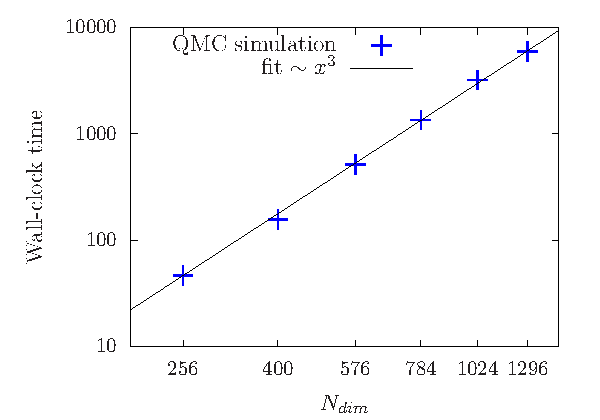
\includegraphics[scale=.8]{Figures/Size_scaling_ALF_2.pdf}
	\end{center}
	\caption{\label{fig_scaling_size}Volume scaling behavior of the auxiliary field QMC code of the ALF project on SuperMUC (phase 2/Haswell nodes) at the LRZ in Munich. The number of sites $N_{\text{dim}}$ corresponds to the system volume.
	The plot confirms that the leading scaling order is due to matrix multiplications such that the runtime is dominated by calls to ZGEMM. }
\end{figure}

For the implementation which scales linearly in $\beta$, one has to store $2\times N_{fl} \times L_{\text{Trotter}}/\texttt{NWrap}$ intermediate propagation matrices of dimension $N_{\text{dim}}\times N_{\text{dim}}$.   
Hence the memory cost scales as $ \beta N_{\text{dim}}^2$ and for  large lattices and/or low temperatures this dominates the total memory requirements that can exceed 2~GB memory for a sequential version.   

The above estimates of $\beta N_{\text{dim}}^3 $ for CPU time and $\beta N_{\text{dim}}^2 $ for memory implicitly assume Hamiltonians where the interaction  is a sum of local terms.  
Recently  Landau level projection schemes for the   regularization of continuum field theories have been introduced in the realm of the auxiliary field QMC algorithm  \cite{Ippoliti18,WangZ20}. In  this case the interaction is not local,  such that the matrices stored in  the   \texttt{Op\_V} array  of \texttt{Observable} type   are of dimension of $N_{\text{dim}}$. Since the  dimension of the  \texttt{Op\_V}   array scales as $N_{\text{dim}}$, the memory  requirement scales as $N_{\text{dim}}^3$.    In these algorithms, a single field couples to a $N_{\text{dim}} \times  N_{\text{dim}} $ matrix, such that updating  it scales as $ N_{\text{dim}}^3$.  Furthermore, and as mentioned in Sec.~\ref{sec:trotter}, for non-local  Hamiltonians the  Trotter time step has to be scaled   as $1/N_{\text{dim}}$ so as to maintain a constant systematic error.  Taking all of this into account,    yields a CPU time that scales as $\beta N_{\text{dim}}^5$.    Hence  this approach  is expensive both in memory and CPU time. 

At the heart of Monte Carlo schemes lies a random walk through the given configuration space. This is easily parallelized via MPI by associating one random walker to each MPI task. For each task, we start from a random configuration and have to invest the autocorrelation time $T_\mathrm{auto}$ to produce an equilibrated configuration.
Additionally we can also profit from an OpenMP parallelized version of the BLAS/LAPACK library for an additional speedup, which also effects equilibration overhead $N_\text{MPI}\times T_\text{auto} / N_\text{OMP}$, where $N_{\text{MPI}}$ is the number of cores and $N_{\text{OMP}}$ the number of OpenMP threads.
For a given number of independent measurements  $N_\text{meas}$, we  therefore need a wall-clock time given by
\begin{equation}\label{eqn:scaling}
T  =  \frac{T_\text{auto}}{N_\text{OMP}} \left( 1   +    \frac{N_\text{meas}}{N_\text{MPI}}  \right) \,.
\end{equation}
As we typically have $ N_\text{meas}/N_\text{MPI} \gg 1 $, 
the speedup is expected to be almost perfect, in accordance with
the performance test results for the auxiliary field
QMC code  on SuperMUC (see Fig.~\ref{fig_scaling} (left)).

For many problem sizes, 2~GB memory per MPI task (random walker) suffices such that we typically start as many MPI tasks as there are physical cores per node. Due to the large amount of CPU time spent in MKL routines, we do not profit from the hyper-threading option. For large systems, the memory requirement increases and this is tackled by increasing the amount of OpenMP threads to decrease the stress on the memory system and to simultaneously reduce the equilibration overhead (see Fig.~\ref{fig_scaling} (right)). For the displayed speedup, it was crucial to pin the MPI tasks as well as the OpenMP threads in a pattern which keeps the threads as compact as possible to profit from a shared cache. This also explains the drop in efficiency from 14 to 28 threads where the OpenMP threads are spread over both sockets. 

We store the field configurations of the random walker as checkpoints, such that a long simulation can be easily split into several short simulations. This procedure allows us to take advantage of chained jobs using the dependency chains provided by the batch system.

\begin{figure}[H]
	\begin{center}
		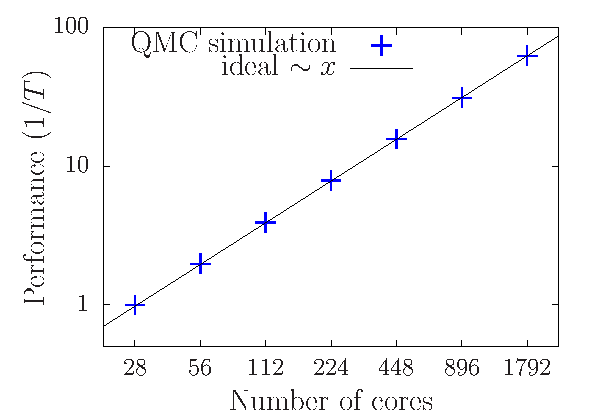
\includegraphics[scale=0.6]{Figures/MPI_scaling_ALF_2.pdf}
		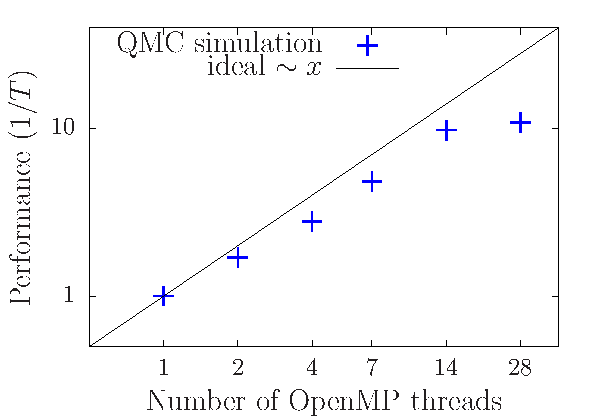
\includegraphics[scale=0.6]{Figures/OMP_scaling_ALF_2.pdf}
	\end{center}
	\caption{\label{fig_scaling} MPI (left) and OpenMP (right) scaling behavior of the auxiliary field QMC code of the ALF project on SuperMUC (phase 2/Haswell nodes) at the LRZ in Munich.
		The MPI performance data was normalized to 28 cores and was obtained using a problem size of $N_{\text{dim}}=400$. This is a medium to small system size that is the least favorable in terms of MPI synchronization effects.
		The OpenMP performance data was obtained using a problem size of $N_{\text{dim}}=1296$. Employing 2 and 4 OpenMP threads introduces some synchronization/management overhead such that the per-core performance is slightly reduced, compared to the single thread efficiency. Further increasing the amount of threads to 7 and 14 keeps the efficiency constant. The drop in performance of the 28 thread configuration is due to the architecture as the threads are now spread over both sockets of the node. To obtain the above results, it was crucial to pin the processes in a fashion that keeps the OpenMP threads as compact as possible.}
\end{figure}

%Next to the entire computational time is spent in BLAS routines such that the performance of the code will depend on the particular  implementation of this library. 
%We have found that the code performs well, and that  an efficient  OpenMP  version of the library  can be obtained merely by   loading the corresponding BLAS and LAPACK routines. 
%\mycomment{MB: Do we want to say more about OpenMP here, i.e. that it can be useful when warm-up time is a problem (and getting many CPUs is not). 
%In all other cases, the MPI parallelization is always better than the trivial OpenMP parallelization of library algos.}

\section{Conclusions and Future Directions}\label{sec:con}
% Copyright (c) 2016 The ALF project.
% This is a part of the ALF project documentation.
% The ALF project documentation by the ALF contributors is licensed
% under a Creative Commons Attribution-ShareAlike 4.0 International License.
% For the licensing details of the documentation see license.CCBYSA.
% !TEX root = doc.tex

In its present form, the  auxiliary-field QMC code of the ALF project allows us to simulate a large class of non-trivial models, both efficiently and at minimal  programming cost.  ALF 2.0 contains many advanced functionalities, including a projective formulation, various updating schemes, better control of Trotter errors, predefined structures that facilitate reuse, a large class of models, continuous fields and, finally, stochastic analytical continuation code. Also the usability of the code has improved in comparison with ALF 1.0. In particular the \href{https://git.physik.uni-wuerzburg.de/ALF/pyALF}{pyALF} project provides a Python interface to the ALF which substantially facilitates running the code for established models.

There are further capabilities that we would like to see in future versions of ALF. Introducing time-dependent Hamiltonians, for instance, will require some rethinking, but will allow, for example, to access entanglement properties of interacting fermionic systems \cite{Broecker14,Assaad14,Assaad13a,Assaad15}. Moreover, the auxiliary field approach is not the only method to simulate fermionic systems.  It would desirable to include additional lattice fermion algorithms such as the CT-INT \cite{Rubtsov05,Assaad07}. Lastly, at the more technical level, improved IO (eg. HDF5 support), post-processing, object oriented programming, as well as increased compatibility with other software projects are all certainly desirable improvements to look forward to. 

\addcontentsline{toc}{section}{Acknowledgments}
% Copyright (c) 2016 The ALF project.
% This is a part of the ALF project documentation.
% The ALF project documentation by the ALF contributors is licensed
% under a Creative Commons Attribution-ShareAlike 4.0 International License.
% For the licensing details of the documentation see license.CCBYSA.
% !TEX root = Doc.tex
%-------------------------------------------------------------------------------------
\section*{Acknowledgments} 
%-------------------------------------------------------------------------------------

We are very grateful to  S. Beyl, M. Hohenadler,  F. Parisen Toldin,  M. Raczkowski,  J. Schwab, T. Sato, Z. Wang and M. Weber,  for constant support during the development of this project.  FFA would also like to thank T.~Lang   and Z.~Y.~Meng for  developments of the auxiliary field code as well as T.~Grover. 
MB thanks the Bavarian Competence Network for Technical and Scientific High Performance Computing (KONWIHR) for financial support. FG  and JH thank the SFB-1170 for  financial support under projects Z03 and C01.  FFA thanks the DFG-funded FOR1807 and FOR1346 for partial financial support.
Part of the optimization of the code was carried out during  the  Porting and Tuning Workshop 2016 offered by the Forschungszentrum J\"ulich.
Calculations  to extensively test this package were carried out both on  SuperMUC at the  Leibniz Supercomputing Centre and on  JURECA at the J\"ulich Supercomputing Centre.
% We thank both institutions for generous allocation of computing time.
 The authors gratefully acknowledge the computing time granted by the John von Neumann Institute for Computing (NIC) and provided on the supercomputer JURECA \cite{Jureca16} at Jülich Supercomputing Centre (JSC). The authors gratefully acknowledge the Gauss Centre for Supercomputing e.V. (www.gauss-centre.eu) for funding this project by providing computing time on the GCS Supercomputer SuperMUC at Leibniz Supercomputing Centre (LRZ, www.lrz.de).
\addcontentsline{toc}{section}{References}
\bibliographystyle{./prXsty} 
\bibliography{./fassaad,./doc}
\addcontentsline{toc}{section}{License}
% Copyright (c) 2016, 2017 The ALF project.
% This is a part of the ALF project documentation.
% The ALF project documentation by the ALF contributors is licensed
% under a Creative Commons Attribution-ShareAlike 4.0 International License.
% For the licensing details of the documentation see license.CCBYSA.

% !TEX root = doc.tex

%-------------------------------------------------------------------------------------
\section{Licenses and Copyrights}
%-------------------------------------------------------------------------------------

The  ALF code  is provided as an open source software  such that it is  available  to all and we  hope that  it 
will be useful.  If you benefit from this code  we ask that you acknowledge  the ALF collaboration as described on our website \url{https://alf.physik.uni-wuerzburg.de}.  The git repository at \url{https://git.physik.uni-wuerzburg.de/ALF/ALF} gives us the tools to create a small but vibrant community around the code and provides a suitable entry point for future contributors  and future developments. 
The website is also the place where the original source files can be found.
Its public release make it necessary to add copyright headers to our source code, which is licensed under a GPL license to keep the source as well as any future work in the community. And the Creative Commons licenses are a good way to share our documentation and it is also well accepted by publishers. Therefore this document is licensed to you under a CC-BY-SA license.
This means you can share it and redistribute it as long as you cite the original source and license your changes under the same license. The details are in the file \texttt{license.CCBYSA}, which you should have received with this documentation.
To express our desire for a proper attribution we decided to make this a visible part of the license.
To that end we have exercised the rights of section 7 of GPL version 3 and have amended the license terms with an additional paragraph that expresses our wish that if an author has benefited from this code
that he/she should consider giving back a citation as specified on \url{https://alf.physik.uni-wuerzburg.de}.
This is not something that is meant to restrict your freedom of use, but something that we strongly expect to be good scientific conduct.
The original GPL license can be found in the file \texttt{license.GPL} and the additional terms can be found in \texttt{license.additional}.
In favour to our users, the ALF code contains part of the Lapack implementation version 3.6.1 from \url{http://www.netlib.org/lapack}.
Lapack is licensed under the modified BSD license whose full text can be found in \texttt{license.BSD}.\\
With that being said, we hope that the ALF code will prove to you to be a suitable and high-performance tool that enables
you to perform quantum Monte Carlo studies of solid state models of unprecedented complexity.\\
\\
The ALF project's contributors.\\
                        
%-------------------------------------------------------------------------------------
\subsection*{COPYRIGHT}
%-------------------------------------------------------------------------------------

Copyright \textcopyright ~2016-2020, The \textit{ALF} Project.\\
The ALF Project Documentation 
is licensed under a Creative Commons Attribution-ShareAlike 4.0 International License.
You are free to share and benefit from this documentation as long as this license is preserved and proper attribution to the authors is given. For details see the ALF project website \url{alf.physik.uni-wuerzburg.de} and the file \texttt{license.CCBYSA}.


\end{document}
